\documentclass[10pt,a4paper]{article}
\usepackage[utf8]{inputenc}\DeclareUnicodeCharacter{2212}{-}
\usepackage{graphicx,wrapfig,lipsum}
\usepackage[T1]{fontenc}
\usepackage{float}
\usepackage[polish]{babel}
\usepackage{wrapfig} 
\usepackage{caption}
\usepackage{subcaption}
\usepackage{mathtools}
\usepackage{lmodern}
\usepackage{enumitem}
\usepackage{lscape}
\usepackage{url}
\usepackage{longtable}
\usepackage{mhchem}
\usepackage{mathpazo}
\usepackage{booktabs}
\usepackage{pgf}
\renewcommand{\figurename}{Rys.}
\renewcommand{\tablename}{Tab.}

\author{Wojciech Noskowiak}
\title{Raport z ćwiczenia P2}
\date{Czerwiec 2021}

\usepackage{natbib}
\usepackage{graphicx}

\begin{document}

\maketitle
\tableofcontents

\begin{abstract}
    Zbadałem prędkość dryfu elektronów w zależności od natężenia przyłożonego pola elektrycznego. W celu jej uzyskania mierzyłem czas w którym elektrony przedryfowywały znany dystans w polu elektrycznym o określonym natężeniu. Przeanalizowałem uzyskane pomiary, a uzyskane wyniki przedstawiłem na wykresach do których dopasowałem odpowiednie krzywe. Podjołem też próbę obliczenia parametrów charakteryzujących dyfuzję elektronów, jednak zakończyła się ona niepowodzeniem
\end{abstract}

\newpage

\addcontentsline{toc}{section}{Wstęp}
\section*{Wstęp}
Ćwiczenia wykonałem na w oparciu o polecenia z instrukcji \cite{instrukcja}, udostępnione opracowanie \cite{opracowanie} oraz materiały wskazane na stronie pracowni \cite{dyfuzja} \cite{detektory} wykorzystując udostępniony mi układ badawczy. Celem ćwiczenia było wyznaczenie prędkości dryfu elektronów w gazie $87\%Ar + 13\% CO_2$ oraz przeanalizowanie jej zależności od przyłożonego pola elektrycznego. Badaną wartość wyliczyłem na podstawie czasu jaki elektrony potrzebowały na przelot znanego dystansu dla różnych wartości natężenia pola elektrycznego w obszarze dryfu. Dane z układu zczytywałem za pomocą oscyloskopu cyfrowego połączonego z komputerem. Odczytane z oscyloskopu dane przeanalizowałem własnym programem napisanym w języku python. Uzyskane wyniki przedstawilem na wykresach do których dopasowałem funkcje.

\section{Wprowadzenie teoretyczne}

\subsection{Motywacja \cite{instrukcja}}

We współczesnej fizyce cząstek elementarnych powszechnie wykorzystywane są detektory gazowe. Dla otrzymania informacji o przechodzących przez taki detektor cząstkach neizbędna jest znajomość prędkości dryfu w wykorzystywanym niego gazie. Układy monitorujące prędkość dryfu stanowią więc integralną część wielu detektorów. 

\subsection{Pojęcia teoretyczne}

\subsubsection{Dryf}

Dryfem nazywamy powolne przemieszczanie się cząstek naładowanych ruchem postępowym \cite{opracowanie}. Pojawienie się w gazie dryfu implikuje występowanie w nim prądu $\vec{j}$ określonego wzorem\cite{dyfuzja}:

\begin{equation*}
    \vec{j} = \sum_{k}{e_k n_k \vec{v_k}}
\end{equation*}

Gdzie indeks $k$ określa rodzaj cząstki naładowanej, a:
\begin{itemize}
    \item $e_k$ - ładunek danego  rodzaju cząstek
    \item $n_k$ - koncentracja danego rodzaju cząstek
    \item $v_k$ - prędkość dryfu cząstek danego rodzaju
\end{itemize}

Dryf cząstek może być wywołany wieloma zjawiskami, jednak w tym doświadczeniu zajmowałem się badaniem dryfu wywołanego na skutek działania zewnętrznego pola elektrycznego. Kierunek takiego dryfu jest zgodny z liniami działającego pola, a jego prędkość jest wprost proporcjonalna do natężenia tego pola\cite{opracowanie}:

\begin{equation*}
    \vec{v} = \mu \vec{E}
\end{equation*}

Gdzie $\mu$ jest współczynnikiem proporcjonalności.

\newpage

\subsubsection{Dyfuzja}

\begin{wrapfigure}{l}{6cm}
    \centering
    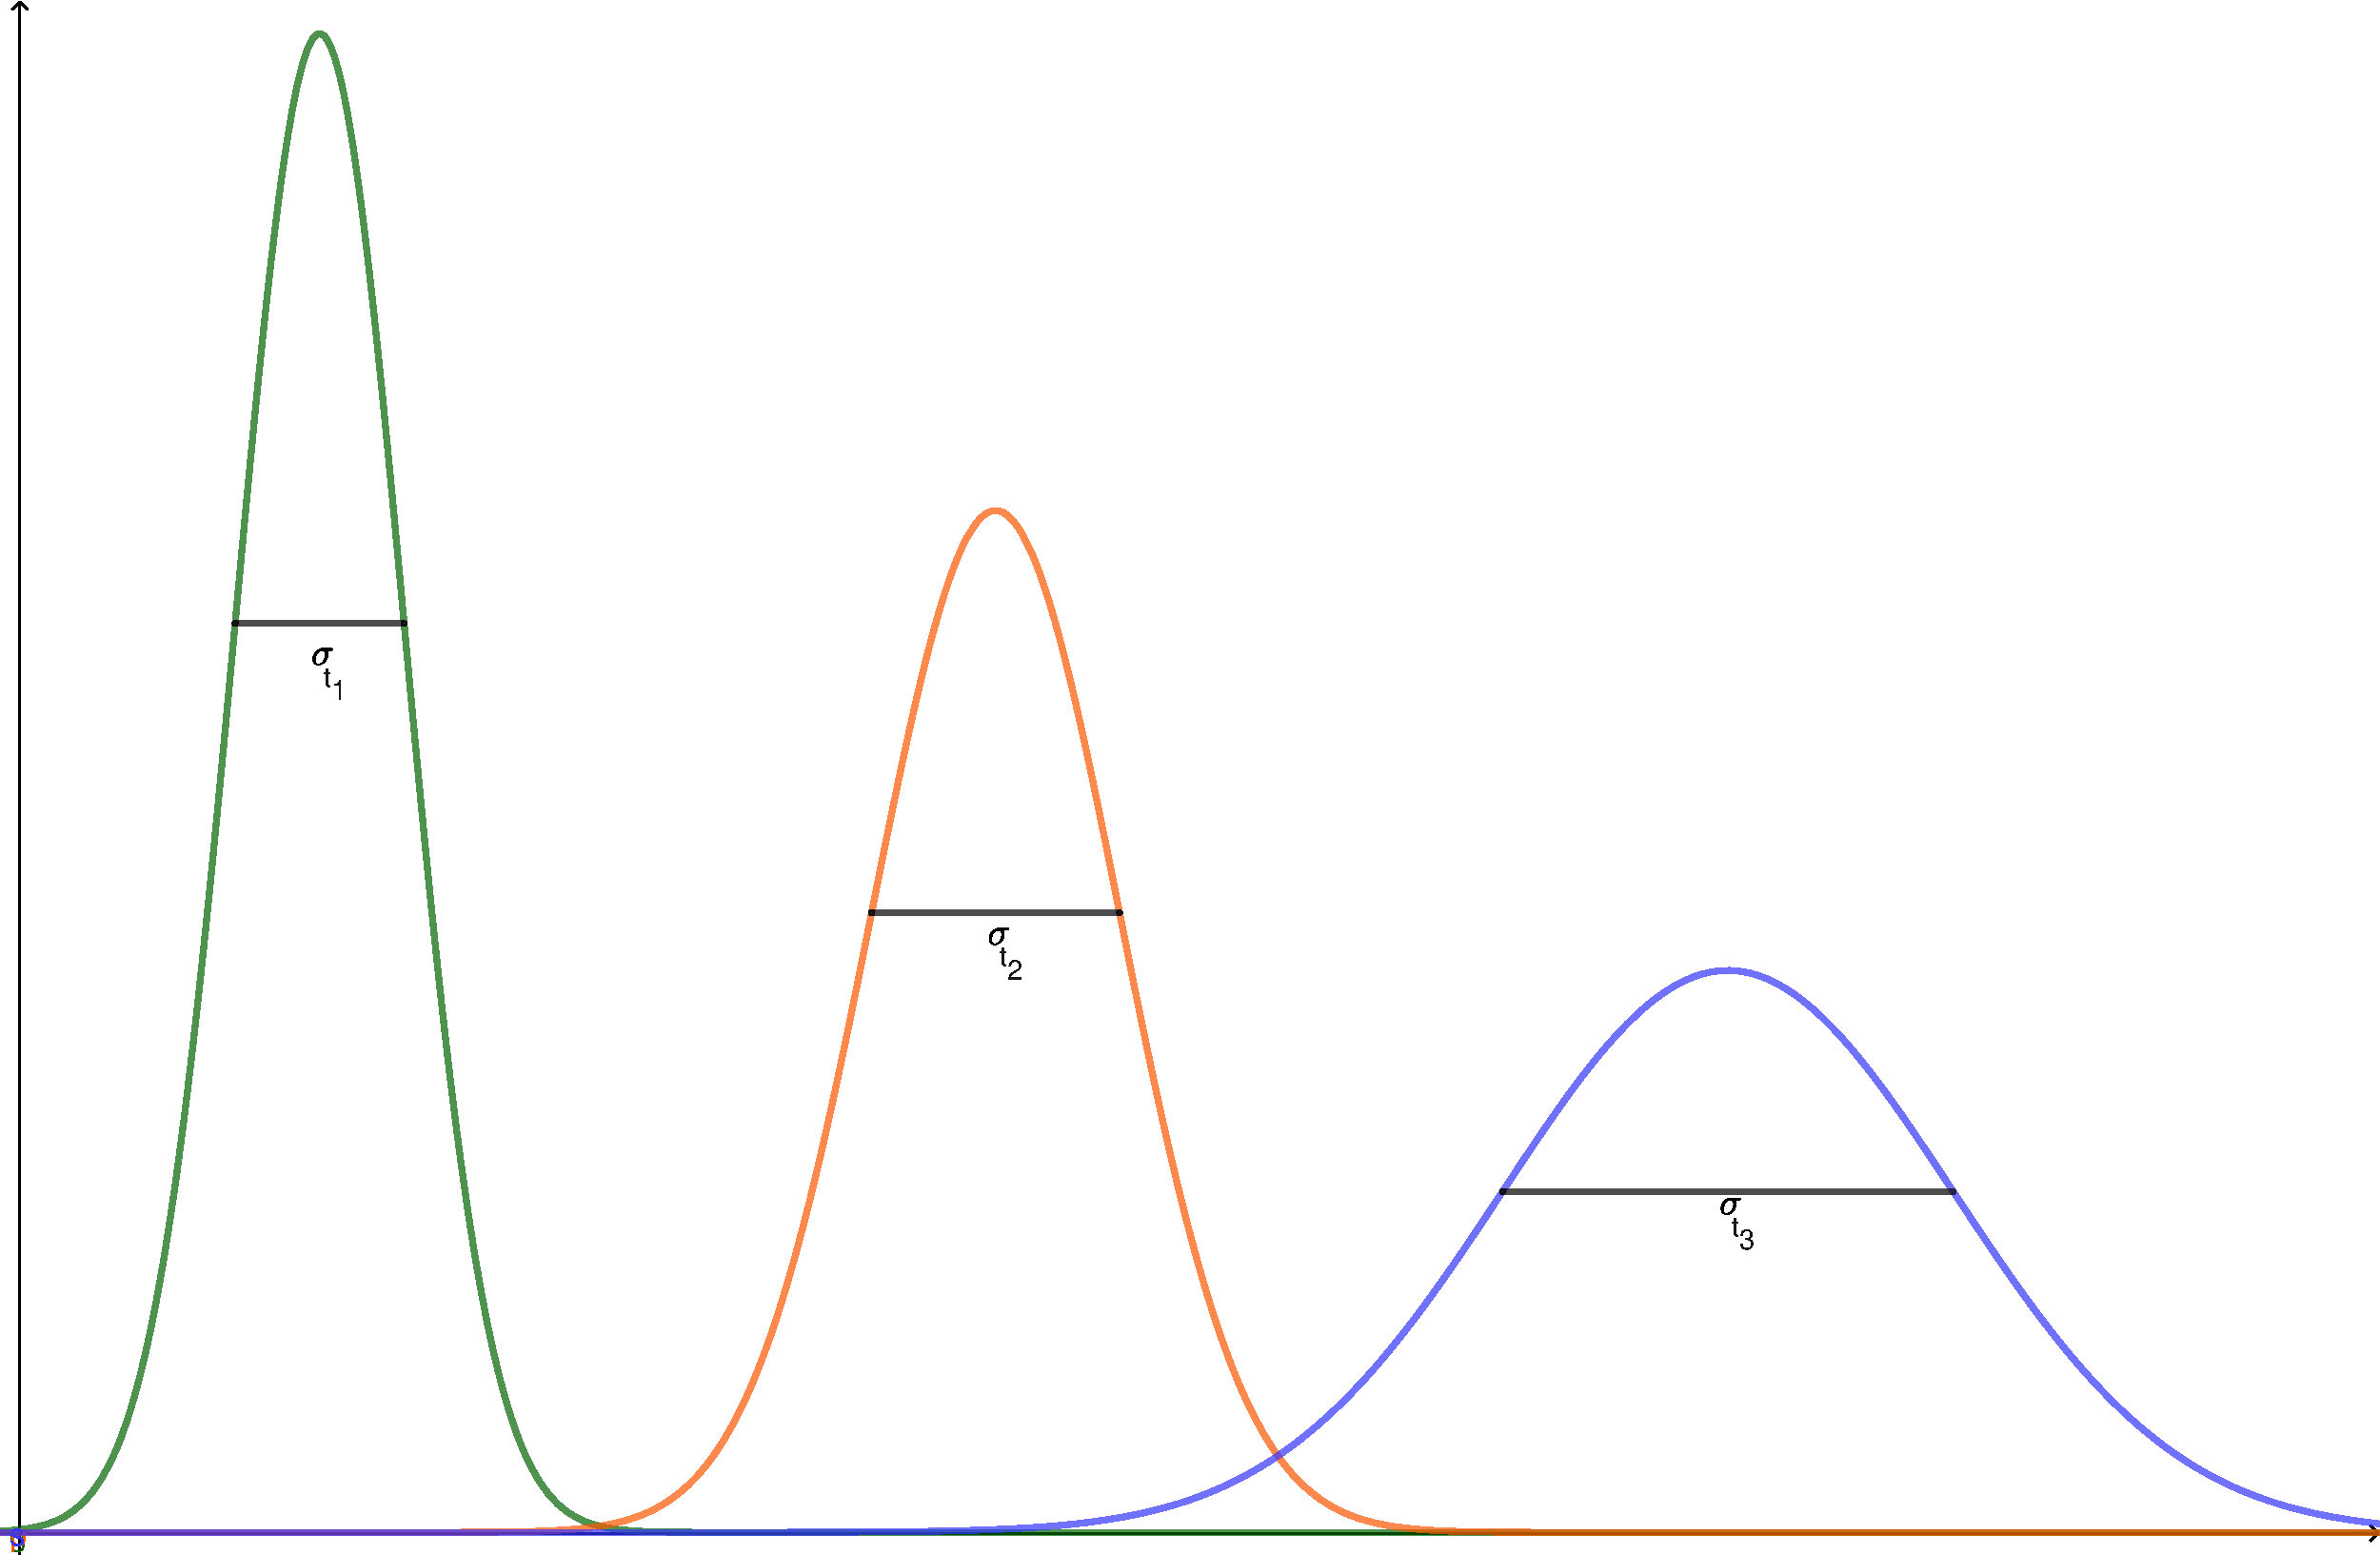
\includegraphics[width=6cm]{diagrams/dyfuzja.pdf}
    \caption{Reprezentacja rozprzestrzeniania związanego z dyfuzją. W miarę upływu czasu sygnał staje się coraz bardziej rozmyty}
    \label{dyfuzja}
\end{wrapfigure}

Dyfuzją nazywamy proces samorzutnego rozprzestrzeniania się cząstek na skutek ich nieustannych ruchów molekularno-kinetycznych. Pomimo tego że da się ją zaobserwować we wszystkich stanach skupienia substancji, najszybciej zachodzi ona w gazach. Tak więc zjawisko dyfuzji dotyczyło również badanych przeze mnie dryfujących w gazie elektronów. W przypadku dyfuzji w jednym wymiarze (wzdłuż osi poruszania się cząstek) rozmycie jest proporcjonalne do czasu dryfu cząstek.\ref{dyfuzja} Występowanie tego zjawiska wprowadza dodatkowo utrudnia wyznaczenie toru cząstki w detektorach gazowych, dla tego do uzyskania poprawnych wyników konieczna jest nie tylko znajomość prędkości dryfu elektronów w gazie wykorzystywanym przez detektor, ale i parametry charakteryzujące dyfuzję cząstek w ośrodku. Podczas badania dyfuzji określa się wartość nazywaną rozmyciem strumienia cząstek $\sigma$ \cite{dyfuzja}:

\begin{equation*}
    \sigma = \sqrt{2Dt}
\end{equation*}

Gdzie $t$ określa czas dryfu cząstek, a $D$ \cite{opracowanie}:

\begin{equation*}
    D = \frac{\vec{v}\lambda}{3}
\end{equation*}

Gdzie $\vec{v}$ określa średnią prędkość cząstek, a $\lambda$ jest stałą proporcjonalności.

\subsection{Teoria działania wykorzystywanego detektora gazowego}

\begin{wrapfigure}{r}{4cm}
    \centering
    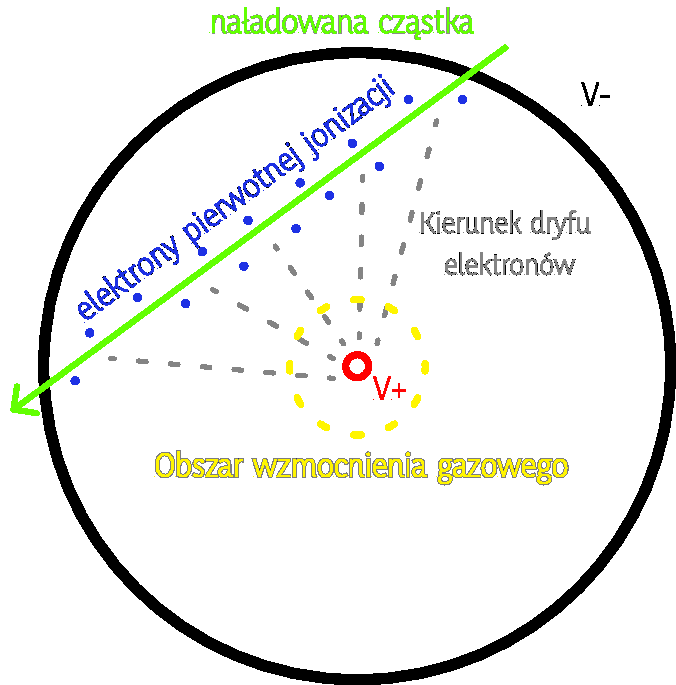
\includegraphics[width=4cm]{diagrams/detektor.pdf}
    \caption{schemat detektora gazowego}
    \label{detektor}
\end{wrapfigure}

Używany przeze mnie układ doświadczalny wykorzystywał tak zwane liczniki proporcjonalne. Są one detetorami gazowymi zbudowanymi z wypełnionego gazem cylindra oraz umieszczonego w nim koncentrycznie drutu.\ref{detektor} Podczas działania detektora wewnętrznemu drutowi zostaje nadany dodatni potencjał, a otaczającej go rurze potencjał ujemny (w przypadku mojego układu zewnętrzna rura była po prostu uziemiona). Jeśli przez działający detektor przeleci naładowana cząstak o wystarczającej energii, czyli energii większej od energii jonizacji atomów ośrodka, to spowoduje ona jonizację gazu wypełniającego detektor. Powstałe w tym procesie elektrony zaczną dryfować w kierunku naładowanego dodatnio koncentrycznego drutu. Jeśli napięcie na drucie będzie wystarczająco wysokie by w jego okolicy mogło zajść zjawisko wzmocnnienia gazowego (zjawiska w którym elektrony poruszające sie w polu elektrycznym osiągają energie wystarczające do jonizacji gazu, skutecznie zwiększając liczbę poruszających się elektronów), to po dotarciu do niego elektrony będą w stanie wytworzyć ujemny impuls elektryczny. sygnał ten może zostać odczytany oscyloskopem.\cite{detektory}

W doświadczeniu liczników proporcjonalne wykorzystywałem zarówno do detekcji cząstek $\alpha$ przelatujących przez komorę dryfową jak i do wykrywania wybitych przez nią elektronów

\section{Układ doświadczalny}

\subsection{Opis układu doświadczalnego}

\begin{figure}[h]
    \centering
    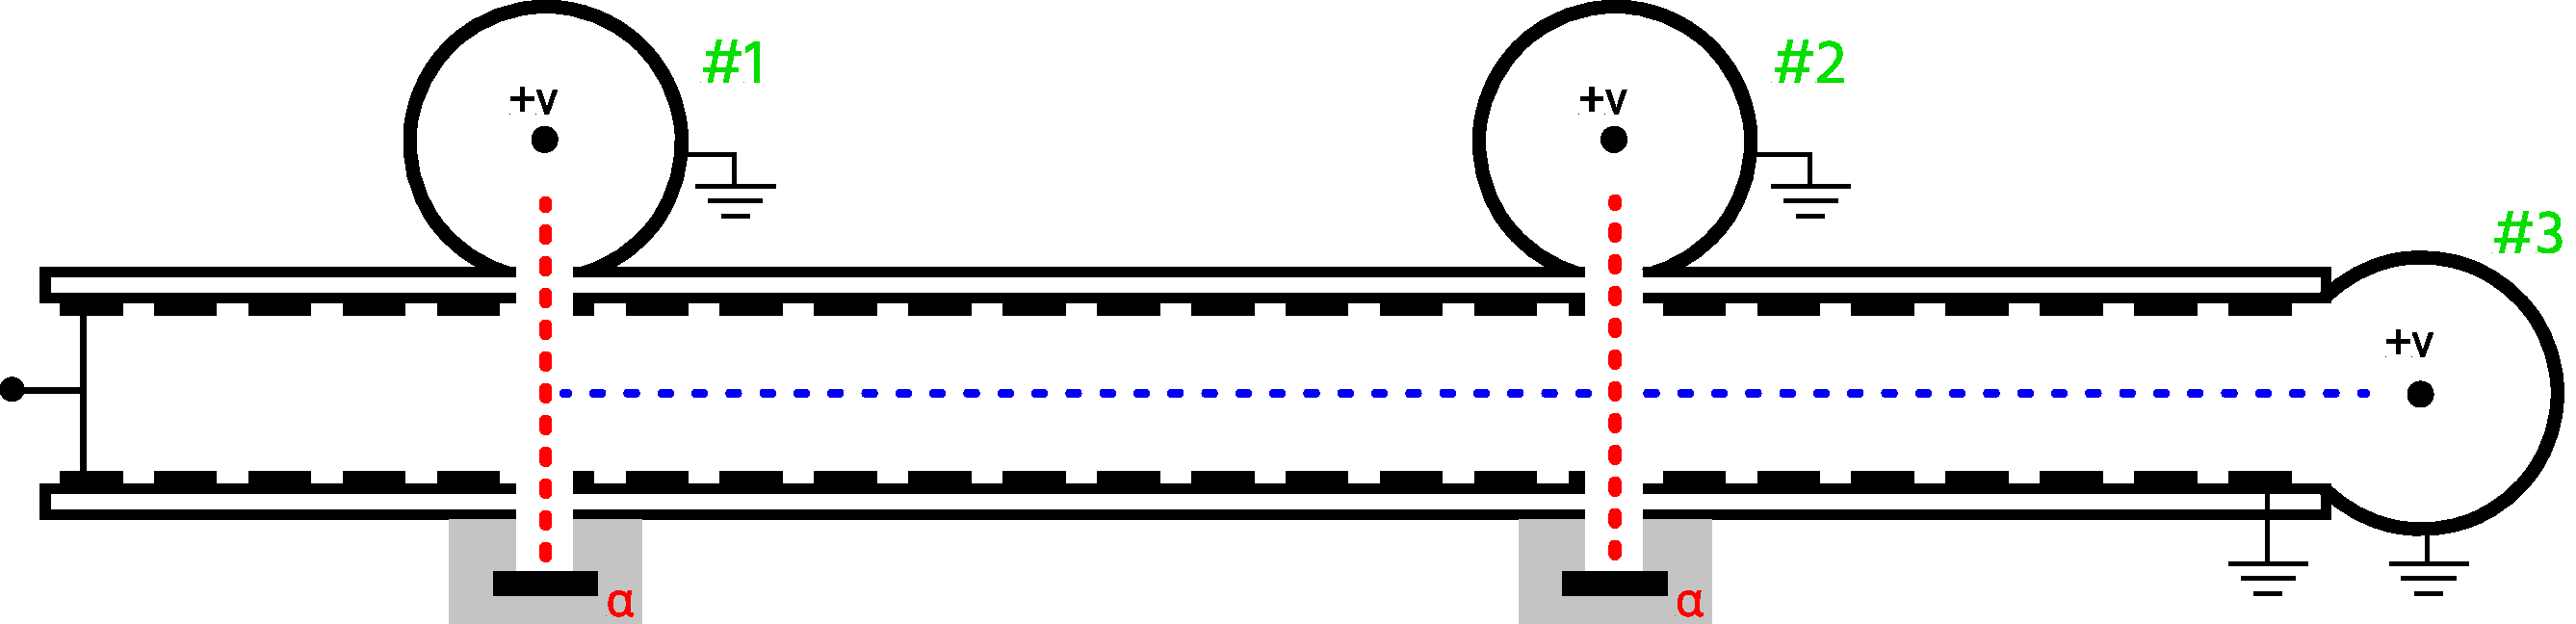
\includegraphics[width=12cm]{diagrams/uklad.pdf}
    \caption{Schemat układu badawczego }
    \label{schem}
\end{figure}

Wykorzystany przeze mnie układ doświadczalny składał się z trzech liczników propocjonalnych oraz dwóch źródeł cząstek alfa połączonych z wypełnioną gazem komorą dryfową\cite{instrukcja}. Dwa z detektorów (\#1 i \#2  na rysunku \ref{schem}) były ułożonoe po tej samej stronie komory prostopadle do dłuższego z jej boków. Po przeciwnej stronie komory na przeciw każdego z nich znajdowało się źródło cząstek alfa (na rysunku \ref{schem} zaznaczone czeroną literą $\alpha$). trzeci detektor ((na rysunku \ref{schem}) \#3) znajdował się na końcu komory dryfowej. W ściankach komory dryfowej znajdowały się metalowe paski połączone ze sobą darbinką oporową, której jeden z końców był podłączony do źródła napięcia dryfu.

\subsection{Zasada działania układu doświadczalnego}

W czasie przeprowadzania pomiarów drabinka oporowa była utrzymywana pod napięciem (napięciem dryfu). Powodowało to wystąpienie jednorodnego pola elektrycznego w komorze dryfowej. Źródła promieniowania będące częścią układu doświadczalengo ustawione były w taki sposób, że generowane przez nie cząski $\alpha$ leciały w stronę znajdującego się na przeciw niego detektora przelatując przy tym przez komorę dryfową. Pojawienie się w komorze poruszającej się cząsteczki naładowanej powodowało jonizację gazu wypełniającego komorę. W wyniku działającego na nie jednorodnego pola elektrycznego wybite elektrony zaczynały dryfowac w stronę detektora \#3. Po pewnym czasie dryfowania dociarały one do niego, powodując pojawienie się sygnału. Porównanie czasu detekcji cząstki alfa powodującej wybicie elektronu z czasem pojawienia się sygnału na \#3 pozwalało na określenie czasu dryfu elektronów pomiędzy detektorami. Jako że w komorze dryfowej na odcinku pomiędzy detektorami \#1 i \#2 występowało jednorodne pole elektryczne, a dystans pomiędzy detektorami był znany, to znajomość czasu dryfu elektronów pomiędzy tymi detektorami pozwalała wyznaczyć ich prędkość dryfu. Ten czas dało się uzyskać poprzez porównanie czas dryfu elektronów pomiędzy detektorami \#1 i \#3 z czasem dryfu między detektorami \#2 i \#3

\subsection{Budowa układu doświadczalnego}

\begin{figure}[h]
    \centering
    \includegraphics[width=9cm]{diagrams/układ.jpg}
    \caption{Zdjęcie układu badawczego \cite{opracowanie}}
    \label{zdjacie}
\end{figure}

\begin{wrapfigure}{l}{4cm}
    \centering
    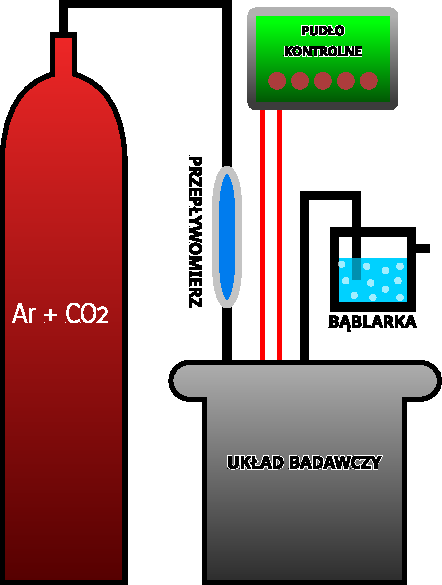
\includegraphics[width=4cm]{diagrams/schemat_budowy.pdf}
    \caption{Reprezentacja układu badawczego}
    \label{reytwitrewtrewtr}
\end{wrapfigure}
W wykorzystanym przeze mnie układzie komora dryfowa wraz z detektorami i źródłami cząstek zamontowana była w szczelnym, aluminowym cylindrze. był on połączony z oscyloskopem cyfrowym, zasilaczem oraz pudłem kontrolnym. Do cylindra doprowadzona była takrze butla zawierająca wykorzystywaną mieszaninę gazów, czyli $87\%Ar + 13\% CO_2$. W celu kompletnego wypełnienia komory dryfowej wyżej wspomniana mieszanka gazów przez godzinę przed włączeniem napięcia płyneła przez układ z szybkością 1 $Nl/h$. Przepływ gazu nie został wstrzymany na czas wykonywania pomiarów. Sygnały z drutów anodowych detektorów były wzmacniane przez liniowe wzmacniacze zasilane niskim napięciem z pudła kontrolnego. Wzmacniacze odwracały fazę, dla tego z ujemnego impulsu prądowego pojawiającego się na anodach detektorów powstawał dodatni sygnał napięciowy proporcjonalny do całkowitego ładunku lawiny elektronów Q. Wartości pola dryfu oraz napięcia na poszczególnych detektorach można było regulować przy pomocy potencjometrów znajdujących się na czołowej ścianie pudła kontrolnego. Źródłem promieniowania $\alpha$ w układzie był izotop $\ce{^{241}Am}$ generująca cząski o energii ok. $5 MeV$ \cite{instrukcja}

\begin{figure}[h]
    \centering
    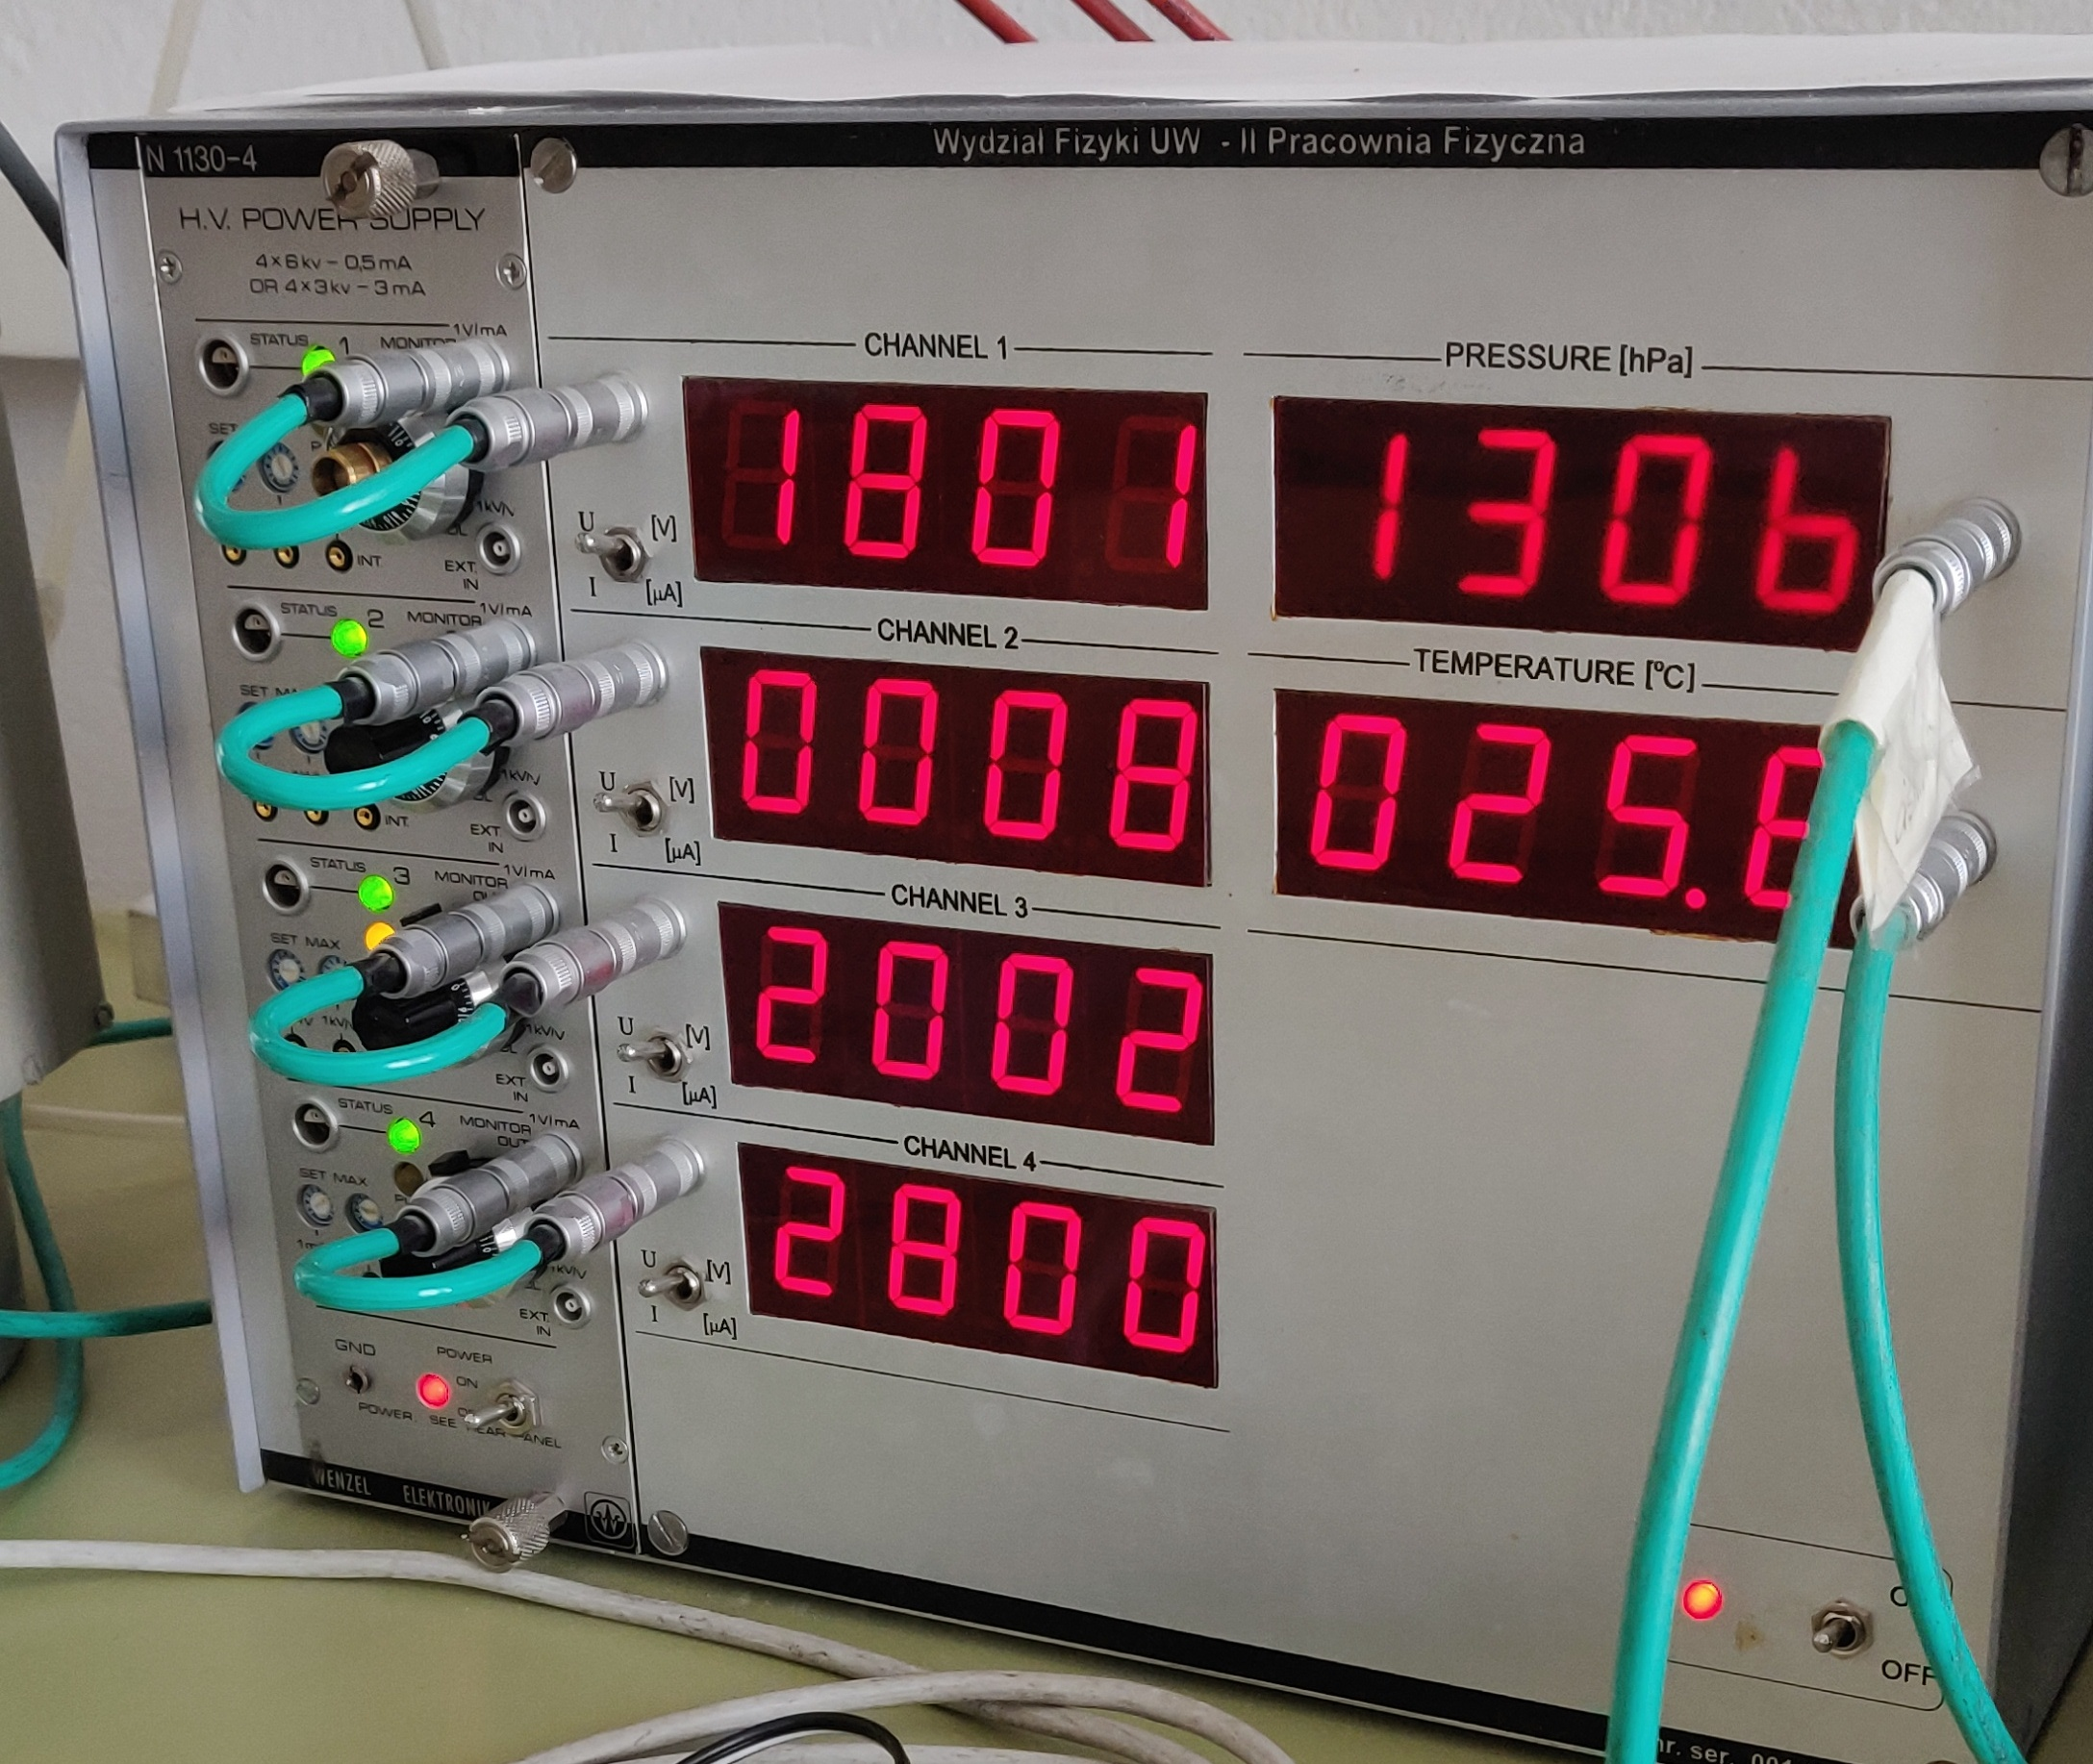
\includegraphics[width=9cm]{diagrams/IMG_20210325_145922__01.jpg}
    \caption{Zdjęcie pudła kontrolnego}
    \label{zdjacie2}
\end{figure}

\section{Opis wykonanych pomiarów}

\subsection{Metoda uzyskania pomiarów}

Pomiary rozpoczołem od włączenia układu i ustawienia napięcia na detektorach kierując się wytycznymi z instrukcji:

\begin{table}[h]
    \centering
    \caption{Napięcia na detektorach \cite{instrukcja}}
    \label{napiecia}
    \begin{tabular}{|l|l|}
        \hline
        Detektor \#1 & 1800 V \\ \hline
        Detektor \#2 & 1800 V \\ \hline
        Detektor \#3 & 2000 V \\ \hline
    \end{tabular}
\end{table}

Na wyniki pomiarów mogła mieć wpływ temperatura i ciśnienie gazu w komorze dryfowej, więc w czasie przeprowadzania pomiarów monitorowałem zachowanie tych wartości. Po odpowiednim ustawieniu napięć podłączyłem kanał A oscyloskopu z detektorem \#1, a kanał B z detektorem \#3. Potem nastaiłem napięcie dryfu na $600 V$. Oscyloskop ustawiłem w taki sposób, by po wykryciu sygnału na kanale A (czyli sygnału świadczący o wykryciu cząstki $\alpha$) zapisywał on dane z obu kanałów z pewnego krótkiego czasu z przed pojawienia się sygnału, oraz dane z pewnego okresu po pojawieniu się sygnału. Czas zbierania danych po wykryciu syganłu ustawiłem w taki sposób, by zawierał się w nim sygnał z kanału B (czyli sygnał świadczący o wykryciu elektronów wybitych przez przelatującą cząstkę). Oscyloskop automatycznie zbierał i zapisywał dane. Po wykonaniu 20 powtórzeń zapisywałem uzyskane dane, zwiększałem napięcie dryfu o $100 V$ i powtarzałem pomiary. Po uzyskaniu wyników dla napięcia dryfu $3000 V$ przełączałem kanał A oscyloskopu do detektora \#2, napięcie dryfu nastawiałem z powrotem na $600 V$ i powtarzałem proces.

\subsection{Charakterystyka uzyskanych pomiarów}

\begin{figure}[h]
    \centering
    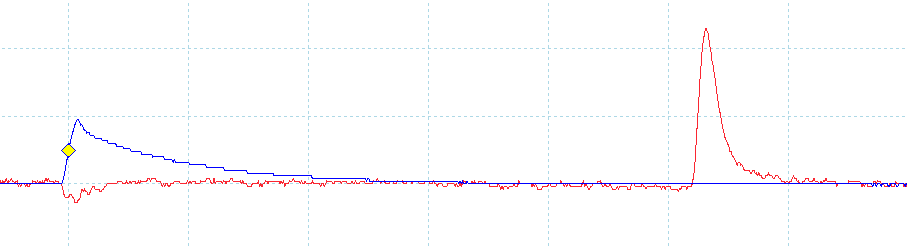
\includegraphics[width=10cm]{diagrams/13_1800_png_19.png}
    \caption{Przykładowe dane jednej serii pomiarowej}
    \label{przykladowe}
\end{figure}

Sygnały pochodzące z detektorów \#1 i \#2 różniły się znacząco do sygnałów pochodzących z detektora \#3, co jest zachowaniem zgodnym z przewidywaniami. W porównaniu do sygnałów pochodzących z detektora \#3 sygnały z detektorów \#1 i \#2 miały wyższe natężenie i wygasały wolniej\ref{przykladowe}. Sygnały ze wszystkich detektorów objawialy się zwiększeniem napięcia na kanale do którego były podpięte. jest to również zachowanie zgodne z przewidywaniami i jest wynikiem charakterystyki pracy wykorzystywanych przez układ wzmacniaczy sygnału \cite{opracowanie}

\section{Analiza uzyskanych danych}

\subsection{opis wykorzystanej metody analizy danych}

Analizowanie danych rozpoczołem od wyboru poprawnych serii pomiarowych. Sprowadzało się to do odrzucenia serii w których wartości napięcia na kanałach oscyloskopu wychodziły poza skalę.

\begin{wrapfigure}{r}{6cm}
    \centering
    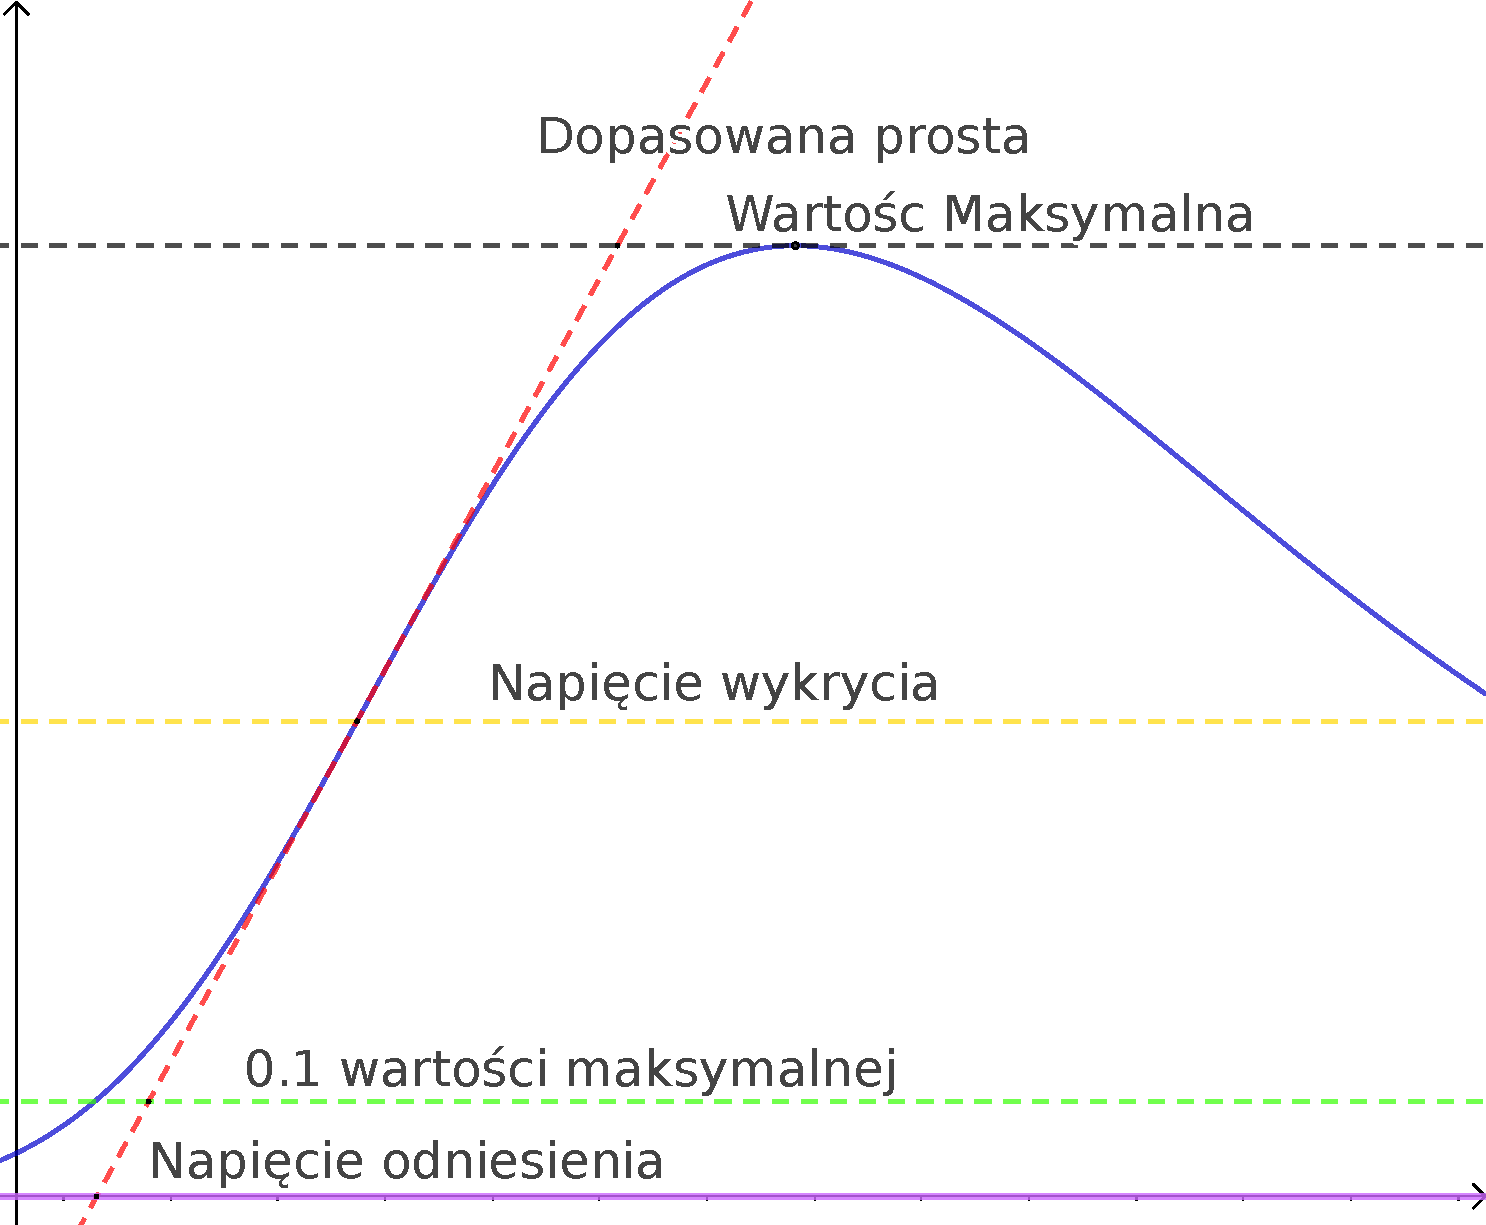
\includegraphics[width=6cm]{diagrams/analiza.pdf}
    \caption{Reprezentacja przykładowego sygnału z zaznaczonymi wartościami pomocniczymi}
    \label{pomoc}
\end{wrapfigure}

W celu uzyskania czasu dryfu elektronów na podstawie wyselekcjonowanych danych musiałem wyznaczyć moment wykrycia cząstki $\alpha$ oraz moment wykrycia elektronów, a następnie porównać ze sobą uzyskane wartości. W tym celu wyliczałem szereg wartości pomocniczych \ref{pomoc}.

Analizę danych z kanału A oscyloskopu (czyli tych świadczących o wykryciu cząstki $\alpha$) zaczynałem od wyznaczenia maksymalnego osiągniętego na kanale napięcia.
Potem analizujac dane dla pomiarów sprzed osiągnięcia maksimum ustalałem napięcie odniesienia. W celu jego wyznaczenia znajdowałem czas w którym wartosc napiecia na kanale A oscyloskopu osiągała 0.1 wartości maksymalnej, uzyskany wynik mnożyłem przez 0.75 po czym uśredniałem wartości napięcia dla czasów starszych od uzyskanej wartości. Po uzyskaniu napięcia odniesienia określałem napięcie implikuje detekcję, czyli takie które sygnał na kanale osiąga w momencie wykrycia cząstki. W tym celu uśredniałem maksymalną wartość napięcia z wyliczonym wcześniej napięciem odniesienia. Tą wartość nazywam dalej napięciem wykrycia

Następnie z pośród pomiarów dla czasów z przed osiągnięcia maksymalnego napięcia wybierałem ten o wartości najbardziej zbliżonej do napięcia wykrycia. Następnie wybierałem poprzedzające go 3 punkty oraz trzy punkty występujące po nim. Jeśli najmłodszy z wybranych w ten sposób pomiarów nie zawierał się w zbiorze punktów starszych od pomiaru maksymalnego napięcia odrzycałem go. Podobnie gdy wartość najstarszego pomiaru okazywała się być zbyt bliska wartości napięcia odniesienia to nie uwzględniałem jej w dalszych obliczeniach. Do tak wybranych punktów dopasowywałem prostą:

\begin{equation*}
    V(t) = at + b
\end{equation*}

Wyznaczone przez dopasowanie wspołczynniki podstawiałem potem do odwróconego równania prostej, które pozwalało na określenie czasu wykrycia cząstki $t_{wyk}$:

\begin{equation*}
    t_{wyk} = \frac{V_{wyk}-b}{a}
\end{equation*}

Gdzie $V_{wyk}$ wcześniej wyliczonym napięciem wykrycia

Czas wykrycia elektronów wyliczałem przeprowadzając analogiczny rachunek dla sygnału z kanału B. Analogiczny rachunek wykonywałem dla pomiarów młodszych od pomiaru dla którego występowało najwyższe napięcie na kanale w celu ustalenia czasu końca impulsu, z którego następnie wyliczałem czas trwania impulsu $t_{imp}$

\begin{equation*}
    t_{imp} = t_{wykrycia \: elektronów} - t_{konca \: impulsu}
\end{equation*}

Po przeanalizowaniu serii pomiarów wyżej opisaną metodą od uzyskanego czasu wykrycia elektronu odejmowałem czas wykrycia czastek $\alpha$. Uzyskiwałem w ten sposób czas dryfu elektronów pomiędzy detektorami dla danej serii. Tak wyliczone czasy uśredniłem dla wszystkich pomiarów wykonanych dla danego napięcia dryfu.

\begin{equation*}
    <t_{1/2-3}> = <t_{3} - t_{1/2}>
\end{equation*}

Taki rachunek przeprowadzałem dla wszystkich badanych napięć dryfu i konfiguracji podłączeń detektorów. Po uzyskaniu wyników uzyskane średnie czasy przelotu parowałem na podstawie odpowiadającego im napięcia dryfu, a następnie wyliczyłem na ich podstawie czas dryfu elektronów pomiędzy detektorami \#1 i \#2:

\begin{equation*}
    t_{12} = t_{13} - t_{23}
\end{equation*}

Na podstawie tego czasu byłem w stanie określić prędkość dryfu elektronów $v$ dla danego napięcia dryfu:

\begin{equation*}
    v = \frac{S}{t_{12}}
\end{equation*}

Gdzie $S$ jest odległoscią pomiędzy detektorem \#1 a detektorem \#2, i wynosi 4.6$[cm]$

Jako błędy pomiaru czasów przelotu przyjołem odchylenia standardowe uzyskanych wartości. Niepewność prędkości wyznaczyłem wykozystując metodę różniczki zupełnej:

\begin{equation*}
    \Delta v = \frac{S }{t^2_{12}} \Delta t + \frac{\Delta S}{t_{12}}
\end{equation*}

Wyliczone czasy dryfu jaki i związane z nimi prędkości sparowałem z odpowiadającymi im warościami zredukowanego natężenia pola dryfu, czyli warości pola drydu dla danego pomiaru podzieloną przez ciśnienie gazu w czasie wykonywania pomiaru. Uzyskane punkty przedstawiłem na wykresach

Do wyliczonych czasów przelotu $t_{12}$ dopasowałem krzywą:

\begin{equation*}
    t_{12} = t_0 + A_te^{-\frac{1}{B_t}\frac{E}{p}}
\end{equation*}

A do uzyskanych prędkości dopasowałem prostą

\begin{equation*}
    v_{12} = A_v \frac{E}{p} + B_v
\end{equation*}

Opisana powyżej metoda analizy danych nie jest perfekcyjnie dokładna, ale stanowi sposób wyznaczania dobrego przybliżenia prawdziwych czasów wykrycia

Obliczenia wykonałem programem w pythonie

\newpage

\subsection{uzyskane wyniki}

\begin{table}[h]
    \centering
    \caption{Uzyskane wyniki}
    \label{wyniki}
    \resizebox{\textwidth}{!}{%
        \begin{tabular}{|l|l|l|l|l|}
            \hline
            potencjał $\left[\frac{E}{cm*hPa}\right]$ & czas przelotu $\left[\mu s\right]$ & delta $\left[\mu s\right]$ & prędkość przelotu $\left[\frac{cm}{\mu s}\right]$ & delta $\left[\frac{cm}{\mu s}\right]$ \\ \hline
            0,459                                     & 16,13                              & 0,09                       & 0,285                                             & 0,002                                 \\ \hline
            0,536                                     & 13,74                              & 0,08                       & 0,335                                             & 0,002                                 \\ \hline
            0,613                                     & 12,01                              & 0,08                       & 0,383                                             & 0,003                                 \\ \hline
            0,689                                     & 10,68                              & 0,06                       & 0,431                                             & 0,003                                 \\ \hline
            0,766                                     & 9,55                               & 0,08                       & 0,482                                             & 0,004                                 \\ \hline
            0,842                                     & 8,63                               & 0,04                       & 0,533                                             & 0,003                                 \\ \hline
            0,919                                     & 7,89                               & 0,03                       & 0,583                                             & 0,002                                 \\ \hline
            0,995                                     & 7,27                               & 0,05                       & 0,633                                             & 0,005                                 \\ \hline
            1,072                                     & 6,68                               & 0,06                       & 0,689                                             & 0,007                                 \\ \hline
            1,149                                     & 6,25                               & 0,08                       & 0,74                                              & 0,01                                  \\ \hline
            1,225                                     & 5,77                               & 0,07                       & 0,80                                              & 0,01                                  \\ \hline
            1,302                                     & 5,43                               & 0,06                       & 0,85                                              & 0,01                                  \\ \hline
            1,378                                     & 5,08                               & 0,05                       & 0,91                                              & 0,01                                  \\ \hline
            1,455                                     & 4,82                               & 0,05                       & 0,95                                              & 0,01                                  \\ \hline
            1,531                                     & 4,57                               & 0,03                       & 1,01                                              & 0,01                                  \\ \hline
            1,608                                     & 4,33                               & 0,04                       & 1,06                                              & 0,01                                  \\ \hline
            1,685                                     & 4,10                               & 0,03                       & 1,12                                              & 0,01                                  \\ \hline
            1,761                                     & 3,91                               & 0,02                       & 1,18                                              & 0,01                                  \\ \hline
            1,838                                     & 3,70                               & 0,04                       & 1,24                                              & 0,01                                  \\ \hline
            1,914                                     & 3,55                               & 0,05                       & 1,30                                              & 0,02                                  \\ \hline
            1,991                                     & 3,38                               & 0,04                       & 1,36                                              & 0,01                                  \\ \hline
            2,067                                     & 3,23                               & 0,03                       & 1,42                                              & 0,01                                  \\ \hline
            2,144                                     & 3,03                               & 0,04                       & 1,52                                              & 0,02                                  \\ \hline
            2,221                                     & 2,95                               & 0,03                       & 1,56                                              & 0,01                                  \\ \hline
            2,297                                     & 2,86                               & 0,04                       & 1,61                                              & 0,02                                  \\ \hline
        \end{tabular}%
    }
\end{table}

\begin{figure}[h]
    \centering
    \resizebox{0.49\textwidth}{!}{%% Creator: Matplotlib, PGF backend
%%
%% To include the figure in your LaTeX document, write
%%   \input{<filename>.pgf}
%%
%% Make sure the required packages are loaded in your preamble
%%   \usepackage{pgf}
%%
%% and, on pdftex
%%   \usepackage[utf8]{inputenc}\DeclareUnicodeCharacter{2212}{-}
%%
%% or, on luatex and xetex
%%   \usepackage{unicode-math}
%%
%% Figures using additional raster images can only be included by \input if
%% they are in the same directory as the main LaTeX file. For loading figures
%% from other directories you can use the `import` package
%%   \usepackage{import}
%%
%% and then include the figures with
%%   \import{<path to file>}{<filename>.pgf}
%%
%% Matplotlib used the following preamble
%%   \usepackage{fontspec}
%%   \setmainfont{DejaVuSerif.ttf}[Path=C:/Users/wojte/Envs/yeet/Lib/site-packages/matplotlib/mpl-data/fonts/ttf/]
%%   \setsansfont{DejaVuSans.ttf}[Path=C:/Users/wojte/Envs/yeet/Lib/site-packages/matplotlib/mpl-data/fonts/ttf/]
%%   \setmonofont{DejaVuSansMono.ttf}[Path=C:/Users/wojte/Envs/yeet/Lib/site-packages/matplotlib/mpl-data/fonts/ttf/]
%%
\begingroup%
\makeatletter%
\begin{pgfpicture}%
\pgfpathrectangle{\pgfpointorigin}{\pgfqpoint{6.030000in}{8.030000in}}%
\pgfusepath{use as bounding box, clip}%
\begin{pgfscope}%
\pgfsetbuttcap%
\pgfsetmiterjoin%
\definecolor{currentfill}{rgb}{1.000000,1.000000,1.000000}%
\pgfsetfillcolor{currentfill}%
\pgfsetlinewidth{0.000000pt}%
\definecolor{currentstroke}{rgb}{1.000000,1.000000,1.000000}%
\pgfsetstrokecolor{currentstroke}%
\pgfsetdash{}{0pt}%
\pgfpathmoveto{\pgfqpoint{0.000000in}{0.000000in}}%
\pgfpathlineto{\pgfqpoint{6.030000in}{0.000000in}}%
\pgfpathlineto{\pgfqpoint{6.030000in}{8.030000in}}%
\pgfpathlineto{\pgfqpoint{0.000000in}{8.030000in}}%
\pgfpathclose%
\pgfusepath{fill}%
\end{pgfscope}%
\begin{pgfscope}%
\pgfsetbuttcap%
\pgfsetmiterjoin%
\definecolor{currentfill}{rgb}{1.000000,1.000000,1.000000}%
\pgfsetfillcolor{currentfill}%
\pgfsetlinewidth{0.000000pt}%
\definecolor{currentstroke}{rgb}{0.000000,0.000000,0.000000}%
\pgfsetstrokecolor{currentstroke}%
\pgfsetstrokeopacity{0.000000}%
\pgfsetdash{}{0pt}%
\pgfpathmoveto{\pgfqpoint{0.753750in}{1.324950in}}%
\pgfpathlineto{\pgfqpoint{5.427000in}{1.324950in}}%
\pgfpathlineto{\pgfqpoint{5.427000in}{7.066400in}}%
\pgfpathlineto{\pgfqpoint{0.753750in}{7.066400in}}%
\pgfpathclose%
\pgfusepath{fill}%
\end{pgfscope}%
\begin{pgfscope}%
\pgfsetbuttcap%
\pgfsetroundjoin%
\definecolor{currentfill}{rgb}{0.000000,0.000000,0.000000}%
\pgfsetfillcolor{currentfill}%
\pgfsetlinewidth{0.803000pt}%
\definecolor{currentstroke}{rgb}{0.000000,0.000000,0.000000}%
\pgfsetstrokecolor{currentstroke}%
\pgfsetdash{}{0pt}%
\pgfsys@defobject{currentmarker}{\pgfqpoint{0.000000in}{-0.048611in}}{\pgfqpoint{0.000000in}{0.000000in}}{%
\pgfpathmoveto{\pgfqpoint{0.000000in}{0.000000in}}%
\pgfpathlineto{\pgfqpoint{0.000000in}{-0.048611in}}%
\pgfusepath{stroke,fill}%
}%
\begin{pgfscope}%
\pgfsys@transformshift{1.109558in}{1.324950in}%
\pgfsys@useobject{currentmarker}{}%
\end{pgfscope}%
\end{pgfscope}%
\begin{pgfscope}%
\definecolor{textcolor}{rgb}{0.000000,0.000000,0.000000}%
\pgfsetstrokecolor{textcolor}%
\pgfsetfillcolor{textcolor}%
\pgftext[x=1.109558in,y=1.227728in,,top]{\color{textcolor}\sffamily\fontsize{10.000000}{12.000000}\selectfont 0.50}%
\end{pgfscope}%
\begin{pgfscope}%
\pgfsetbuttcap%
\pgfsetroundjoin%
\definecolor{currentfill}{rgb}{0.000000,0.000000,0.000000}%
\pgfsetfillcolor{currentfill}%
\pgfsetlinewidth{0.803000pt}%
\definecolor{currentstroke}{rgb}{0.000000,0.000000,0.000000}%
\pgfsetstrokecolor{currentstroke}%
\pgfsetdash{}{0pt}%
\pgfsys@defobject{currentmarker}{\pgfqpoint{0.000000in}{-0.048611in}}{\pgfqpoint{0.000000in}{0.000000in}}{%
\pgfpathmoveto{\pgfqpoint{0.000000in}{0.000000in}}%
\pgfpathlineto{\pgfqpoint{0.000000in}{-0.048611in}}%
\pgfusepath{stroke,fill}%
}%
\begin{pgfscope}%
\pgfsys@transformshift{1.673606in}{1.324950in}%
\pgfsys@useobject{currentmarker}{}%
\end{pgfscope}%
\end{pgfscope}%
\begin{pgfscope}%
\definecolor{textcolor}{rgb}{0.000000,0.000000,0.000000}%
\pgfsetstrokecolor{textcolor}%
\pgfsetfillcolor{textcolor}%
\pgftext[x=1.673606in,y=1.227728in,,top]{\color{textcolor}\sffamily\fontsize{10.000000}{12.000000}\selectfont 0.75}%
\end{pgfscope}%
\begin{pgfscope}%
\pgfsetbuttcap%
\pgfsetroundjoin%
\definecolor{currentfill}{rgb}{0.000000,0.000000,0.000000}%
\pgfsetfillcolor{currentfill}%
\pgfsetlinewidth{0.803000pt}%
\definecolor{currentstroke}{rgb}{0.000000,0.000000,0.000000}%
\pgfsetstrokecolor{currentstroke}%
\pgfsetdash{}{0pt}%
\pgfsys@defobject{currentmarker}{\pgfqpoint{0.000000in}{-0.048611in}}{\pgfqpoint{0.000000in}{0.000000in}}{%
\pgfpathmoveto{\pgfqpoint{0.000000in}{0.000000in}}%
\pgfpathlineto{\pgfqpoint{0.000000in}{-0.048611in}}%
\pgfusepath{stroke,fill}%
}%
\begin{pgfscope}%
\pgfsys@transformshift{2.237654in}{1.324950in}%
\pgfsys@useobject{currentmarker}{}%
\end{pgfscope}%
\end{pgfscope}%
\begin{pgfscope}%
\definecolor{textcolor}{rgb}{0.000000,0.000000,0.000000}%
\pgfsetstrokecolor{textcolor}%
\pgfsetfillcolor{textcolor}%
\pgftext[x=2.237654in,y=1.227728in,,top]{\color{textcolor}\sffamily\fontsize{10.000000}{12.000000}\selectfont 1.00}%
\end{pgfscope}%
\begin{pgfscope}%
\pgfsetbuttcap%
\pgfsetroundjoin%
\definecolor{currentfill}{rgb}{0.000000,0.000000,0.000000}%
\pgfsetfillcolor{currentfill}%
\pgfsetlinewidth{0.803000pt}%
\definecolor{currentstroke}{rgb}{0.000000,0.000000,0.000000}%
\pgfsetstrokecolor{currentstroke}%
\pgfsetdash{}{0pt}%
\pgfsys@defobject{currentmarker}{\pgfqpoint{0.000000in}{-0.048611in}}{\pgfqpoint{0.000000in}{0.000000in}}{%
\pgfpathmoveto{\pgfqpoint{0.000000in}{0.000000in}}%
\pgfpathlineto{\pgfqpoint{0.000000in}{-0.048611in}}%
\pgfusepath{stroke,fill}%
}%
\begin{pgfscope}%
\pgfsys@transformshift{2.801702in}{1.324950in}%
\pgfsys@useobject{currentmarker}{}%
\end{pgfscope}%
\end{pgfscope}%
\begin{pgfscope}%
\definecolor{textcolor}{rgb}{0.000000,0.000000,0.000000}%
\pgfsetstrokecolor{textcolor}%
\pgfsetfillcolor{textcolor}%
\pgftext[x=2.801702in,y=1.227728in,,top]{\color{textcolor}\sffamily\fontsize{10.000000}{12.000000}\selectfont 1.25}%
\end{pgfscope}%
\begin{pgfscope}%
\pgfsetbuttcap%
\pgfsetroundjoin%
\definecolor{currentfill}{rgb}{0.000000,0.000000,0.000000}%
\pgfsetfillcolor{currentfill}%
\pgfsetlinewidth{0.803000pt}%
\definecolor{currentstroke}{rgb}{0.000000,0.000000,0.000000}%
\pgfsetstrokecolor{currentstroke}%
\pgfsetdash{}{0pt}%
\pgfsys@defobject{currentmarker}{\pgfqpoint{0.000000in}{-0.048611in}}{\pgfqpoint{0.000000in}{0.000000in}}{%
\pgfpathmoveto{\pgfqpoint{0.000000in}{0.000000in}}%
\pgfpathlineto{\pgfqpoint{0.000000in}{-0.048611in}}%
\pgfusepath{stroke,fill}%
}%
\begin{pgfscope}%
\pgfsys@transformshift{3.365750in}{1.324950in}%
\pgfsys@useobject{currentmarker}{}%
\end{pgfscope}%
\end{pgfscope}%
\begin{pgfscope}%
\definecolor{textcolor}{rgb}{0.000000,0.000000,0.000000}%
\pgfsetstrokecolor{textcolor}%
\pgfsetfillcolor{textcolor}%
\pgftext[x=3.365750in,y=1.227728in,,top]{\color{textcolor}\sffamily\fontsize{10.000000}{12.000000}\selectfont 1.50}%
\end{pgfscope}%
\begin{pgfscope}%
\pgfsetbuttcap%
\pgfsetroundjoin%
\definecolor{currentfill}{rgb}{0.000000,0.000000,0.000000}%
\pgfsetfillcolor{currentfill}%
\pgfsetlinewidth{0.803000pt}%
\definecolor{currentstroke}{rgb}{0.000000,0.000000,0.000000}%
\pgfsetstrokecolor{currentstroke}%
\pgfsetdash{}{0pt}%
\pgfsys@defobject{currentmarker}{\pgfqpoint{0.000000in}{-0.048611in}}{\pgfqpoint{0.000000in}{0.000000in}}{%
\pgfpathmoveto{\pgfqpoint{0.000000in}{0.000000in}}%
\pgfpathlineto{\pgfqpoint{0.000000in}{-0.048611in}}%
\pgfusepath{stroke,fill}%
}%
\begin{pgfscope}%
\pgfsys@transformshift{3.929798in}{1.324950in}%
\pgfsys@useobject{currentmarker}{}%
\end{pgfscope}%
\end{pgfscope}%
\begin{pgfscope}%
\definecolor{textcolor}{rgb}{0.000000,0.000000,0.000000}%
\pgfsetstrokecolor{textcolor}%
\pgfsetfillcolor{textcolor}%
\pgftext[x=3.929798in,y=1.227728in,,top]{\color{textcolor}\sffamily\fontsize{10.000000}{12.000000}\selectfont 1.75}%
\end{pgfscope}%
\begin{pgfscope}%
\pgfsetbuttcap%
\pgfsetroundjoin%
\definecolor{currentfill}{rgb}{0.000000,0.000000,0.000000}%
\pgfsetfillcolor{currentfill}%
\pgfsetlinewidth{0.803000pt}%
\definecolor{currentstroke}{rgb}{0.000000,0.000000,0.000000}%
\pgfsetstrokecolor{currentstroke}%
\pgfsetdash{}{0pt}%
\pgfsys@defobject{currentmarker}{\pgfqpoint{0.000000in}{-0.048611in}}{\pgfqpoint{0.000000in}{0.000000in}}{%
\pgfpathmoveto{\pgfqpoint{0.000000in}{0.000000in}}%
\pgfpathlineto{\pgfqpoint{0.000000in}{-0.048611in}}%
\pgfusepath{stroke,fill}%
}%
\begin{pgfscope}%
\pgfsys@transformshift{4.493845in}{1.324950in}%
\pgfsys@useobject{currentmarker}{}%
\end{pgfscope}%
\end{pgfscope}%
\begin{pgfscope}%
\definecolor{textcolor}{rgb}{0.000000,0.000000,0.000000}%
\pgfsetstrokecolor{textcolor}%
\pgfsetfillcolor{textcolor}%
\pgftext[x=4.493845in,y=1.227728in,,top]{\color{textcolor}\sffamily\fontsize{10.000000}{12.000000}\selectfont 2.00}%
\end{pgfscope}%
\begin{pgfscope}%
\pgfsetbuttcap%
\pgfsetroundjoin%
\definecolor{currentfill}{rgb}{0.000000,0.000000,0.000000}%
\pgfsetfillcolor{currentfill}%
\pgfsetlinewidth{0.803000pt}%
\definecolor{currentstroke}{rgb}{0.000000,0.000000,0.000000}%
\pgfsetstrokecolor{currentstroke}%
\pgfsetdash{}{0pt}%
\pgfsys@defobject{currentmarker}{\pgfqpoint{0.000000in}{-0.048611in}}{\pgfqpoint{0.000000in}{0.000000in}}{%
\pgfpathmoveto{\pgfqpoint{0.000000in}{0.000000in}}%
\pgfpathlineto{\pgfqpoint{0.000000in}{-0.048611in}}%
\pgfusepath{stroke,fill}%
}%
\begin{pgfscope}%
\pgfsys@transformshift{5.057893in}{1.324950in}%
\pgfsys@useobject{currentmarker}{}%
\end{pgfscope}%
\end{pgfscope}%
\begin{pgfscope}%
\definecolor{textcolor}{rgb}{0.000000,0.000000,0.000000}%
\pgfsetstrokecolor{textcolor}%
\pgfsetfillcolor{textcolor}%
\pgftext[x=5.057893in,y=1.227728in,,top]{\color{textcolor}\sffamily\fontsize{10.000000}{12.000000}\selectfont 2.25}%
\end{pgfscope}%
\begin{pgfscope}%
\definecolor{textcolor}{rgb}{0.000000,0.000000,0.000000}%
\pgfsetstrokecolor{textcolor}%
\pgfsetfillcolor{textcolor}%
\pgftext[x=3.090375in,y=1.037759in,,top]{\color{textcolor}\sffamily\fontsize{20.000000}{12.000000}\selectfont $\frac{E}{p} \left[\frac{V}{cm*hPa}\right]$}%
\end{pgfscope}%
\begin{pgfscope}%
\pgfsetbuttcap%
\pgfsetroundjoin%
\definecolor{currentfill}{rgb}{0.000000,0.000000,0.000000}%
\pgfsetfillcolor{currentfill}%
\pgfsetlinewidth{0.803000pt}%
\definecolor{currentstroke}{rgb}{0.000000,0.000000,0.000000}%
\pgfsetstrokecolor{currentstroke}%
\pgfsetdash{}{0pt}%
\pgfsys@defobject{currentmarker}{\pgfqpoint{-0.048611in}{0.000000in}}{\pgfqpoint{-0.000000in}{0.000000in}}{%
\pgfpathmoveto{\pgfqpoint{-0.000000in}{0.000000in}}%
\pgfpathlineto{\pgfqpoint{-0.048611in}{0.000000in}}%
\pgfusepath{stroke,fill}%
}%
\begin{pgfscope}%
\pgfsys@transformshift{0.753750in}{1.380157in}%
\pgfsys@useobject{currentmarker}{}%
\end{pgfscope}%
\end{pgfscope}%
\begin{pgfscope}%
\definecolor{textcolor}{rgb}{0.000000,0.000000,0.000000}%
\pgfsetstrokecolor{textcolor}%
\pgfsetfillcolor{textcolor}%
\pgftext[x=0.435648in, y=1.327395in, left, base]{\color{textcolor}\sffamily\fontsize{10.000000}{12.000000}\selectfont 0.2}%
\end{pgfscope}%
\begin{pgfscope}%
\pgfsetbuttcap%
\pgfsetroundjoin%
\definecolor{currentfill}{rgb}{0.000000,0.000000,0.000000}%
\pgfsetfillcolor{currentfill}%
\pgfsetlinewidth{0.803000pt}%
\definecolor{currentstroke}{rgb}{0.000000,0.000000,0.000000}%
\pgfsetstrokecolor{currentstroke}%
\pgfsetdash{}{0pt}%
\pgfsys@defobject{currentmarker}{\pgfqpoint{-0.048611in}{0.000000in}}{\pgfqpoint{-0.000000in}{0.000000in}}{%
\pgfpathmoveto{\pgfqpoint{-0.000000in}{0.000000in}}%
\pgfpathlineto{\pgfqpoint{-0.048611in}{0.000000in}}%
\pgfusepath{stroke,fill}%
}%
\begin{pgfscope}%
\pgfsys@transformshift{0.753750in}{2.138428in}%
\pgfsys@useobject{currentmarker}{}%
\end{pgfscope}%
\end{pgfscope}%
\begin{pgfscope}%
\definecolor{textcolor}{rgb}{0.000000,0.000000,0.000000}%
\pgfsetstrokecolor{textcolor}%
\pgfsetfillcolor{textcolor}%
\pgftext[x=0.435648in, y=2.085667in, left, base]{\color{textcolor}\sffamily\fontsize{10.000000}{12.000000}\selectfont 0.4}%
\end{pgfscope}%
\begin{pgfscope}%
\pgfsetbuttcap%
\pgfsetroundjoin%
\definecolor{currentfill}{rgb}{0.000000,0.000000,0.000000}%
\pgfsetfillcolor{currentfill}%
\pgfsetlinewidth{0.803000pt}%
\definecolor{currentstroke}{rgb}{0.000000,0.000000,0.000000}%
\pgfsetstrokecolor{currentstroke}%
\pgfsetdash{}{0pt}%
\pgfsys@defobject{currentmarker}{\pgfqpoint{-0.048611in}{0.000000in}}{\pgfqpoint{-0.000000in}{0.000000in}}{%
\pgfpathmoveto{\pgfqpoint{-0.000000in}{0.000000in}}%
\pgfpathlineto{\pgfqpoint{-0.048611in}{0.000000in}}%
\pgfusepath{stroke,fill}%
}%
\begin{pgfscope}%
\pgfsys@transformshift{0.753750in}{2.896700in}%
\pgfsys@useobject{currentmarker}{}%
\end{pgfscope}%
\end{pgfscope}%
\begin{pgfscope}%
\definecolor{textcolor}{rgb}{0.000000,0.000000,0.000000}%
\pgfsetstrokecolor{textcolor}%
\pgfsetfillcolor{textcolor}%
\pgftext[x=0.435648in, y=2.843939in, left, base]{\color{textcolor}\sffamily\fontsize{10.000000}{12.000000}\selectfont 0.6}%
\end{pgfscope}%
\begin{pgfscope}%
\pgfsetbuttcap%
\pgfsetroundjoin%
\definecolor{currentfill}{rgb}{0.000000,0.000000,0.000000}%
\pgfsetfillcolor{currentfill}%
\pgfsetlinewidth{0.803000pt}%
\definecolor{currentstroke}{rgb}{0.000000,0.000000,0.000000}%
\pgfsetstrokecolor{currentstroke}%
\pgfsetdash{}{0pt}%
\pgfsys@defobject{currentmarker}{\pgfqpoint{-0.048611in}{0.000000in}}{\pgfqpoint{-0.000000in}{0.000000in}}{%
\pgfpathmoveto{\pgfqpoint{-0.000000in}{0.000000in}}%
\pgfpathlineto{\pgfqpoint{-0.048611in}{0.000000in}}%
\pgfusepath{stroke,fill}%
}%
\begin{pgfscope}%
\pgfsys@transformshift{0.753750in}{3.654972in}%
\pgfsys@useobject{currentmarker}{}%
\end{pgfscope}%
\end{pgfscope}%
\begin{pgfscope}%
\definecolor{textcolor}{rgb}{0.000000,0.000000,0.000000}%
\pgfsetstrokecolor{textcolor}%
\pgfsetfillcolor{textcolor}%
\pgftext[x=0.435648in, y=3.602210in, left, base]{\color{textcolor}\sffamily\fontsize{10.000000}{12.000000}\selectfont 0.8}%
\end{pgfscope}%
\begin{pgfscope}%
\pgfsetbuttcap%
\pgfsetroundjoin%
\definecolor{currentfill}{rgb}{0.000000,0.000000,0.000000}%
\pgfsetfillcolor{currentfill}%
\pgfsetlinewidth{0.803000pt}%
\definecolor{currentstroke}{rgb}{0.000000,0.000000,0.000000}%
\pgfsetstrokecolor{currentstroke}%
\pgfsetdash{}{0pt}%
\pgfsys@defobject{currentmarker}{\pgfqpoint{-0.048611in}{0.000000in}}{\pgfqpoint{-0.000000in}{0.000000in}}{%
\pgfpathmoveto{\pgfqpoint{-0.000000in}{0.000000in}}%
\pgfpathlineto{\pgfqpoint{-0.048611in}{0.000000in}}%
\pgfusepath{stroke,fill}%
}%
\begin{pgfscope}%
\pgfsys@transformshift{0.753750in}{4.413243in}%
\pgfsys@useobject{currentmarker}{}%
\end{pgfscope}%
\end{pgfscope}%
\begin{pgfscope}%
\definecolor{textcolor}{rgb}{0.000000,0.000000,0.000000}%
\pgfsetstrokecolor{textcolor}%
\pgfsetfillcolor{textcolor}%
\pgftext[x=0.435648in, y=4.360482in, left, base]{\color{textcolor}\sffamily\fontsize{10.000000}{12.000000}\selectfont 1.0}%
\end{pgfscope}%
\begin{pgfscope}%
\pgfsetbuttcap%
\pgfsetroundjoin%
\definecolor{currentfill}{rgb}{0.000000,0.000000,0.000000}%
\pgfsetfillcolor{currentfill}%
\pgfsetlinewidth{0.803000pt}%
\definecolor{currentstroke}{rgb}{0.000000,0.000000,0.000000}%
\pgfsetstrokecolor{currentstroke}%
\pgfsetdash{}{0pt}%
\pgfsys@defobject{currentmarker}{\pgfqpoint{-0.048611in}{0.000000in}}{\pgfqpoint{-0.000000in}{0.000000in}}{%
\pgfpathmoveto{\pgfqpoint{-0.000000in}{0.000000in}}%
\pgfpathlineto{\pgfqpoint{-0.048611in}{0.000000in}}%
\pgfusepath{stroke,fill}%
}%
\begin{pgfscope}%
\pgfsys@transformshift{0.753750in}{5.171515in}%
\pgfsys@useobject{currentmarker}{}%
\end{pgfscope}%
\end{pgfscope}%
\begin{pgfscope}%
\definecolor{textcolor}{rgb}{0.000000,0.000000,0.000000}%
\pgfsetstrokecolor{textcolor}%
\pgfsetfillcolor{textcolor}%
\pgftext[x=0.435648in, y=5.118753in, left, base]{\color{textcolor}\sffamily\fontsize{10.000000}{12.000000}\selectfont 1.2}%
\end{pgfscope}%
\begin{pgfscope}%
\pgfsetbuttcap%
\pgfsetroundjoin%
\definecolor{currentfill}{rgb}{0.000000,0.000000,0.000000}%
\pgfsetfillcolor{currentfill}%
\pgfsetlinewidth{0.803000pt}%
\definecolor{currentstroke}{rgb}{0.000000,0.000000,0.000000}%
\pgfsetstrokecolor{currentstroke}%
\pgfsetdash{}{0pt}%
\pgfsys@defobject{currentmarker}{\pgfqpoint{-0.048611in}{0.000000in}}{\pgfqpoint{-0.000000in}{0.000000in}}{%
\pgfpathmoveto{\pgfqpoint{-0.000000in}{0.000000in}}%
\pgfpathlineto{\pgfqpoint{-0.048611in}{0.000000in}}%
\pgfusepath{stroke,fill}%
}%
\begin{pgfscope}%
\pgfsys@transformshift{0.753750in}{5.929787in}%
\pgfsys@useobject{currentmarker}{}%
\end{pgfscope}%
\end{pgfscope}%
\begin{pgfscope}%
\definecolor{textcolor}{rgb}{0.000000,0.000000,0.000000}%
\pgfsetstrokecolor{textcolor}%
\pgfsetfillcolor{textcolor}%
\pgftext[x=0.435648in, y=5.877025in, left, base]{\color{textcolor}\sffamily\fontsize{10.000000}{12.000000}\selectfont 1.4}%
\end{pgfscope}%
\begin{pgfscope}%
\pgfsetbuttcap%
\pgfsetroundjoin%
\definecolor{currentfill}{rgb}{0.000000,0.000000,0.000000}%
\pgfsetfillcolor{currentfill}%
\pgfsetlinewidth{0.803000pt}%
\definecolor{currentstroke}{rgb}{0.000000,0.000000,0.000000}%
\pgfsetstrokecolor{currentstroke}%
\pgfsetdash{}{0pt}%
\pgfsys@defobject{currentmarker}{\pgfqpoint{-0.048611in}{0.000000in}}{\pgfqpoint{-0.000000in}{0.000000in}}{%
\pgfpathmoveto{\pgfqpoint{-0.000000in}{0.000000in}}%
\pgfpathlineto{\pgfqpoint{-0.048611in}{0.000000in}}%
\pgfusepath{stroke,fill}%
}%
\begin{pgfscope}%
\pgfsys@transformshift{0.753750in}{6.688058in}%
\pgfsys@useobject{currentmarker}{}%
\end{pgfscope}%
\end{pgfscope}%
\begin{pgfscope}%
\definecolor{textcolor}{rgb}{0.000000,0.000000,0.000000}%
\pgfsetstrokecolor{textcolor}%
\pgfsetfillcolor{textcolor}%
\pgftext[x=0.435648in, y=6.635297in, left, base]{\color{textcolor}\sffamily\fontsize{10.000000}{12.000000}\selectfont 1.6}%
\end{pgfscope}%
\begin{pgfscope}%
\definecolor{textcolor}{rgb}{0.000000,0.000000,0.000000}%
\pgfsetstrokecolor{textcolor}%
\pgfsetfillcolor{textcolor}%
\pgftext[x=0.380093in,y=4.195675in,,bottom,rotate=90.000000]{\color{textcolor}\sffamily\fontsize{20.000000}{12.000000}\selectfont $v_{12} \left[\frac{cm}{\mu s}\right]$}%
\end{pgfscope}%
\begin{pgfscope}%
\pgfpathrectangle{\pgfqpoint{0.753750in}{1.324950in}}{\pgfqpoint{4.673250in}{5.741450in}}%
\pgfusepath{clip}%
\pgfsetbuttcap%
\pgfsetroundjoin%
\pgfsetlinewidth{1.505625pt}%
\definecolor{currentstroke}{rgb}{0.000000,0.000000,0.000000}%
\pgfsetstrokecolor{currentstroke}%
\pgfsetdash{}{0pt}%
\pgfpathmoveto{\pgfqpoint{1.017997in}{1.697499in}}%
\pgfpathlineto{\pgfqpoint{1.017997in}{1.709000in}}%
\pgfusepath{stroke}%
\end{pgfscope}%
\begin{pgfscope}%
\pgfpathrectangle{\pgfqpoint{0.753750in}{1.324950in}}{\pgfqpoint{4.673250in}{5.741450in}}%
\pgfusepath{clip}%
\pgfsetbuttcap%
\pgfsetroundjoin%
\pgfsetlinewidth{1.505625pt}%
\definecolor{currentstroke}{rgb}{0.000000,0.000000,0.000000}%
\pgfsetstrokecolor{currentstroke}%
\pgfsetdash{}{0pt}%
\pgfpathmoveto{\pgfqpoint{1.190753in}{1.883942in}}%
\pgfpathlineto{\pgfqpoint{1.190753in}{1.898735in}}%
\pgfusepath{stroke}%
\end{pgfscope}%
\begin{pgfscope}%
\pgfpathrectangle{\pgfqpoint{0.753750in}{1.324950in}}{\pgfqpoint{4.673250in}{5.741450in}}%
\pgfusepath{clip}%
\pgfsetbuttcap%
\pgfsetroundjoin%
\pgfsetlinewidth{1.505625pt}%
\definecolor{currentstroke}{rgb}{0.000000,0.000000,0.000000}%
\pgfsetstrokecolor{currentstroke}%
\pgfsetdash{}{0pt}%
\pgfpathmoveto{\pgfqpoint{1.363509in}{2.064362in}}%
\pgfpathlineto{\pgfqpoint{1.363509in}{2.084015in}}%
\pgfusepath{stroke}%
\end{pgfscope}%
\begin{pgfscope}%
\pgfpathrectangle{\pgfqpoint{0.753750in}{1.324950in}}{\pgfqpoint{4.673250in}{5.741450in}}%
\pgfusepath{clip}%
\pgfsetbuttcap%
\pgfsetroundjoin%
\pgfsetlinewidth{1.505625pt}%
\definecolor{currentstroke}{rgb}{0.000000,0.000000,0.000000}%
\pgfsetstrokecolor{currentstroke}%
\pgfsetdash{}{0pt}%
\pgfpathmoveto{\pgfqpoint{1.536265in}{2.245537in}}%
\pgfpathlineto{\pgfqpoint{1.536265in}{2.265091in}}%
\pgfusepath{stroke}%
\end{pgfscope}%
\begin{pgfscope}%
\pgfpathrectangle{\pgfqpoint{0.753750in}{1.324950in}}{\pgfqpoint{4.673250in}{5.741450in}}%
\pgfusepath{clip}%
\pgfsetbuttcap%
\pgfsetroundjoin%
\pgfsetlinewidth{1.505625pt}%
\definecolor{currentstroke}{rgb}{0.000000,0.000000,0.000000}%
\pgfsetstrokecolor{currentstroke}%
\pgfsetdash{}{0pt}%
\pgfpathmoveto{\pgfqpoint{1.709021in}{2.433532in}}%
\pgfpathlineto{\pgfqpoint{1.709021in}{2.463171in}}%
\pgfusepath{stroke}%
\end{pgfscope}%
\begin{pgfscope}%
\pgfpathrectangle{\pgfqpoint{0.753750in}{1.324950in}}{\pgfqpoint{4.673250in}{5.741450in}}%
\pgfusepath{clip}%
\pgfsetbuttcap%
\pgfsetroundjoin%
\pgfsetlinewidth{1.505625pt}%
\definecolor{currentstroke}{rgb}{0.000000,0.000000,0.000000}%
\pgfsetstrokecolor{currentstroke}%
\pgfsetdash{}{0pt}%
\pgfpathmoveto{\pgfqpoint{1.881777in}{2.631707in}}%
\pgfpathlineto{\pgfqpoint{1.881777in}{2.651737in}}%
\pgfusepath{stroke}%
\end{pgfscope}%
\begin{pgfscope}%
\pgfpathrectangle{\pgfqpoint{0.753750in}{1.324950in}}{\pgfqpoint{4.673250in}{5.741450in}}%
\pgfusepath{clip}%
\pgfsetbuttcap%
\pgfsetroundjoin%
\pgfsetlinewidth{1.505625pt}%
\definecolor{currentstroke}{rgb}{0.000000,0.000000,0.000000}%
\pgfsetstrokecolor{currentstroke}%
\pgfsetdash{}{0pt}%
\pgfpathmoveto{\pgfqpoint{2.054532in}{2.823812in}}%
\pgfpathlineto{\pgfqpoint{2.054532in}{2.839097in}}%
\pgfusepath{stroke}%
\end{pgfscope}%
\begin{pgfscope}%
\pgfpathrectangle{\pgfqpoint{0.753750in}{1.324950in}}{\pgfqpoint{4.673250in}{5.741450in}}%
\pgfusepath{clip}%
\pgfsetbuttcap%
\pgfsetroundjoin%
\pgfsetlinewidth{1.505625pt}%
\definecolor{currentstroke}{rgb}{0.000000,0.000000,0.000000}%
\pgfsetstrokecolor{currentstroke}%
\pgfsetdash{}{0pt}%
\pgfpathmoveto{\pgfqpoint{2.227288in}{3.002101in}}%
\pgfpathlineto{\pgfqpoint{2.227288in}{3.038045in}}%
\pgfusepath{stroke}%
\end{pgfscope}%
\begin{pgfscope}%
\pgfpathrectangle{\pgfqpoint{0.753750in}{1.324950in}}{\pgfqpoint{4.673250in}{5.741450in}}%
\pgfusepath{clip}%
\pgfsetbuttcap%
\pgfsetroundjoin%
\pgfsetlinewidth{1.505625pt}%
\definecolor{currentstroke}{rgb}{0.000000,0.000000,0.000000}%
\pgfsetstrokecolor{currentstroke}%
\pgfsetdash{}{0pt}%
\pgfpathmoveto{\pgfqpoint{2.400044in}{3.207156in}}%
\pgfpathlineto{\pgfqpoint{2.400044in}{3.257879in}}%
\pgfusepath{stroke}%
\end{pgfscope}%
\begin{pgfscope}%
\pgfpathrectangle{\pgfqpoint{0.753750in}{1.324950in}}{\pgfqpoint{4.673250in}{5.741450in}}%
\pgfusepath{clip}%
\pgfsetbuttcap%
\pgfsetroundjoin%
\pgfsetlinewidth{1.505625pt}%
\definecolor{currentstroke}{rgb}{0.000000,0.000000,0.000000}%
\pgfsetstrokecolor{currentstroke}%
\pgfsetdash{}{0pt}%
\pgfpathmoveto{\pgfqpoint{2.572800in}{3.377090in}}%
\pgfpathlineto{\pgfqpoint{2.572800in}{3.450163in}}%
\pgfusepath{stroke}%
\end{pgfscope}%
\begin{pgfscope}%
\pgfpathrectangle{\pgfqpoint{0.753750in}{1.324950in}}{\pgfqpoint{4.673250in}{5.741450in}}%
\pgfusepath{clip}%
\pgfsetbuttcap%
\pgfsetroundjoin%
\pgfsetlinewidth{1.505625pt}%
\definecolor{currentstroke}{rgb}{0.000000,0.000000,0.000000}%
\pgfsetstrokecolor{currentstroke}%
\pgfsetdash{}{0pt}%
\pgfpathmoveto{\pgfqpoint{2.745556in}{3.605930in}}%
\pgfpathlineto{\pgfqpoint{2.745556in}{3.683116in}}%
\pgfusepath{stroke}%
\end{pgfscope}%
\begin{pgfscope}%
\pgfpathrectangle{\pgfqpoint{0.753750in}{1.324950in}}{\pgfqpoint{4.673250in}{5.741450in}}%
\pgfusepath{clip}%
\pgfsetbuttcap%
\pgfsetroundjoin%
\pgfsetlinewidth{1.505625pt}%
\definecolor{currentstroke}{rgb}{0.000000,0.000000,0.000000}%
\pgfsetstrokecolor{currentstroke}%
\pgfsetdash{}{0pt}%
\pgfpathmoveto{\pgfqpoint{2.918312in}{3.796070in}}%
\pgfpathlineto{\pgfqpoint{2.918312in}{3.865765in}}%
\pgfusepath{stroke}%
\end{pgfscope}%
\begin{pgfscope}%
\pgfpathrectangle{\pgfqpoint{0.753750in}{1.324950in}}{\pgfqpoint{4.673250in}{5.741450in}}%
\pgfusepath{clip}%
\pgfsetbuttcap%
\pgfsetroundjoin%
\pgfsetlinewidth{1.505625pt}%
\definecolor{currentstroke}{rgb}{0.000000,0.000000,0.000000}%
\pgfsetstrokecolor{currentstroke}%
\pgfsetdash{}{0pt}%
\pgfpathmoveto{\pgfqpoint{3.091068in}{4.020024in}}%
\pgfpathlineto{\pgfqpoint{3.091068in}{4.086363in}}%
\pgfusepath{stroke}%
\end{pgfscope}%
\begin{pgfscope}%
\pgfpathrectangle{\pgfqpoint{0.753750in}{1.324950in}}{\pgfqpoint{4.673250in}{5.741450in}}%
\pgfusepath{clip}%
\pgfsetbuttcap%
\pgfsetroundjoin%
\pgfsetlinewidth{1.505625pt}%
\definecolor{currentstroke}{rgb}{0.000000,0.000000,0.000000}%
\pgfsetstrokecolor{currentstroke}%
\pgfsetdash{}{0pt}%
\pgfpathmoveto{\pgfqpoint{3.263824in}{4.201467in}}%
\pgfpathlineto{\pgfqpoint{3.263824in}{4.282112in}}%
\pgfusepath{stroke}%
\end{pgfscope}%
\begin{pgfscope}%
\pgfpathrectangle{\pgfqpoint{0.753750in}{1.324950in}}{\pgfqpoint{4.673250in}{5.741450in}}%
\pgfusepath{clip}%
\pgfsetbuttcap%
\pgfsetroundjoin%
\pgfsetlinewidth{1.505625pt}%
\definecolor{currentstroke}{rgb}{0.000000,0.000000,0.000000}%
\pgfsetstrokecolor{currentstroke}%
\pgfsetdash{}{0pt}%
\pgfpathmoveto{\pgfqpoint{3.436580in}{4.410831in}}%
\pgfpathlineto{\pgfqpoint{3.436580in}{4.467446in}}%
\pgfusepath{stroke}%
\end{pgfscope}%
\begin{pgfscope}%
\pgfpathrectangle{\pgfqpoint{0.753750in}{1.324950in}}{\pgfqpoint{4.673250in}{5.741450in}}%
\pgfusepath{clip}%
\pgfsetbuttcap%
\pgfsetroundjoin%
\pgfsetlinewidth{1.505625pt}%
\definecolor{currentstroke}{rgb}{0.000000,0.000000,0.000000}%
\pgfsetstrokecolor{currentstroke}%
\pgfsetdash{}{0pt}%
\pgfpathmoveto{\pgfqpoint{3.609335in}{4.609617in}}%
\pgfpathlineto{\pgfqpoint{3.609335in}{4.685237in}}%
\pgfusepath{stroke}%
\end{pgfscope}%
\begin{pgfscope}%
\pgfpathrectangle{\pgfqpoint{0.753750in}{1.324950in}}{\pgfqpoint{4.673250in}{5.741450in}}%
\pgfusepath{clip}%
\pgfsetbuttcap%
\pgfsetroundjoin%
\pgfsetlinewidth{1.505625pt}%
\definecolor{currentstroke}{rgb}{0.000000,0.000000,0.000000}%
\pgfsetstrokecolor{currentstroke}%
\pgfsetdash{}{0pt}%
\pgfpathmoveto{\pgfqpoint{3.782091in}{4.844612in}}%
\pgfpathlineto{\pgfqpoint{3.782091in}{4.908176in}}%
\pgfusepath{stroke}%
\end{pgfscope}%
\begin{pgfscope}%
\pgfpathrectangle{\pgfqpoint{0.753750in}{1.324950in}}{\pgfqpoint{4.673250in}{5.741450in}}%
\pgfusepath{clip}%
\pgfsetbuttcap%
\pgfsetroundjoin%
\pgfsetlinewidth{1.505625pt}%
\definecolor{currentstroke}{rgb}{0.000000,0.000000,0.000000}%
\pgfsetstrokecolor{currentstroke}%
\pgfsetdash{}{0pt}%
\pgfpathmoveto{\pgfqpoint{3.954847in}{5.062745in}}%
\pgfpathlineto{\pgfqpoint{3.954847in}{5.103419in}}%
\pgfusepath{stroke}%
\end{pgfscope}%
\begin{pgfscope}%
\pgfpathrectangle{\pgfqpoint{0.753750in}{1.324950in}}{\pgfqpoint{4.673250in}{5.741450in}}%
\pgfusepath{clip}%
\pgfsetbuttcap%
\pgfsetroundjoin%
\pgfsetlinewidth{1.505625pt}%
\definecolor{currentstroke}{rgb}{0.000000,0.000000,0.000000}%
\pgfsetstrokecolor{currentstroke}%
\pgfsetdash{}{0pt}%
\pgfpathmoveto{\pgfqpoint{4.127603in}{5.287367in}}%
\pgfpathlineto{\pgfqpoint{4.127603in}{5.396301in}}%
\pgfusepath{stroke}%
\end{pgfscope}%
\begin{pgfscope}%
\pgfpathrectangle{\pgfqpoint{0.753750in}{1.324950in}}{\pgfqpoint{4.673250in}{5.741450in}}%
\pgfusepath{clip}%
\pgfsetbuttcap%
\pgfsetroundjoin%
\pgfsetlinewidth{1.505625pt}%
\definecolor{currentstroke}{rgb}{0.000000,0.000000,0.000000}%
\pgfsetstrokecolor{currentstroke}%
\pgfsetdash{}{0pt}%
\pgfpathmoveto{\pgfqpoint{4.300359in}{5.465466in}}%
\pgfpathlineto{\pgfqpoint{4.300359in}{5.604398in}}%
\pgfusepath{stroke}%
\end{pgfscope}%
\begin{pgfscope}%
\pgfpathrectangle{\pgfqpoint{0.753750in}{1.324950in}}{\pgfqpoint{4.673250in}{5.741450in}}%
\pgfusepath{clip}%
\pgfsetbuttcap%
\pgfsetroundjoin%
\pgfsetlinewidth{1.505625pt}%
\definecolor{currentstroke}{rgb}{0.000000,0.000000,0.000000}%
\pgfsetstrokecolor{currentstroke}%
\pgfsetdash{}{0pt}%
\pgfpathmoveto{\pgfqpoint{4.473115in}{5.728533in}}%
\pgfpathlineto{\pgfqpoint{4.473115in}{5.839855in}}%
\pgfusepath{stroke}%
\end{pgfscope}%
\begin{pgfscope}%
\pgfpathrectangle{\pgfqpoint{0.753750in}{1.324950in}}{\pgfqpoint{4.673250in}{5.741450in}}%
\pgfusepath{clip}%
\pgfsetbuttcap%
\pgfsetroundjoin%
\pgfsetlinewidth{1.505625pt}%
\definecolor{currentstroke}{rgb}{0.000000,0.000000,0.000000}%
\pgfsetstrokecolor{currentstroke}%
\pgfsetdash{}{0pt}%
\pgfpathmoveto{\pgfqpoint{4.645871in}{5.973040in}}%
\pgfpathlineto{\pgfqpoint{4.645871in}{6.063249in}}%
\pgfusepath{stroke}%
\end{pgfscope}%
\begin{pgfscope}%
\pgfpathrectangle{\pgfqpoint{0.753750in}{1.324950in}}{\pgfqpoint{4.673250in}{5.741450in}}%
\pgfusepath{clip}%
\pgfsetbuttcap%
\pgfsetroundjoin%
\pgfsetlinewidth{1.505625pt}%
\definecolor{currentstroke}{rgb}{0.000000,0.000000,0.000000}%
\pgfsetstrokecolor{currentstroke}%
\pgfsetdash{}{0pt}%
\pgfpathmoveto{\pgfqpoint{4.818627in}{6.297570in}}%
\pgfpathlineto{\pgfqpoint{4.818627in}{6.439070in}}%
\pgfusepath{stroke}%
\end{pgfscope}%
\begin{pgfscope}%
\pgfpathrectangle{\pgfqpoint{0.753750in}{1.324950in}}{\pgfqpoint{4.673250in}{5.741450in}}%
\pgfusepath{clip}%
\pgfsetbuttcap%
\pgfsetroundjoin%
\pgfsetlinewidth{1.505625pt}%
\definecolor{currentstroke}{rgb}{0.000000,0.000000,0.000000}%
\pgfsetstrokecolor{currentstroke}%
\pgfsetdash{}{0pt}%
\pgfpathmoveto{\pgfqpoint{4.991382in}{6.480260in}}%
\pgfpathlineto{\pgfqpoint{4.991382in}{6.591352in}}%
\pgfusepath{stroke}%
\end{pgfscope}%
\begin{pgfscope}%
\pgfpathrectangle{\pgfqpoint{0.753750in}{1.324950in}}{\pgfqpoint{4.673250in}{5.741450in}}%
\pgfusepath{clip}%
\pgfsetbuttcap%
\pgfsetroundjoin%
\pgfsetlinewidth{1.505625pt}%
\definecolor{currentstroke}{rgb}{0.000000,0.000000,0.000000}%
\pgfsetstrokecolor{currentstroke}%
\pgfsetdash{}{0pt}%
\pgfpathmoveto{\pgfqpoint{5.164138in}{6.643269in}}%
\pgfpathlineto{\pgfqpoint{5.164138in}{6.805425in}}%
\pgfusepath{stroke}%
\end{pgfscope}%
\begin{pgfscope}%
\pgfpathrectangle{\pgfqpoint{0.753750in}{1.324950in}}{\pgfqpoint{4.673250in}{5.741450in}}%
\pgfusepath{clip}%
\pgfsetrectcap%
\pgfsetroundjoin%
\pgfsetlinewidth{1.505625pt}%
\definecolor{currentstroke}{rgb}{0.121569,0.466667,0.705882}%
\pgfsetstrokecolor{currentstroke}%
\pgfsetdash{}{0pt}%
\pgfpathmoveto{\pgfqpoint{0.966170in}{1.585925in}}%
\pgfpathlineto{\pgfqpoint{5.214580in}{6.607379in}}%
\pgfpathlineto{\pgfqpoint{5.214580in}{6.607379in}}%
\pgfusepath{stroke}%
\end{pgfscope}%
\begin{pgfscope}%
\pgfpathrectangle{\pgfqpoint{0.753750in}{1.324950in}}{\pgfqpoint{4.673250in}{5.741450in}}%
\pgfusepath{clip}%
\pgfsetbuttcap%
\pgfsetroundjoin%
\definecolor{currentfill}{rgb}{0.000000,0.000000,0.000000}%
\pgfsetfillcolor{currentfill}%
\pgfsetlinewidth{1.003750pt}%
\definecolor{currentstroke}{rgb}{0.000000,0.000000,0.000000}%
\pgfsetstrokecolor{currentstroke}%
\pgfsetdash{}{0pt}%
\pgfsys@defobject{currentmarker}{\pgfqpoint{-0.020833in}{-0.020833in}}{\pgfqpoint{0.020833in}{0.020833in}}{%
\pgfpathmoveto{\pgfqpoint{0.000000in}{-0.020833in}}%
\pgfpathcurveto{\pgfqpoint{0.005525in}{-0.020833in}}{\pgfqpoint{0.010825in}{-0.018638in}}{\pgfqpoint{0.014731in}{-0.014731in}}%
\pgfpathcurveto{\pgfqpoint{0.018638in}{-0.010825in}}{\pgfqpoint{0.020833in}{-0.005525in}}{\pgfqpoint{0.020833in}{0.000000in}}%
\pgfpathcurveto{\pgfqpoint{0.020833in}{0.005525in}}{\pgfqpoint{0.018638in}{0.010825in}}{\pgfqpoint{0.014731in}{0.014731in}}%
\pgfpathcurveto{\pgfqpoint{0.010825in}{0.018638in}}{\pgfqpoint{0.005525in}{0.020833in}}{\pgfqpoint{0.000000in}{0.020833in}}%
\pgfpathcurveto{\pgfqpoint{-0.005525in}{0.020833in}}{\pgfqpoint{-0.010825in}{0.018638in}}{\pgfqpoint{-0.014731in}{0.014731in}}%
\pgfpathcurveto{\pgfqpoint{-0.018638in}{0.010825in}}{\pgfqpoint{-0.020833in}{0.005525in}}{\pgfqpoint{-0.020833in}{0.000000in}}%
\pgfpathcurveto{\pgfqpoint{-0.020833in}{-0.005525in}}{\pgfqpoint{-0.018638in}{-0.010825in}}{\pgfqpoint{-0.014731in}{-0.014731in}}%
\pgfpathcurveto{\pgfqpoint{-0.010825in}{-0.018638in}}{\pgfqpoint{-0.005525in}{-0.020833in}}{\pgfqpoint{0.000000in}{-0.020833in}}%
\pgfpathclose%
\pgfusepath{stroke,fill}%
}%
\begin{pgfscope}%
\pgfsys@transformshift{1.017997in}{1.703250in}%
\pgfsys@useobject{currentmarker}{}%
\end{pgfscope}%
\begin{pgfscope}%
\pgfsys@transformshift{1.190753in}{1.891338in}%
\pgfsys@useobject{currentmarker}{}%
\end{pgfscope}%
\begin{pgfscope}%
\pgfsys@transformshift{1.363509in}{2.074189in}%
\pgfsys@useobject{currentmarker}{}%
\end{pgfscope}%
\begin{pgfscope}%
\pgfsys@transformshift{1.536265in}{2.255314in}%
\pgfsys@useobject{currentmarker}{}%
\end{pgfscope}%
\begin{pgfscope}%
\pgfsys@transformshift{1.709021in}{2.448352in}%
\pgfsys@useobject{currentmarker}{}%
\end{pgfscope}%
\begin{pgfscope}%
\pgfsys@transformshift{1.881777in}{2.641722in}%
\pgfsys@useobject{currentmarker}{}%
\end{pgfscope}%
\begin{pgfscope}%
\pgfsys@transformshift{2.054532in}{2.831455in}%
\pgfsys@useobject{currentmarker}{}%
\end{pgfscope}%
\begin{pgfscope}%
\pgfsys@transformshift{2.227288in}{3.020073in}%
\pgfsys@useobject{currentmarker}{}%
\end{pgfscope}%
\begin{pgfscope}%
\pgfsys@transformshift{2.400044in}{3.232517in}%
\pgfsys@useobject{currentmarker}{}%
\end{pgfscope}%
\begin{pgfscope}%
\pgfsys@transformshift{2.572800in}{3.413626in}%
\pgfsys@useobject{currentmarker}{}%
\end{pgfscope}%
\begin{pgfscope}%
\pgfsys@transformshift{2.745556in}{3.644523in}%
\pgfsys@useobject{currentmarker}{}%
\end{pgfscope}%
\begin{pgfscope}%
\pgfsys@transformshift{2.918312in}{3.830917in}%
\pgfsys@useobject{currentmarker}{}%
\end{pgfscope}%
\begin{pgfscope}%
\pgfsys@transformshift{3.091068in}{4.053193in}%
\pgfsys@useobject{currentmarker}{}%
\end{pgfscope}%
\begin{pgfscope}%
\pgfsys@transformshift{3.263824in}{4.241790in}%
\pgfsys@useobject{currentmarker}{}%
\end{pgfscope}%
\begin{pgfscope}%
\pgfsys@transformshift{3.436580in}{4.439139in}%
\pgfsys@useobject{currentmarker}{}%
\end{pgfscope}%
\begin{pgfscope}%
\pgfsys@transformshift{3.609335in}{4.647427in}%
\pgfsys@useobject{currentmarker}{}%
\end{pgfscope}%
\begin{pgfscope}%
\pgfsys@transformshift{3.782091in}{4.876394in}%
\pgfsys@useobject{currentmarker}{}%
\end{pgfscope}%
\begin{pgfscope}%
\pgfsys@transformshift{3.954847in}{5.083082in}%
\pgfsys@useobject{currentmarker}{}%
\end{pgfscope}%
\begin{pgfscope}%
\pgfsys@transformshift{4.127603in}{5.341834in}%
\pgfsys@useobject{currentmarker}{}%
\end{pgfscope}%
\begin{pgfscope}%
\pgfsys@transformshift{4.300359in}{5.534932in}%
\pgfsys@useobject{currentmarker}{}%
\end{pgfscope}%
\begin{pgfscope}%
\pgfsys@transformshift{4.473115in}{5.784194in}%
\pgfsys@useobject{currentmarker}{}%
\end{pgfscope}%
\begin{pgfscope}%
\pgfsys@transformshift{4.645871in}{6.018145in}%
\pgfsys@useobject{currentmarker}{}%
\end{pgfscope}%
\begin{pgfscope}%
\pgfsys@transformshift{4.818627in}{6.368320in}%
\pgfsys@useobject{currentmarker}{}%
\end{pgfscope}%
\begin{pgfscope}%
\pgfsys@transformshift{4.991382in}{6.535806in}%
\pgfsys@useobject{currentmarker}{}%
\end{pgfscope}%
\begin{pgfscope}%
\pgfsys@transformshift{5.164138in}{6.724347in}%
\pgfsys@useobject{currentmarker}{}%
\end{pgfscope}%
\end{pgfscope}%
\begin{pgfscope}%
\pgfsetrectcap%
\pgfsetmiterjoin%
\pgfsetlinewidth{0.803000pt}%
\definecolor{currentstroke}{rgb}{0.000000,0.000000,0.000000}%
\pgfsetstrokecolor{currentstroke}%
\pgfsetdash{}{0pt}%
\pgfpathmoveto{\pgfqpoint{0.753750in}{1.324950in}}%
\pgfpathlineto{\pgfqpoint{0.753750in}{7.066400in}}%
\pgfusepath{stroke}%
\end{pgfscope}%
\begin{pgfscope}%
\pgfsetrectcap%
\pgfsetmiterjoin%
\pgfsetlinewidth{0.803000pt}%
\definecolor{currentstroke}{rgb}{0.000000,0.000000,0.000000}%
\pgfsetstrokecolor{currentstroke}%
\pgfsetdash{}{0pt}%
\pgfpathmoveto{\pgfqpoint{5.427000in}{1.324950in}}%
\pgfpathlineto{\pgfqpoint{5.427000in}{7.066400in}}%
\pgfusepath{stroke}%
\end{pgfscope}%
\begin{pgfscope}%
\pgfsetrectcap%
\pgfsetmiterjoin%
\pgfsetlinewidth{0.803000pt}%
\definecolor{currentstroke}{rgb}{0.000000,0.000000,0.000000}%
\pgfsetstrokecolor{currentstroke}%
\pgfsetdash{}{0pt}%
\pgfpathmoveto{\pgfqpoint{0.753750in}{1.324950in}}%
\pgfpathlineto{\pgfqpoint{5.427000in}{1.324950in}}%
\pgfusepath{stroke}%
\end{pgfscope}%
\begin{pgfscope}%
\pgfsetrectcap%
\pgfsetmiterjoin%
\pgfsetlinewidth{0.803000pt}%
\definecolor{currentstroke}{rgb}{0.000000,0.000000,0.000000}%
\pgfsetstrokecolor{currentstroke}%
\pgfsetdash{}{0pt}%
\pgfpathmoveto{\pgfqpoint{0.753750in}{7.066400in}}%
\pgfpathlineto{\pgfqpoint{5.427000in}{7.066400in}}%
\pgfusepath{stroke}%
\end{pgfscope}%
\begin{pgfscope}%
\definecolor{textcolor}{rgb}{0.000000,0.000000,0.000000}%
\pgfsetstrokecolor{textcolor}%
\pgfsetfillcolor{textcolor}%
\pgftext[x=3.090375in,y=7.149733in,,base]{\color{textcolor}\sffamily\fontsize{20.000000}{14.400000}\selectfont zależność prędkości od pola elektrycznego}%
\end{pgfscope}%
\end{pgfpicture}%
\makeatother%
\endgroup%
}
    \resizebox{0.49\textwidth}{!}{%% Creator: Matplotlib, PGF backend
%%
%% To include the figure in your LaTeX document, write
%%   \input{<filename>.pgf}
%%
%% Make sure the required packages are loaded in your preamble
%%   \usepackage{pgf}
%%
%% and, on pdftex
%%   \usepackage[utf8]{inputenc}\DeclareUnicodeCharacter{2212}{-}
%%
%% or, on luatex and xetex
%%   \usepackage{unicode-math}
%%
%% Figures using additional raster images can only be included by \input if
%% they are in the same directory as the main LaTeX file. For loading figures
%% from other directories you can use the `import` package
%%   \usepackage{import}
%%
%% and then include the figures with
%%   \import{<path to file>}{<filename>.pgf}
%%
%% Matplotlib used the following preamble
%%   \usepackage{fontspec}
%%   \setmainfont{DejaVuSerif.ttf}[Path=C:/Users/wojte/Envs/yeet/Lib/site-packages/matplotlib/mpl-data/fonts/ttf/]
%%   \setsansfont{DejaVuSans.ttf}[Path=C:/Users/wojte/Envs/yeet/Lib/site-packages/matplotlib/mpl-data/fonts/ttf/]
%%   \setmonofont{DejaVuSansMono.ttf}[Path=C:/Users/wojte/Envs/yeet/Lib/site-packages/matplotlib/mpl-data/fonts/ttf/]
%%
\begingroup%
\makeatletter%
\begin{pgfpicture}%
\pgfpathrectangle{\pgfpointorigin}{\pgfqpoint{6.000000in}{8.030000in}}%
\pgfusepath{use as bounding box, clip}%
\begin{pgfscope}%
\pgfsetbuttcap%
\pgfsetmiterjoin%
\definecolor{currentfill}{rgb}{1.000000,1.000000,1.000000}%
\pgfsetfillcolor{currentfill}%
\pgfsetlinewidth{0.000000pt}%
\definecolor{currentstroke}{rgb}{1.000000,1.000000,1.000000}%
\pgfsetstrokecolor{currentstroke}%
\pgfsetdash{}{0pt}%
\pgfpathmoveto{\pgfqpoint{0.000000in}{0.000000in}}%
\pgfpathlineto{\pgfqpoint{6.000000in}{0.000000in}}%
\pgfpathlineto{\pgfqpoint{6.000000in}{8.030000in}}%
\pgfpathlineto{\pgfqpoint{0.000000in}{8.030000in}}%
\pgfpathclose%
\pgfusepath{fill}%
\end{pgfscope}%
\begin{pgfscope}%
\pgfsetbuttcap%
\pgfsetmiterjoin%
\definecolor{currentfill}{rgb}{1.000000,1.000000,1.000000}%
\pgfsetfillcolor{currentfill}%
\pgfsetlinewidth{0.000000pt}%
\definecolor{currentstroke}{rgb}{0.000000,0.000000,0.000000}%
\pgfsetstrokecolor{currentstroke}%
\pgfsetstrokeopacity{0.000000}%
\pgfsetdash{}{0pt}%
\pgfpathmoveto{\pgfqpoint{0.750000in}{1.324950in}}%
\pgfpathlineto{\pgfqpoint{5.400000in}{1.324950in}}%
\pgfpathlineto{\pgfqpoint{5.400000in}{7.066400in}}%
\pgfpathlineto{\pgfqpoint{0.750000in}{7.066400in}}%
\pgfpathclose%
\pgfusepath{fill}%
\end{pgfscope}%
\begin{pgfscope}%
\pgfsetbuttcap%
\pgfsetroundjoin%
\definecolor{currentfill}{rgb}{0.000000,0.000000,0.000000}%
\pgfsetfillcolor{currentfill}%
\pgfsetlinewidth{0.803000pt}%
\definecolor{currentstroke}{rgb}{0.000000,0.000000,0.000000}%
\pgfsetstrokecolor{currentstroke}%
\pgfsetdash{}{0pt}%
\pgfsys@defobject{currentmarker}{\pgfqpoint{0.000000in}{-0.048611in}}{\pgfqpoint{0.000000in}{0.000000in}}{%
\pgfpathmoveto{\pgfqpoint{0.000000in}{0.000000in}}%
\pgfpathlineto{\pgfqpoint{0.000000in}{-0.048611in}}%
\pgfusepath{stroke,fill}%
}%
\begin{pgfscope}%
\pgfsys@transformshift{1.104038in}{1.324950in}%
\pgfsys@useobject{currentmarker}{}%
\end{pgfscope}%
\end{pgfscope}%
\begin{pgfscope}%
\definecolor{textcolor}{rgb}{0.000000,0.000000,0.000000}%
\pgfsetstrokecolor{textcolor}%
\pgfsetfillcolor{textcolor}%
\pgftext[x=1.104038in,y=1.227728in,,top]{\color{textcolor}\sffamily\fontsize{10.000000}{12.000000}\selectfont 0.50}%
\end{pgfscope}%
\begin{pgfscope}%
\pgfsetbuttcap%
\pgfsetroundjoin%
\definecolor{currentfill}{rgb}{0.000000,0.000000,0.000000}%
\pgfsetfillcolor{currentfill}%
\pgfsetlinewidth{0.803000pt}%
\definecolor{currentstroke}{rgb}{0.000000,0.000000,0.000000}%
\pgfsetstrokecolor{currentstroke}%
\pgfsetdash{}{0pt}%
\pgfsys@defobject{currentmarker}{\pgfqpoint{0.000000in}{-0.048611in}}{\pgfqpoint{0.000000in}{0.000000in}}{%
\pgfpathmoveto{\pgfqpoint{0.000000in}{0.000000in}}%
\pgfpathlineto{\pgfqpoint{0.000000in}{-0.048611in}}%
\pgfusepath{stroke,fill}%
}%
\begin{pgfscope}%
\pgfsys@transformshift{1.665279in}{1.324950in}%
\pgfsys@useobject{currentmarker}{}%
\end{pgfscope}%
\end{pgfscope}%
\begin{pgfscope}%
\definecolor{textcolor}{rgb}{0.000000,0.000000,0.000000}%
\pgfsetstrokecolor{textcolor}%
\pgfsetfillcolor{textcolor}%
\pgftext[x=1.665279in,y=1.227728in,,top]{\color{textcolor}\sffamily\fontsize{10.000000}{12.000000}\selectfont 0.75}%
\end{pgfscope}%
\begin{pgfscope}%
\pgfsetbuttcap%
\pgfsetroundjoin%
\definecolor{currentfill}{rgb}{0.000000,0.000000,0.000000}%
\pgfsetfillcolor{currentfill}%
\pgfsetlinewidth{0.803000pt}%
\definecolor{currentstroke}{rgb}{0.000000,0.000000,0.000000}%
\pgfsetstrokecolor{currentstroke}%
\pgfsetdash{}{0pt}%
\pgfsys@defobject{currentmarker}{\pgfqpoint{0.000000in}{-0.048611in}}{\pgfqpoint{0.000000in}{0.000000in}}{%
\pgfpathmoveto{\pgfqpoint{0.000000in}{0.000000in}}%
\pgfpathlineto{\pgfqpoint{0.000000in}{-0.048611in}}%
\pgfusepath{stroke,fill}%
}%
\begin{pgfscope}%
\pgfsys@transformshift{2.226521in}{1.324950in}%
\pgfsys@useobject{currentmarker}{}%
\end{pgfscope}%
\end{pgfscope}%
\begin{pgfscope}%
\definecolor{textcolor}{rgb}{0.000000,0.000000,0.000000}%
\pgfsetstrokecolor{textcolor}%
\pgfsetfillcolor{textcolor}%
\pgftext[x=2.226521in,y=1.227728in,,top]{\color{textcolor}\sffamily\fontsize{10.000000}{12.000000}\selectfont 1.00}%
\end{pgfscope}%
\begin{pgfscope}%
\pgfsetbuttcap%
\pgfsetroundjoin%
\definecolor{currentfill}{rgb}{0.000000,0.000000,0.000000}%
\pgfsetfillcolor{currentfill}%
\pgfsetlinewidth{0.803000pt}%
\definecolor{currentstroke}{rgb}{0.000000,0.000000,0.000000}%
\pgfsetstrokecolor{currentstroke}%
\pgfsetdash{}{0pt}%
\pgfsys@defobject{currentmarker}{\pgfqpoint{0.000000in}{-0.048611in}}{\pgfqpoint{0.000000in}{0.000000in}}{%
\pgfpathmoveto{\pgfqpoint{0.000000in}{0.000000in}}%
\pgfpathlineto{\pgfqpoint{0.000000in}{-0.048611in}}%
\pgfusepath{stroke,fill}%
}%
\begin{pgfscope}%
\pgfsys@transformshift{2.787763in}{1.324950in}%
\pgfsys@useobject{currentmarker}{}%
\end{pgfscope}%
\end{pgfscope}%
\begin{pgfscope}%
\definecolor{textcolor}{rgb}{0.000000,0.000000,0.000000}%
\pgfsetstrokecolor{textcolor}%
\pgfsetfillcolor{textcolor}%
\pgftext[x=2.787763in,y=1.227728in,,top]{\color{textcolor}\sffamily\fontsize{10.000000}{12.000000}\selectfont 1.25}%
\end{pgfscope}%
\begin{pgfscope}%
\pgfsetbuttcap%
\pgfsetroundjoin%
\definecolor{currentfill}{rgb}{0.000000,0.000000,0.000000}%
\pgfsetfillcolor{currentfill}%
\pgfsetlinewidth{0.803000pt}%
\definecolor{currentstroke}{rgb}{0.000000,0.000000,0.000000}%
\pgfsetstrokecolor{currentstroke}%
\pgfsetdash{}{0pt}%
\pgfsys@defobject{currentmarker}{\pgfqpoint{0.000000in}{-0.048611in}}{\pgfqpoint{0.000000in}{0.000000in}}{%
\pgfpathmoveto{\pgfqpoint{0.000000in}{0.000000in}}%
\pgfpathlineto{\pgfqpoint{0.000000in}{-0.048611in}}%
\pgfusepath{stroke,fill}%
}%
\begin{pgfscope}%
\pgfsys@transformshift{3.349005in}{1.324950in}%
\pgfsys@useobject{currentmarker}{}%
\end{pgfscope}%
\end{pgfscope}%
\begin{pgfscope}%
\definecolor{textcolor}{rgb}{0.000000,0.000000,0.000000}%
\pgfsetstrokecolor{textcolor}%
\pgfsetfillcolor{textcolor}%
\pgftext[x=3.349005in,y=1.227728in,,top]{\color{textcolor}\sffamily\fontsize{10.000000}{12.000000}\selectfont 1.50}%
\end{pgfscope}%
\begin{pgfscope}%
\pgfsetbuttcap%
\pgfsetroundjoin%
\definecolor{currentfill}{rgb}{0.000000,0.000000,0.000000}%
\pgfsetfillcolor{currentfill}%
\pgfsetlinewidth{0.803000pt}%
\definecolor{currentstroke}{rgb}{0.000000,0.000000,0.000000}%
\pgfsetstrokecolor{currentstroke}%
\pgfsetdash{}{0pt}%
\pgfsys@defobject{currentmarker}{\pgfqpoint{0.000000in}{-0.048611in}}{\pgfqpoint{0.000000in}{0.000000in}}{%
\pgfpathmoveto{\pgfqpoint{0.000000in}{0.000000in}}%
\pgfpathlineto{\pgfqpoint{0.000000in}{-0.048611in}}%
\pgfusepath{stroke,fill}%
}%
\begin{pgfscope}%
\pgfsys@transformshift{3.910246in}{1.324950in}%
\pgfsys@useobject{currentmarker}{}%
\end{pgfscope}%
\end{pgfscope}%
\begin{pgfscope}%
\definecolor{textcolor}{rgb}{0.000000,0.000000,0.000000}%
\pgfsetstrokecolor{textcolor}%
\pgfsetfillcolor{textcolor}%
\pgftext[x=3.910246in,y=1.227728in,,top]{\color{textcolor}\sffamily\fontsize{10.000000}{12.000000}\selectfont 1.75}%
\end{pgfscope}%
\begin{pgfscope}%
\pgfsetbuttcap%
\pgfsetroundjoin%
\definecolor{currentfill}{rgb}{0.000000,0.000000,0.000000}%
\pgfsetfillcolor{currentfill}%
\pgfsetlinewidth{0.803000pt}%
\definecolor{currentstroke}{rgb}{0.000000,0.000000,0.000000}%
\pgfsetstrokecolor{currentstroke}%
\pgfsetdash{}{0pt}%
\pgfsys@defobject{currentmarker}{\pgfqpoint{0.000000in}{-0.048611in}}{\pgfqpoint{0.000000in}{0.000000in}}{%
\pgfpathmoveto{\pgfqpoint{0.000000in}{0.000000in}}%
\pgfpathlineto{\pgfqpoint{0.000000in}{-0.048611in}}%
\pgfusepath{stroke,fill}%
}%
\begin{pgfscope}%
\pgfsys@transformshift{4.471488in}{1.324950in}%
\pgfsys@useobject{currentmarker}{}%
\end{pgfscope}%
\end{pgfscope}%
\begin{pgfscope}%
\definecolor{textcolor}{rgb}{0.000000,0.000000,0.000000}%
\pgfsetstrokecolor{textcolor}%
\pgfsetfillcolor{textcolor}%
\pgftext[x=4.471488in,y=1.227728in,,top]{\color{textcolor}\sffamily\fontsize{10.000000}{12.000000}\selectfont 2.00}%
\end{pgfscope}%
\begin{pgfscope}%
\pgfsetbuttcap%
\pgfsetroundjoin%
\definecolor{currentfill}{rgb}{0.000000,0.000000,0.000000}%
\pgfsetfillcolor{currentfill}%
\pgfsetlinewidth{0.803000pt}%
\definecolor{currentstroke}{rgb}{0.000000,0.000000,0.000000}%
\pgfsetstrokecolor{currentstroke}%
\pgfsetdash{}{0pt}%
\pgfsys@defobject{currentmarker}{\pgfqpoint{0.000000in}{-0.048611in}}{\pgfqpoint{0.000000in}{0.000000in}}{%
\pgfpathmoveto{\pgfqpoint{0.000000in}{0.000000in}}%
\pgfpathlineto{\pgfqpoint{0.000000in}{-0.048611in}}%
\pgfusepath{stroke,fill}%
}%
\begin{pgfscope}%
\pgfsys@transformshift{5.032730in}{1.324950in}%
\pgfsys@useobject{currentmarker}{}%
\end{pgfscope}%
\end{pgfscope}%
\begin{pgfscope}%
\definecolor{textcolor}{rgb}{0.000000,0.000000,0.000000}%
\pgfsetstrokecolor{textcolor}%
\pgfsetfillcolor{textcolor}%
\pgftext[x=5.032730in,y=1.227728in,,top]{\color{textcolor}\sffamily\fontsize{10.000000}{12.000000}\selectfont 2.25}%
\end{pgfscope}%
\begin{pgfscope}%
\definecolor{textcolor}{rgb}{0.000000,0.000000,0.000000}%
\pgfsetstrokecolor{textcolor}%
\pgfsetfillcolor{textcolor}%
\pgftext[x=3.075000in,y=1.037759in,,top]{\color{textcolor}\sffamily\fontsize{20.000000}{12.000000}\selectfont $\frac{E}{p} \left[\frac{V}{cm*hPa}\right]$}%
\end{pgfscope}%
\begin{pgfscope}%
\pgfsetbuttcap%
\pgfsetroundjoin%
\definecolor{currentfill}{rgb}{0.000000,0.000000,0.000000}%
\pgfsetfillcolor{currentfill}%
\pgfsetlinewidth{0.803000pt}%
\definecolor{currentstroke}{rgb}{0.000000,0.000000,0.000000}%
\pgfsetstrokecolor{currentstroke}%
\pgfsetdash{}{0pt}%
\pgfsys@defobject{currentmarker}{\pgfqpoint{-0.048611in}{0.000000in}}{\pgfqpoint{-0.000000in}{0.000000in}}{%
\pgfpathmoveto{\pgfqpoint{-0.000000in}{0.000000in}}%
\pgfpathlineto{\pgfqpoint{-0.048611in}{0.000000in}}%
\pgfusepath{stroke,fill}%
}%
\begin{pgfscope}%
\pgfsys@transformshift{0.750000in}{2.045775in}%
\pgfsys@useobject{currentmarker}{}%
\end{pgfscope}%
\end{pgfscope}%
\begin{pgfscope}%
\definecolor{textcolor}{rgb}{0.000000,0.000000,0.000000}%
\pgfsetstrokecolor{textcolor}%
\pgfsetfillcolor{textcolor}%
\pgftext[x=0.564412in, y=1.993013in, left, base]{\color{textcolor}\sffamily\fontsize{10.000000}{12.000000}\selectfont 4}%
\end{pgfscope}%
\begin{pgfscope}%
\pgfsetbuttcap%
\pgfsetroundjoin%
\definecolor{currentfill}{rgb}{0.000000,0.000000,0.000000}%
\pgfsetfillcolor{currentfill}%
\pgfsetlinewidth{0.803000pt}%
\definecolor{currentstroke}{rgb}{0.000000,0.000000,0.000000}%
\pgfsetstrokecolor{currentstroke}%
\pgfsetdash{}{0pt}%
\pgfsys@defobject{currentmarker}{\pgfqpoint{-0.048611in}{0.000000in}}{\pgfqpoint{-0.000000in}{0.000000in}}{%
\pgfpathmoveto{\pgfqpoint{-0.000000in}{0.000000in}}%
\pgfpathlineto{\pgfqpoint{-0.048611in}{0.000000in}}%
\pgfusepath{stroke,fill}%
}%
\begin{pgfscope}%
\pgfsys@transformshift{0.750000in}{2.825137in}%
\pgfsys@useobject{currentmarker}{}%
\end{pgfscope}%
\end{pgfscope}%
\begin{pgfscope}%
\definecolor{textcolor}{rgb}{0.000000,0.000000,0.000000}%
\pgfsetstrokecolor{textcolor}%
\pgfsetfillcolor{textcolor}%
\pgftext[x=0.564412in, y=2.772375in, left, base]{\color{textcolor}\sffamily\fontsize{10.000000}{12.000000}\selectfont 6}%
\end{pgfscope}%
\begin{pgfscope}%
\pgfsetbuttcap%
\pgfsetroundjoin%
\definecolor{currentfill}{rgb}{0.000000,0.000000,0.000000}%
\pgfsetfillcolor{currentfill}%
\pgfsetlinewidth{0.803000pt}%
\definecolor{currentstroke}{rgb}{0.000000,0.000000,0.000000}%
\pgfsetstrokecolor{currentstroke}%
\pgfsetdash{}{0pt}%
\pgfsys@defobject{currentmarker}{\pgfqpoint{-0.048611in}{0.000000in}}{\pgfqpoint{-0.000000in}{0.000000in}}{%
\pgfpathmoveto{\pgfqpoint{-0.000000in}{0.000000in}}%
\pgfpathlineto{\pgfqpoint{-0.048611in}{0.000000in}}%
\pgfusepath{stroke,fill}%
}%
\begin{pgfscope}%
\pgfsys@transformshift{0.750000in}{3.604499in}%
\pgfsys@useobject{currentmarker}{}%
\end{pgfscope}%
\end{pgfscope}%
\begin{pgfscope}%
\definecolor{textcolor}{rgb}{0.000000,0.000000,0.000000}%
\pgfsetstrokecolor{textcolor}%
\pgfsetfillcolor{textcolor}%
\pgftext[x=0.564412in, y=3.551737in, left, base]{\color{textcolor}\sffamily\fontsize{10.000000}{12.000000}\selectfont 8}%
\end{pgfscope}%
\begin{pgfscope}%
\pgfsetbuttcap%
\pgfsetroundjoin%
\definecolor{currentfill}{rgb}{0.000000,0.000000,0.000000}%
\pgfsetfillcolor{currentfill}%
\pgfsetlinewidth{0.803000pt}%
\definecolor{currentstroke}{rgb}{0.000000,0.000000,0.000000}%
\pgfsetstrokecolor{currentstroke}%
\pgfsetdash{}{0pt}%
\pgfsys@defobject{currentmarker}{\pgfqpoint{-0.048611in}{0.000000in}}{\pgfqpoint{-0.000000in}{0.000000in}}{%
\pgfpathmoveto{\pgfqpoint{-0.000000in}{0.000000in}}%
\pgfpathlineto{\pgfqpoint{-0.048611in}{0.000000in}}%
\pgfusepath{stroke,fill}%
}%
\begin{pgfscope}%
\pgfsys@transformshift{0.750000in}{4.383861in}%
\pgfsys@useobject{currentmarker}{}%
\end{pgfscope}%
\end{pgfscope}%
\begin{pgfscope}%
\definecolor{textcolor}{rgb}{0.000000,0.000000,0.000000}%
\pgfsetstrokecolor{textcolor}%
\pgfsetfillcolor{textcolor}%
\pgftext[x=0.476047in, y=4.331100in, left, base]{\color{textcolor}\sffamily\fontsize{10.000000}{12.000000}\selectfont 10}%
\end{pgfscope}%
\begin{pgfscope}%
\pgfsetbuttcap%
\pgfsetroundjoin%
\definecolor{currentfill}{rgb}{0.000000,0.000000,0.000000}%
\pgfsetfillcolor{currentfill}%
\pgfsetlinewidth{0.803000pt}%
\definecolor{currentstroke}{rgb}{0.000000,0.000000,0.000000}%
\pgfsetstrokecolor{currentstroke}%
\pgfsetdash{}{0pt}%
\pgfsys@defobject{currentmarker}{\pgfqpoint{-0.048611in}{0.000000in}}{\pgfqpoint{-0.000000in}{0.000000in}}{%
\pgfpathmoveto{\pgfqpoint{-0.000000in}{0.000000in}}%
\pgfpathlineto{\pgfqpoint{-0.048611in}{0.000000in}}%
\pgfusepath{stroke,fill}%
}%
\begin{pgfscope}%
\pgfsys@transformshift{0.750000in}{5.163223in}%
\pgfsys@useobject{currentmarker}{}%
\end{pgfscope}%
\end{pgfscope}%
\begin{pgfscope}%
\definecolor{textcolor}{rgb}{0.000000,0.000000,0.000000}%
\pgfsetstrokecolor{textcolor}%
\pgfsetfillcolor{textcolor}%
\pgftext[x=0.476047in, y=5.110462in, left, base]{\color{textcolor}\sffamily\fontsize{10.000000}{12.000000}\selectfont 12}%
\end{pgfscope}%
\begin{pgfscope}%
\pgfsetbuttcap%
\pgfsetroundjoin%
\definecolor{currentfill}{rgb}{0.000000,0.000000,0.000000}%
\pgfsetfillcolor{currentfill}%
\pgfsetlinewidth{0.803000pt}%
\definecolor{currentstroke}{rgb}{0.000000,0.000000,0.000000}%
\pgfsetstrokecolor{currentstroke}%
\pgfsetdash{}{0pt}%
\pgfsys@defobject{currentmarker}{\pgfqpoint{-0.048611in}{0.000000in}}{\pgfqpoint{-0.000000in}{0.000000in}}{%
\pgfpathmoveto{\pgfqpoint{-0.000000in}{0.000000in}}%
\pgfpathlineto{\pgfqpoint{-0.048611in}{0.000000in}}%
\pgfusepath{stroke,fill}%
}%
\begin{pgfscope}%
\pgfsys@transformshift{0.750000in}{5.942585in}%
\pgfsys@useobject{currentmarker}{}%
\end{pgfscope}%
\end{pgfscope}%
\begin{pgfscope}%
\definecolor{textcolor}{rgb}{0.000000,0.000000,0.000000}%
\pgfsetstrokecolor{textcolor}%
\pgfsetfillcolor{textcolor}%
\pgftext[x=0.476047in, y=5.889824in, left, base]{\color{textcolor}\sffamily\fontsize{10.000000}{12.000000}\selectfont 14}%
\end{pgfscope}%
\begin{pgfscope}%
\pgfsetbuttcap%
\pgfsetroundjoin%
\definecolor{currentfill}{rgb}{0.000000,0.000000,0.000000}%
\pgfsetfillcolor{currentfill}%
\pgfsetlinewidth{0.803000pt}%
\definecolor{currentstroke}{rgb}{0.000000,0.000000,0.000000}%
\pgfsetstrokecolor{currentstroke}%
\pgfsetdash{}{0pt}%
\pgfsys@defobject{currentmarker}{\pgfqpoint{-0.048611in}{0.000000in}}{\pgfqpoint{-0.000000in}{0.000000in}}{%
\pgfpathmoveto{\pgfqpoint{-0.000000in}{0.000000in}}%
\pgfpathlineto{\pgfqpoint{-0.048611in}{0.000000in}}%
\pgfusepath{stroke,fill}%
}%
\begin{pgfscope}%
\pgfsys@transformshift{0.750000in}{6.721947in}%
\pgfsys@useobject{currentmarker}{}%
\end{pgfscope}%
\end{pgfscope}%
\begin{pgfscope}%
\definecolor{textcolor}{rgb}{0.000000,0.000000,0.000000}%
\pgfsetstrokecolor{textcolor}%
\pgfsetfillcolor{textcolor}%
\pgftext[x=0.476047in, y=6.669186in, left, base]{\color{textcolor}\sffamily\fontsize{10.000000}{12.000000}\selectfont 16}%
\end{pgfscope}%
\begin{pgfscope}%
\definecolor{textcolor}{rgb}{0.000000,0.000000,0.000000}%
\pgfsetstrokecolor{textcolor}%
\pgfsetfillcolor{textcolor}%
\pgftext[x=0.420492in,y=4.195675in,,bottom,rotate=90.000000]{\color{textcolor}\sffamily\fontsize{20.000000}{12.000000}\selectfont $t_{12} \left[\mu s\right]$}%
\end{pgfscope}%
\begin{pgfscope}%
\pgfpathrectangle{\pgfqpoint{0.750000in}{1.324950in}}{\pgfqpoint{4.650000in}{5.741450in}}%
\pgfusepath{clip}%
\pgfsetbuttcap%
\pgfsetroundjoin%
\pgfsetlinewidth{1.505625pt}%
\definecolor{currentstroke}{rgb}{0.000000,0.000000,0.000000}%
\pgfsetstrokecolor{currentstroke}%
\pgfsetdash{}{0pt}%
\pgfpathmoveto{\pgfqpoint{1.012933in}{6.738404in}}%
\pgfpathlineto{\pgfqpoint{1.012933in}{6.805247in}}%
\pgfusepath{stroke}%
\end{pgfscope}%
\begin{pgfscope}%
\pgfpathrectangle{\pgfqpoint{0.750000in}{1.324950in}}{\pgfqpoint{4.650000in}{5.741450in}}%
\pgfusepath{clip}%
\pgfsetbuttcap%
\pgfsetroundjoin%
\pgfsetlinewidth{1.505625pt}%
\definecolor{currentstroke}{rgb}{0.000000,0.000000,0.000000}%
\pgfsetstrokecolor{currentstroke}%
\pgfsetdash{}{0pt}%
\pgfpathmoveto{\pgfqpoint{1.184829in}{5.809449in}}%
\pgfpathlineto{\pgfqpoint{1.184829in}{5.871834in}}%
\pgfusepath{stroke}%
\end{pgfscope}%
\begin{pgfscope}%
\pgfpathrectangle{\pgfqpoint{0.750000in}{1.324950in}}{\pgfqpoint{4.650000in}{5.741450in}}%
\pgfusepath{clip}%
\pgfsetbuttcap%
\pgfsetroundjoin%
\pgfsetlinewidth{1.505625pt}%
\definecolor{currentstroke}{rgb}{0.000000,0.000000,0.000000}%
\pgfsetstrokecolor{currentstroke}%
\pgfsetdash{}{0pt}%
\pgfpathmoveto{\pgfqpoint{1.356725in}{5.134942in}}%
\pgfpathlineto{\pgfqpoint{1.356725in}{5.198269in}}%
\pgfusepath{stroke}%
\end{pgfscope}%
\begin{pgfscope}%
\pgfpathrectangle{\pgfqpoint{0.750000in}{1.324950in}}{\pgfqpoint{4.650000in}{5.741450in}}%
\pgfusepath{clip}%
\pgfsetbuttcap%
\pgfsetroundjoin%
\pgfsetlinewidth{1.505625pt}%
\definecolor{currentstroke}{rgb}{0.000000,0.000000,0.000000}%
\pgfsetstrokecolor{currentstroke}%
\pgfsetdash{}{0pt}%
\pgfpathmoveto{\pgfqpoint{1.528622in}{4.622803in}}%
\pgfpathlineto{\pgfqpoint{1.528622in}{4.672610in}}%
\pgfusepath{stroke}%
\end{pgfscope}%
\begin{pgfscope}%
\pgfpathrectangle{\pgfqpoint{0.750000in}{1.324950in}}{\pgfqpoint{4.650000in}{5.741450in}}%
\pgfusepath{clip}%
\pgfsetbuttcap%
\pgfsetroundjoin%
\pgfsetlinewidth{1.505625pt}%
\definecolor{currentstroke}{rgb}{0.000000,0.000000,0.000000}%
\pgfsetstrokecolor{currentstroke}%
\pgfsetdash{}{0pt}%
\pgfpathmoveto{\pgfqpoint{1.700518in}{4.177780in}}%
\pgfpathlineto{\pgfqpoint{1.700518in}{4.238160in}}%
\pgfusepath{stroke}%
\end{pgfscope}%
\begin{pgfscope}%
\pgfpathrectangle{\pgfqpoint{0.750000in}{1.324950in}}{\pgfqpoint{4.650000in}{5.741450in}}%
\pgfusepath{clip}%
\pgfsetbuttcap%
\pgfsetroundjoin%
\pgfsetlinewidth{1.505625pt}%
\definecolor{currentstroke}{rgb}{0.000000,0.000000,0.000000}%
\pgfsetstrokecolor{currentstroke}%
\pgfsetdash{}{0pt}%
\pgfpathmoveto{\pgfqpoint{1.872415in}{3.835062in}}%
\pgfpathlineto{\pgfqpoint{1.872415in}{3.868428in}}%
\pgfusepath{stroke}%
\end{pgfscope}%
\begin{pgfscope}%
\pgfpathrectangle{\pgfqpoint{0.750000in}{1.324950in}}{\pgfqpoint{4.650000in}{5.741450in}}%
\pgfusepath{clip}%
\pgfsetbuttcap%
\pgfsetroundjoin%
\pgfsetlinewidth{1.505625pt}%
\definecolor{currentstroke}{rgb}{0.000000,0.000000,0.000000}%
\pgfsetstrokecolor{currentstroke}%
\pgfsetdash{}{0pt}%
\pgfpathmoveto{\pgfqpoint{2.044311in}{3.552184in}}%
\pgfpathlineto{\pgfqpoint{2.044311in}{3.573462in}}%
\pgfusepath{stroke}%
\end{pgfscope}%
\begin{pgfscope}%
\pgfpathrectangle{\pgfqpoint{0.750000in}{1.324950in}}{\pgfqpoint{4.650000in}{5.741450in}}%
\pgfusepath{clip}%
\pgfsetbuttcap%
\pgfsetroundjoin%
\pgfsetlinewidth{1.505625pt}%
\definecolor{currentstroke}{rgb}{0.000000,0.000000,0.000000}%
\pgfsetstrokecolor{currentstroke}%
\pgfsetdash{}{0pt}%
\pgfpathmoveto{\pgfqpoint{2.216207in}{3.299676in}}%
\pgfpathlineto{\pgfqpoint{2.216207in}{3.342149in}}%
\pgfusepath{stroke}%
\end{pgfscope}%
\begin{pgfscope}%
\pgfpathrectangle{\pgfqpoint{0.750000in}{1.324950in}}{\pgfqpoint{4.650000in}{5.741450in}}%
\pgfusepath{clip}%
\pgfsetbuttcap%
\pgfsetroundjoin%
\pgfsetlinewidth{1.505625pt}%
\definecolor{currentstroke}{rgb}{0.000000,0.000000,0.000000}%
\pgfsetstrokecolor{currentstroke}%
\pgfsetdash{}{0pt}%
\pgfpathmoveto{\pgfqpoint{2.388104in}{3.065013in}}%
\pgfpathlineto{\pgfqpoint{2.388104in}{3.115593in}}%
\pgfusepath{stroke}%
\end{pgfscope}%
\begin{pgfscope}%
\pgfpathrectangle{\pgfqpoint{0.750000in}{1.324950in}}{\pgfqpoint{4.650000in}{5.741450in}}%
\pgfusepath{clip}%
\pgfsetbuttcap%
\pgfsetroundjoin%
\pgfsetlinewidth{1.505625pt}%
\definecolor{currentstroke}{rgb}{0.000000,0.000000,0.000000}%
\pgfsetstrokecolor{currentstroke}%
\pgfsetdash{}{0pt}%
\pgfpathmoveto{\pgfqpoint{2.560000in}{2.889562in}}%
\pgfpathlineto{\pgfqpoint{2.560000in}{2.953281in}}%
\pgfusepath{stroke}%
\end{pgfscope}%
\begin{pgfscope}%
\pgfpathrectangle{\pgfqpoint{0.750000in}{1.324950in}}{\pgfqpoint{4.650000in}{5.741450in}}%
\pgfusepath{clip}%
\pgfsetbuttcap%
\pgfsetroundjoin%
\pgfsetlinewidth{1.505625pt}%
\definecolor{currentstroke}{rgb}{0.000000,0.000000,0.000000}%
\pgfsetstrokecolor{currentstroke}%
\pgfsetdash{}{0pt}%
\pgfpathmoveto{\pgfqpoint{2.731897in}{2.706755in}}%
\pgfpathlineto{\pgfqpoint{2.731897in}{2.764170in}}%
\pgfusepath{stroke}%
\end{pgfscope}%
\begin{pgfscope}%
\pgfpathrectangle{\pgfqpoint{0.750000in}{1.324950in}}{\pgfqpoint{4.650000in}{5.741450in}}%
\pgfusepath{clip}%
\pgfsetbuttcap%
\pgfsetroundjoin%
\pgfsetlinewidth{1.505625pt}%
\definecolor{currentstroke}{rgb}{0.000000,0.000000,0.000000}%
\pgfsetstrokecolor{currentstroke}%
\pgfsetdash{}{0pt}%
\pgfpathmoveto{\pgfqpoint{2.903793in}{2.581867in}}%
\pgfpathlineto{\pgfqpoint{2.903793in}{2.627863in}}%
\pgfusepath{stroke}%
\end{pgfscope}%
\begin{pgfscope}%
\pgfpathrectangle{\pgfqpoint{0.750000in}{1.324950in}}{\pgfqpoint{4.650000in}{5.741450in}}%
\pgfusepath{clip}%
\pgfsetbuttcap%
\pgfsetroundjoin%
\pgfsetlinewidth{1.505625pt}%
\definecolor{currentstroke}{rgb}{0.000000,0.000000,0.000000}%
\pgfsetstrokecolor{currentstroke}%
\pgfsetdash{}{0pt}%
\pgfpathmoveto{\pgfqpoint{3.075689in}{2.448529in}}%
\pgfpathlineto{\pgfqpoint{3.075689in}{2.486821in}}%
\pgfusepath{stroke}%
\end{pgfscope}%
\begin{pgfscope}%
\pgfpathrectangle{\pgfqpoint{0.750000in}{1.324950in}}{\pgfqpoint{4.650000in}{5.741450in}}%
\pgfusepath{clip}%
\pgfsetbuttcap%
\pgfsetroundjoin%
\pgfsetlinewidth{1.505625pt}%
\definecolor{currentstroke}{rgb}{0.000000,0.000000,0.000000}%
\pgfsetstrokecolor{currentstroke}%
\pgfsetdash{}{0pt}%
\pgfpathmoveto{\pgfqpoint{3.247586in}{2.343572in}}%
\pgfpathlineto{\pgfqpoint{3.247586in}{2.385398in}}%
\pgfusepath{stroke}%
\end{pgfscope}%
\begin{pgfscope}%
\pgfpathrectangle{\pgfqpoint{0.750000in}{1.324950in}}{\pgfqpoint{4.650000in}{5.741450in}}%
\pgfusepath{clip}%
\pgfsetbuttcap%
\pgfsetroundjoin%
\pgfsetlinewidth{1.505625pt}%
\definecolor{currentstroke}{rgb}{0.000000,0.000000,0.000000}%
\pgfsetstrokecolor{currentstroke}%
\pgfsetdash{}{0pt}%
\pgfpathmoveto{\pgfqpoint{3.419482in}{2.254221in}}%
\pgfpathlineto{\pgfqpoint{3.419482in}{2.280626in}}%
\pgfusepath{stroke}%
\end{pgfscope}%
\begin{pgfscope}%
\pgfpathrectangle{\pgfqpoint{0.750000in}{1.324950in}}{\pgfqpoint{4.650000in}{5.741450in}}%
\pgfusepath{clip}%
\pgfsetbuttcap%
\pgfsetroundjoin%
\pgfsetlinewidth{1.505625pt}%
\definecolor{currentstroke}{rgb}{0.000000,0.000000,0.000000}%
\pgfsetstrokecolor{currentstroke}%
\pgfsetdash{}{0pt}%
\pgfpathmoveto{\pgfqpoint{3.591378in}{2.159447in}}%
\pgfpathlineto{\pgfqpoint{3.591378in}{2.191161in}}%
\pgfusepath{stroke}%
\end{pgfscope}%
\begin{pgfscope}%
\pgfpathrectangle{\pgfqpoint{0.750000in}{1.324950in}}{\pgfqpoint{4.650000in}{5.741450in}}%
\pgfusepath{clip}%
\pgfsetbuttcap%
\pgfsetroundjoin%
\pgfsetlinewidth{1.505625pt}%
\definecolor{currentstroke}{rgb}{0.000000,0.000000,0.000000}%
\pgfsetstrokecolor{currentstroke}%
\pgfsetdash{}{0pt}%
\pgfpathmoveto{\pgfqpoint{3.763275in}{2.072513in}}%
\pgfpathlineto{\pgfqpoint{3.763275in}{2.096379in}}%
\pgfusepath{stroke}%
\end{pgfscope}%
\begin{pgfscope}%
\pgfpathrectangle{\pgfqpoint{0.750000in}{1.324950in}}{\pgfqpoint{4.650000in}{5.741450in}}%
\pgfusepath{clip}%
\pgfsetbuttcap%
\pgfsetroundjoin%
\pgfsetlinewidth{1.505625pt}%
\definecolor{currentstroke}{rgb}{0.000000,0.000000,0.000000}%
\pgfsetstrokecolor{currentstroke}%
\pgfsetdash{}{0pt}%
\pgfpathmoveto{\pgfqpoint{3.935171in}{2.003494in}}%
\pgfpathlineto{\pgfqpoint{3.935171in}{2.017383in}}%
\pgfusepath{stroke}%
\end{pgfscope}%
\begin{pgfscope}%
\pgfpathrectangle{\pgfqpoint{0.750000in}{1.324950in}}{\pgfqpoint{4.650000in}{5.741450in}}%
\pgfusepath{clip}%
\pgfsetbuttcap%
\pgfsetroundjoin%
\pgfsetlinewidth{1.505625pt}%
\definecolor{currentstroke}{rgb}{0.000000,0.000000,0.000000}%
\pgfsetstrokecolor{currentstroke}%
\pgfsetdash{}{0pt}%
\pgfpathmoveto{\pgfqpoint{4.107068in}{1.910309in}}%
\pgfpathlineto{\pgfqpoint{4.107068in}{1.943541in}}%
\pgfusepath{stroke}%
\end{pgfscope}%
\begin{pgfscope}%
\pgfpathrectangle{\pgfqpoint{0.750000in}{1.324950in}}{\pgfqpoint{4.650000in}{5.741450in}}%
\pgfusepath{clip}%
\pgfsetbuttcap%
\pgfsetroundjoin%
\pgfsetlinewidth{1.505625pt}%
\definecolor{currentstroke}{rgb}{0.000000,0.000000,0.000000}%
\pgfsetstrokecolor{currentstroke}%
\pgfsetdash{}{0pt}%
\pgfpathmoveto{\pgfqpoint{4.278964in}{1.850775in}}%
\pgfpathlineto{\pgfqpoint{4.278964in}{1.889892in}}%
\pgfusepath{stroke}%
\end{pgfscope}%
\begin{pgfscope}%
\pgfpathrectangle{\pgfqpoint{0.750000in}{1.324950in}}{\pgfqpoint{4.650000in}{5.741450in}}%
\pgfusepath{clip}%
\pgfsetbuttcap%
\pgfsetroundjoin%
\pgfsetlinewidth{1.505625pt}%
\definecolor{currentstroke}{rgb}{0.000000,0.000000,0.000000}%
\pgfsetstrokecolor{currentstroke}%
\pgfsetdash{}{0pt}%
\pgfpathmoveto{\pgfqpoint{4.450860in}{1.789347in}}%
\pgfpathlineto{\pgfqpoint{4.450860in}{1.817736in}}%
\pgfusepath{stroke}%
\end{pgfscope}%
\begin{pgfscope}%
\pgfpathrectangle{\pgfqpoint{0.750000in}{1.324950in}}{\pgfqpoint{4.650000in}{5.741450in}}%
\pgfusepath{clip}%
\pgfsetbuttcap%
\pgfsetroundjoin%
\pgfsetlinewidth{1.505625pt}%
\definecolor{currentstroke}{rgb}{0.000000,0.000000,0.000000}%
\pgfsetstrokecolor{currentstroke}%
\pgfsetdash{}{0pt}%
\pgfpathmoveto{\pgfqpoint{4.622757in}{1.735939in}}%
\pgfpathlineto{\pgfqpoint{4.622757in}{1.756993in}}%
\pgfusepath{stroke}%
\end{pgfscope}%
\begin{pgfscope}%
\pgfpathrectangle{\pgfqpoint{0.750000in}{1.324950in}}{\pgfqpoint{4.650000in}{5.741450in}}%
\pgfusepath{clip}%
\pgfsetbuttcap%
\pgfsetroundjoin%
\pgfsetlinewidth{1.505625pt}%
\definecolor{currentstroke}{rgb}{0.000000,0.000000,0.000000}%
\pgfsetstrokecolor{currentstroke}%
\pgfsetdash{}{0pt}%
\pgfpathmoveto{\pgfqpoint{4.794653in}{1.655159in}}%
\pgfpathlineto{\pgfqpoint{4.794653in}{1.684281in}}%
\pgfusepath{stroke}%
\end{pgfscope}%
\begin{pgfscope}%
\pgfpathrectangle{\pgfqpoint{0.750000in}{1.324950in}}{\pgfqpoint{4.650000in}{5.741450in}}%
\pgfusepath{clip}%
\pgfsetbuttcap%
\pgfsetroundjoin%
\pgfsetlinewidth{1.505625pt}%
\definecolor{currentstroke}{rgb}{0.000000,0.000000,0.000000}%
\pgfsetstrokecolor{currentstroke}%
\pgfsetdash{}{0pt}%
\pgfpathmoveto{\pgfqpoint{4.966550in}{1.625433in}}%
\pgfpathlineto{\pgfqpoint{4.966550in}{1.647020in}}%
\pgfusepath{stroke}%
\end{pgfscope}%
\begin{pgfscope}%
\pgfpathrectangle{\pgfqpoint{0.750000in}{1.324950in}}{\pgfqpoint{4.650000in}{5.741450in}}%
\pgfusepath{clip}%
\pgfsetbuttcap%
\pgfsetroundjoin%
\pgfsetlinewidth{1.505625pt}%
\definecolor{currentstroke}{rgb}{0.000000,0.000000,0.000000}%
\pgfsetstrokecolor{currentstroke}%
\pgfsetdash{}{0pt}%
\pgfpathmoveto{\pgfqpoint{5.138446in}{1.585925in}}%
\pgfpathlineto{\pgfqpoint{5.138446in}{1.615518in}}%
\pgfusepath{stroke}%
\end{pgfscope}%
\begin{pgfscope}%
\pgfpathrectangle{\pgfqpoint{0.750000in}{1.324950in}}{\pgfqpoint{4.650000in}{5.741450in}}%
\pgfusepath{clip}%
\pgfsetrectcap%
\pgfsetroundjoin%
\pgfsetlinewidth{1.505625pt}%
\definecolor{currentstroke}{rgb}{0.121569,0.466667,0.705882}%
\pgfsetstrokecolor{currentstroke}%
\pgfsetdash{}{0pt}%
\pgfpathmoveto{\pgfqpoint{0.961364in}{6.805425in}}%
\pgfpathlineto{\pgfqpoint{1.012998in}{6.573788in}}%
\pgfpathlineto{\pgfqpoint{1.064632in}{6.352422in}}%
\pgfpathlineto{\pgfqpoint{1.116266in}{6.140871in}}%
\pgfpathlineto{\pgfqpoint{1.167901in}{5.938702in}}%
\pgfpathlineto{\pgfqpoint{1.219535in}{5.745497in}}%
\pgfpathlineto{\pgfqpoint{1.271169in}{5.560860in}}%
\pgfpathlineto{\pgfqpoint{1.322803in}{5.384410in}}%
\pgfpathlineto{\pgfqpoint{1.374438in}{5.215784in}}%
\pgfpathlineto{\pgfqpoint{1.426072in}{5.054635in}}%
\pgfpathlineto{\pgfqpoint{1.477706in}{4.900633in}}%
\pgfpathlineto{\pgfqpoint{1.529340in}{4.753459in}}%
\pgfpathlineto{\pgfqpoint{1.580975in}{4.612811in}}%
\pgfpathlineto{\pgfqpoint{1.632609in}{4.478400in}}%
\pgfpathlineto{\pgfqpoint{1.684243in}{4.349949in}}%
\pgfpathlineto{\pgfqpoint{1.735877in}{4.227193in}}%
\pgfpathlineto{\pgfqpoint{1.789756in}{4.104901in}}%
\pgfpathlineto{\pgfqpoint{1.843636in}{3.988261in}}%
\pgfpathlineto{\pgfqpoint{1.897515in}{3.877013in}}%
\pgfpathlineto{\pgfqpoint{1.951394in}{3.770908in}}%
\pgfpathlineto{\pgfqpoint{2.005273in}{3.669707in}}%
\pgfpathlineto{\pgfqpoint{2.059152in}{3.573184in}}%
\pgfpathlineto{\pgfqpoint{2.113032in}{3.481123in}}%
\pgfpathlineto{\pgfqpoint{2.166911in}{3.393318in}}%
\pgfpathlineto{\pgfqpoint{2.223035in}{3.306167in}}%
\pgfpathlineto{\pgfqpoint{2.279159in}{3.223209in}}%
\pgfpathlineto{\pgfqpoint{2.335283in}{3.144241in}}%
\pgfpathlineto{\pgfqpoint{2.391408in}{3.069072in}}%
\pgfpathlineto{\pgfqpoint{2.447532in}{2.997519in}}%
\pgfpathlineto{\pgfqpoint{2.505901in}{2.926753in}}%
\pgfpathlineto{\pgfqpoint{2.564270in}{2.859523in}}%
\pgfpathlineto{\pgfqpoint{2.622639in}{2.795654in}}%
\pgfpathlineto{\pgfqpoint{2.681008in}{2.734977in}}%
\pgfpathlineto{\pgfqpoint{2.741622in}{2.675174in}}%
\pgfpathlineto{\pgfqpoint{2.802237in}{2.618471in}}%
\pgfpathlineto{\pgfqpoint{2.865096in}{2.562772in}}%
\pgfpathlineto{\pgfqpoint{2.927955in}{2.510065in}}%
\pgfpathlineto{\pgfqpoint{2.990814in}{2.460190in}}%
\pgfpathlineto{\pgfqpoint{3.055918in}{2.411356in}}%
\pgfpathlineto{\pgfqpoint{3.121022in}{2.365236in}}%
\pgfpathlineto{\pgfqpoint{3.188371in}{2.320222in}}%
\pgfpathlineto{\pgfqpoint{3.257965in}{2.276422in}}%
\pgfpathlineto{\pgfqpoint{3.327559in}{2.235219in}}%
\pgfpathlineto{\pgfqpoint{3.399398in}{2.195249in}}%
\pgfpathlineto{\pgfqpoint{3.473482in}{2.156588in}}%
\pgfpathlineto{\pgfqpoint{3.549811in}{2.119301in}}%
\pgfpathlineto{\pgfqpoint{3.628384in}{2.083442in}}%
\pgfpathlineto{\pgfqpoint{3.709203in}{2.049051in}}%
\pgfpathlineto{\pgfqpoint{3.792267in}{2.016160in}}%
\pgfpathlineto{\pgfqpoint{3.877576in}{1.984787in}}%
\pgfpathlineto{\pgfqpoint{3.965129in}{1.954943in}}%
\pgfpathlineto{\pgfqpoint{4.057173in}{1.925946in}}%
\pgfpathlineto{\pgfqpoint{4.151462in}{1.898577in}}%
\pgfpathlineto{\pgfqpoint{4.250240in}{1.872234in}}%
\pgfpathlineto{\pgfqpoint{4.353509in}{1.847032in}}%
\pgfpathlineto{\pgfqpoint{4.461267in}{1.823061in}}%
\pgfpathlineto{\pgfqpoint{4.573515in}{1.800390in}}%
\pgfpathlineto{\pgfqpoint{4.690254in}{1.779068in}}%
\pgfpathlineto{\pgfqpoint{4.813727in}{1.758773in}}%
\pgfpathlineto{\pgfqpoint{4.943935in}{1.739626in}}%
\pgfpathlineto{\pgfqpoint{5.083123in}{1.721442in}}%
\pgfpathlineto{\pgfqpoint{5.188636in}{1.709064in}}%
\pgfpathlineto{\pgfqpoint{5.188636in}{1.709064in}}%
\pgfusepath{stroke}%
\end{pgfscope}%
\begin{pgfscope}%
\pgfpathrectangle{\pgfqpoint{0.750000in}{1.324950in}}{\pgfqpoint{4.650000in}{5.741450in}}%
\pgfusepath{clip}%
\pgfsetbuttcap%
\pgfsetroundjoin%
\definecolor{currentfill}{rgb}{0.000000,0.000000,0.000000}%
\pgfsetfillcolor{currentfill}%
\pgfsetlinewidth{1.003750pt}%
\definecolor{currentstroke}{rgb}{0.000000,0.000000,0.000000}%
\pgfsetstrokecolor{currentstroke}%
\pgfsetdash{}{0pt}%
\pgfsys@defobject{currentmarker}{\pgfqpoint{-0.020833in}{-0.020833in}}{\pgfqpoint{0.020833in}{0.020833in}}{%
\pgfpathmoveto{\pgfqpoint{0.000000in}{-0.020833in}}%
\pgfpathcurveto{\pgfqpoint{0.005525in}{-0.020833in}}{\pgfqpoint{0.010825in}{-0.018638in}}{\pgfqpoint{0.014731in}{-0.014731in}}%
\pgfpathcurveto{\pgfqpoint{0.018638in}{-0.010825in}}{\pgfqpoint{0.020833in}{-0.005525in}}{\pgfqpoint{0.020833in}{0.000000in}}%
\pgfpathcurveto{\pgfqpoint{0.020833in}{0.005525in}}{\pgfqpoint{0.018638in}{0.010825in}}{\pgfqpoint{0.014731in}{0.014731in}}%
\pgfpathcurveto{\pgfqpoint{0.010825in}{0.018638in}}{\pgfqpoint{0.005525in}{0.020833in}}{\pgfqpoint{0.000000in}{0.020833in}}%
\pgfpathcurveto{\pgfqpoint{-0.005525in}{0.020833in}}{\pgfqpoint{-0.010825in}{0.018638in}}{\pgfqpoint{-0.014731in}{0.014731in}}%
\pgfpathcurveto{\pgfqpoint{-0.018638in}{0.010825in}}{\pgfqpoint{-0.020833in}{0.005525in}}{\pgfqpoint{-0.020833in}{0.000000in}}%
\pgfpathcurveto{\pgfqpoint{-0.020833in}{-0.005525in}}{\pgfqpoint{-0.018638in}{-0.010825in}}{\pgfqpoint{-0.014731in}{-0.014731in}}%
\pgfpathcurveto{\pgfqpoint{-0.010825in}{-0.018638in}}{\pgfqpoint{-0.005525in}{-0.020833in}}{\pgfqpoint{0.000000in}{-0.020833in}}%
\pgfpathclose%
\pgfusepath{stroke,fill}%
}%
\begin{pgfscope}%
\pgfsys@transformshift{1.012933in}{6.771825in}%
\pgfsys@useobject{currentmarker}{}%
\end{pgfscope}%
\begin{pgfscope}%
\pgfsys@transformshift{1.184829in}{5.840642in}%
\pgfsys@useobject{currentmarker}{}%
\end{pgfscope}%
\begin{pgfscope}%
\pgfsys@transformshift{1.356725in}{5.166605in}%
\pgfsys@useobject{currentmarker}{}%
\end{pgfscope}%
\begin{pgfscope}%
\pgfsys@transformshift{1.528622in}{4.647706in}%
\pgfsys@useobject{currentmarker}{}%
\end{pgfscope}%
\begin{pgfscope}%
\pgfsys@transformshift{1.700518in}{4.207970in}%
\pgfsys@useobject{currentmarker}{}%
\end{pgfscope}%
\begin{pgfscope}%
\pgfsys@transformshift{1.872415in}{3.851745in}%
\pgfsys@useobject{currentmarker}{}%
\end{pgfscope}%
\begin{pgfscope}%
\pgfsys@transformshift{2.044311in}{3.562823in}%
\pgfsys@useobject{currentmarker}{}%
\end{pgfscope}%
\begin{pgfscope}%
\pgfsys@transformshift{2.216207in}{3.320913in}%
\pgfsys@useobject{currentmarker}{}%
\end{pgfscope}%
\begin{pgfscope}%
\pgfsys@transformshift{2.388104in}{3.090303in}%
\pgfsys@useobject{currentmarker}{}%
\end{pgfscope}%
\begin{pgfscope}%
\pgfsys@transformshift{2.560000in}{2.921421in}%
\pgfsys@useobject{currentmarker}{}%
\end{pgfscope}%
\begin{pgfscope}%
\pgfsys@transformshift{2.731897in}{2.735462in}%
\pgfsys@useobject{currentmarker}{}%
\end{pgfscope}%
\begin{pgfscope}%
\pgfsys@transformshift{2.903793in}{2.604865in}%
\pgfsys@useobject{currentmarker}{}%
\end{pgfscope}%
\begin{pgfscope}%
\pgfsys@transformshift{3.075689in}{2.467675in}%
\pgfsys@useobject{currentmarker}{}%
\end{pgfscope}%
\begin{pgfscope}%
\pgfsys@transformshift{3.247586in}{2.364485in}%
\pgfsys@useobject{currentmarker}{}%
\end{pgfscope}%
\begin{pgfscope}%
\pgfsys@transformshift{3.419482in}{2.267423in}%
\pgfsys@useobject{currentmarker}{}%
\end{pgfscope}%
\begin{pgfscope}%
\pgfsys@transformshift{3.591378in}{2.175304in}%
\pgfsys@useobject{currentmarker}{}%
\end{pgfscope}%
\begin{pgfscope}%
\pgfsys@transformshift{3.763275in}{2.084446in}%
\pgfsys@useobject{currentmarker}{}%
\end{pgfscope}%
\begin{pgfscope}%
\pgfsys@transformshift{3.935171in}{2.010439in}%
\pgfsys@useobject{currentmarker}{}%
\end{pgfscope}%
\begin{pgfscope}%
\pgfsys@transformshift{4.107068in}{1.926925in}%
\pgfsys@useobject{currentmarker}{}%
\end{pgfscope}%
\begin{pgfscope}%
\pgfsys@transformshift{4.278964in}{1.870333in}%
\pgfsys@useobject{currentmarker}{}%
\end{pgfscope}%
\begin{pgfscope}%
\pgfsys@transformshift{4.450860in}{1.803542in}%
\pgfsys@useobject{currentmarker}{}%
\end{pgfscope}%
\begin{pgfscope}%
\pgfsys@transformshift{4.622757in}{1.746466in}%
\pgfsys@useobject{currentmarker}{}%
\end{pgfscope}%
\begin{pgfscope}%
\pgfsys@transformshift{4.794653in}{1.669720in}%
\pgfsys@useobject{currentmarker}{}%
\end{pgfscope}%
\begin{pgfscope}%
\pgfsys@transformshift{4.966550in}{1.636226in}%
\pgfsys@useobject{currentmarker}{}%
\end{pgfscope}%
\begin{pgfscope}%
\pgfsys@transformshift{5.138446in}{1.600721in}%
\pgfsys@useobject{currentmarker}{}%
\end{pgfscope}%
\end{pgfscope}%
\begin{pgfscope}%
\pgfsetrectcap%
\pgfsetmiterjoin%
\pgfsetlinewidth{0.803000pt}%
\definecolor{currentstroke}{rgb}{0.000000,0.000000,0.000000}%
\pgfsetstrokecolor{currentstroke}%
\pgfsetdash{}{0pt}%
\pgfpathmoveto{\pgfqpoint{0.750000in}{1.324950in}}%
\pgfpathlineto{\pgfqpoint{0.750000in}{7.066400in}}%
\pgfusepath{stroke}%
\end{pgfscope}%
\begin{pgfscope}%
\pgfsetrectcap%
\pgfsetmiterjoin%
\pgfsetlinewidth{0.803000pt}%
\definecolor{currentstroke}{rgb}{0.000000,0.000000,0.000000}%
\pgfsetstrokecolor{currentstroke}%
\pgfsetdash{}{0pt}%
\pgfpathmoveto{\pgfqpoint{5.400000in}{1.324950in}}%
\pgfpathlineto{\pgfqpoint{5.400000in}{7.066400in}}%
\pgfusepath{stroke}%
\end{pgfscope}%
\begin{pgfscope}%
\pgfsetrectcap%
\pgfsetmiterjoin%
\pgfsetlinewidth{0.803000pt}%
\definecolor{currentstroke}{rgb}{0.000000,0.000000,0.000000}%
\pgfsetstrokecolor{currentstroke}%
\pgfsetdash{}{0pt}%
\pgfpathmoveto{\pgfqpoint{0.750000in}{1.324950in}}%
\pgfpathlineto{\pgfqpoint{5.400000in}{1.324950in}}%
\pgfusepath{stroke}%
\end{pgfscope}%
\begin{pgfscope}%
\pgfsetrectcap%
\pgfsetmiterjoin%
\pgfsetlinewidth{0.803000pt}%
\definecolor{currentstroke}{rgb}{0.000000,0.000000,0.000000}%
\pgfsetstrokecolor{currentstroke}%
\pgfsetdash{}{0pt}%
\pgfpathmoveto{\pgfqpoint{0.750000in}{7.066400in}}%
\pgfpathlineto{\pgfqpoint{5.400000in}{7.066400in}}%
\pgfusepath{stroke}%
\end{pgfscope}%
\begin{pgfscope}%
\definecolor{textcolor}{rgb}{0.000000,0.000000,0.000000}%
\pgfsetstrokecolor{textcolor}%
\pgfsetfillcolor{textcolor}%
\pgftext[x=3.075000in,y=7.149733in,,base]{\color{textcolor}\sffamily\fontsize{20.000000}{14.400000}\selectfont czas przelotu}%
\end{pgfscope}%
\end{pgfpicture}%
\makeatother%
\endgroup%
}
    \caption{wyniki przedstawione na wykresach z doapsowanymi krzywymi}
    \label{kal2}
\end{figure}
\newpage

W wyniku dopasowania otrzymałem następujące wartości wspólczynników:

\begin{gather*}
    A_v =  0.703 \pm 0.006 \\
    B_v = -0.053 \pm 0.007 \\
    t_0 = 31 \pm 1 \\
    A_t = 0.51 \pm 0.02 \\
    B_t = 2.8 \pm 0.1 \\
\end{gather*}

W czasie przeprowadzania pomiarów zarówno temperatura jaki ciśnienie pozostawały stałe, i wynosiły:

\begin{gather*}
    T =  25.8 [C]\\
    P = 1306 [hPa]
\end{gather*}

\newpage

\subsection{dyskusja wyników i błędów pomiarowych}

Uzyskane przeze mnie wyniki były zbliżone do wyników uzyskanych w opracowaniu \cite{opracowanie}. Tak jak zasugerowałem wcześniej prędkość dryfu elektronów okazała się być liniowo zależna od przyłożonego napięcia dryfu. Jako że dopasowana wartość współczynnika $B_v$ okazała się być mała, to można przyjąć że stała proporcjonalności $\mu$ wynosiła około $0.703 \pm 0.006$. Wartość R dopasowania prostej do uzyskanych prędkości wyniosą 0.998, a wartość R dopasowania krzywej do uzyskanych czasów przelotu wyniosła 0.97. Świadczy to o tym że dopasowane funkcje dobrze reprezentują uzyskane wyniki. \begin{wrapfigure}{r}{4cm}
    \centering
    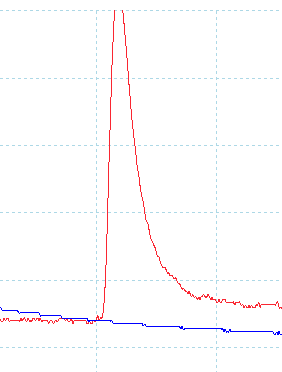
\includegraphics[width=4cm]{diagrams/zjebany.png}
    \caption{Przykład problematycznego pomiaru}
    \label{blad}
\end{wrapfigure} Wyliczone przeze mnie niepewności pomiarów były o dwa rzędy wielkości mniejsze od wartości do których się odnosiły, co silnie sugeruje że uzyskane przeze mnie wyniki można uznać za miarodajne. Jednak uzyskane przeze mnie czasy dryfu, a co za tym idzie wyliczone na ich podstawie prędkości dryfu, dla wysokich wartości napięć dryfu odstawały od reszty wyników. Te odchylenia mogły być spowodowane błędami systematycznymi związanymi ze sposobem określania czasu wykrycia cząstek. Wykorzystana przeze mnie metoda analizy danych pozwalała wyznaczyć tylko przybliżony czas wykrycia cząstki. Dla wysokich wartości napięcia dryfu do wykorzystywanego przez moją metodę zakresu czasów przypada mniejsza ilość pomiarów. Powoduje zmniejszenie jakości dopasowania. Negatywny wpływ na dokładność wyników miała również dyfuzja. Powoduje ona na rozmycie impulsów elektronów, a jej wpływ na wyniki pomiarów był zależny od napięcia dryfu (rozmycie sygnału jest proporcjonalne do czasu dryfu, który z kolei jest odwrotnie proporcjonalny do prędkości dryfu. Sama prędkość dryfu była proporcjonalna do przyłożonego napięcia dryfu). Na niedokładność wyników mogła też wpłynąć konieczność odrzucenia niektórych pomiarów dla wysokich wartości napięć dryfu. W celu uzyskania czasu wykrycia elektronów musiałem być w stanie wyznaczyć maksymalne napięcie na kanale. Jednak dla pomiarów dokonanych dla wysokich napięć dryfu (szczególnie dla pomiarów dokonanych dla detektorów \#2 i \#3) wartości napięcia na kanale B potrafiły wychodzić poza skalę oscyloskopu \ref{blad}. Uniemożliwiało to wyznaczenie maksymalnej wartości napięcia na kanale, w rezultacie zmuszając mnie do odrzucenia takiego pomiaru. Z tego powodu na uśrednione czasy dryfu dla wysokich napięć składają się dane z mniejszej liczby pomiarów, co mogło skutkować zmniejszeniem dokładności otrzymanych danych.

Jako że w czasie przeprowadzania pomiarów ciśnienie i temperatura gazu pozostawały niezmienne, to uzyskane odstępstwa nie mogą być wytłumaczone wachaniami tych wartości

\newpage

\section{Nieudana próba wyznaczenia parametru $\lambda$ związanego z dyfuzją}

Próbowałem przeanalizować dyfuzje deryfujących elektronów w gazie. Na podstawie uzyskanych przeze mnie danych byłem w stanie przybliżyć czas $t_{imp}$ jaki trwał impuls wykrywany przez detektor \#3. Jako że byłem w stanie wyliczyć prędkość z jaką poruszały się elektrony, to uzyskana w ten sposób wartość pozwalała na wyliczenie szerokości sygnału. Z kolei ta szerokość była bezpośrednio związana z parametrem $\lambda$ charakteryzującego dyfuzję

\begin{gather*}
    \sigma = v_{el} t_{imp}\\
    \sigma = \sqrt{2Dt} = \sqrt{2*D*\frac{l}{v_{el}}} = \sqrt{2\frac{1}{3}l\lambda}\\
    v_{el} t_{imp} = \sqrt{2Dt} = \sqrt{2D\frac{l}{v_{el}}} = \sqrt{2\frac{1}{3}l\lambda}\\
    \lambda = \frac{3v^2_{ele}t^2_{imp}}{2l}
\end{gather*}

Gdzie $l$ jest dystansem przebytym przez elektrony

\begin{figure*}[h]
    \centering
    \resizebox{0.9\textwidth}{!}{%% Creator: Matplotlib, PGF backend
%%
%% To include the figure in your LaTeX document, write
%%   \input{<filename>.pgf}
%%
%% Make sure the required packages are loaded in your preamble
%%   \usepackage{pgf}
%%
%% and, on pdftex
%%   \usepackage[utf8]{inputenc}\DeclareUnicodeCharacter{2212}{-}
%%
%% or, on luatex and xetex
%%   \usepackage{unicode-math}
%%
%% Figures using additional raster images can only be included by \input if
%% they are in the same directory as the main LaTeX file. For loading figures
%% from other directories you can use the `import` package
%%   \usepackage{import}
%%
%% and then include the figures with
%%   \import{<path to file>}{<filename>.pgf}
%%
%% Matplotlib used the following preamble
%%   \usepackage{fontspec}
%%   \setmainfont{DejaVuSerif.ttf}[Path=C:/Users/wojte/Envs/yeet/Lib/site-packages/matplotlib/mpl-data/fonts/ttf/]
%%   \setsansfont{DejaVuSans.ttf}[Path=C:/Users/wojte/Envs/yeet/Lib/site-packages/matplotlib/mpl-data/fonts/ttf/]
%%   \setmonofont{DejaVuSansMono.ttf}[Path=C:/Users/wojte/Envs/yeet/Lib/site-packages/matplotlib/mpl-data/fonts/ttf/]
%%
\begingroup%
\makeatletter%
\begin{pgfpicture}%
\pgfpathrectangle{\pgfpointorigin}{\pgfqpoint{9.220000in}{5.160000in}}%
\pgfusepath{use as bounding box, clip}%
\begin{pgfscope}%
\pgfsetbuttcap%
\pgfsetmiterjoin%
\definecolor{currentfill}{rgb}{1.000000,1.000000,1.000000}%
\pgfsetfillcolor{currentfill}%
\pgfsetlinewidth{0.000000pt}%
\definecolor{currentstroke}{rgb}{1.000000,1.000000,1.000000}%
\pgfsetstrokecolor{currentstroke}%
\pgfsetdash{}{0pt}%
\pgfpathmoveto{\pgfqpoint{0.000000in}{0.000000in}}%
\pgfpathlineto{\pgfqpoint{9.220000in}{0.000000in}}%
\pgfpathlineto{\pgfqpoint{9.220000in}{5.160000in}}%
\pgfpathlineto{\pgfqpoint{0.000000in}{5.160000in}}%
\pgfpathclose%
\pgfusepath{fill}%
\end{pgfscope}%
\begin{pgfscope}%
\pgfsetbuttcap%
\pgfsetmiterjoin%
\definecolor{currentfill}{rgb}{1.000000,1.000000,1.000000}%
\pgfsetfillcolor{currentfill}%
\pgfsetlinewidth{0.000000pt}%
\definecolor{currentstroke}{rgb}{0.000000,0.000000,0.000000}%
\pgfsetstrokecolor{currentstroke}%
\pgfsetstrokeopacity{0.000000}%
\pgfsetdash{}{0pt}%
\pgfpathmoveto{\pgfqpoint{1.152500in}{0.903000in}}%
\pgfpathlineto{\pgfqpoint{8.298000in}{0.903000in}}%
\pgfpathlineto{\pgfqpoint{8.298000in}{4.540800in}}%
\pgfpathlineto{\pgfqpoint{1.152500in}{4.540800in}}%
\pgfpathclose%
\pgfusepath{fill}%
\end{pgfscope}%
\begin{pgfscope}%
\pgfsetbuttcap%
\pgfsetroundjoin%
\definecolor{currentfill}{rgb}{0.000000,0.000000,0.000000}%
\pgfsetfillcolor{currentfill}%
\pgfsetlinewidth{0.803000pt}%
\definecolor{currentstroke}{rgb}{0.000000,0.000000,0.000000}%
\pgfsetstrokecolor{currentstroke}%
\pgfsetdash{}{0pt}%
\pgfsys@defobject{currentmarker}{\pgfqpoint{0.000000in}{-0.048611in}}{\pgfqpoint{0.000000in}{0.000000in}}{%
\pgfpathmoveto{\pgfqpoint{0.000000in}{0.000000in}}%
\pgfpathlineto{\pgfqpoint{0.000000in}{-0.048611in}}%
\pgfusepath{stroke,fill}%
}%
\begin{pgfscope}%
\pgfsys@transformshift{1.620747in}{0.903000in}%
\pgfsys@useobject{currentmarker}{}%
\end{pgfscope}%
\end{pgfscope}%
\begin{pgfscope}%
\definecolor{textcolor}{rgb}{0.000000,0.000000,0.000000}%
\pgfsetstrokecolor{textcolor}%
\pgfsetfillcolor{textcolor}%
\pgftext[x=1.620747in,y=0.805778in,,top]{\color{textcolor}\sffamily\fontsize{10.000000}{12.000000}\selectfont 0.50}%
\end{pgfscope}%
\begin{pgfscope}%
\pgfsetbuttcap%
\pgfsetroundjoin%
\definecolor{currentfill}{rgb}{0.000000,0.000000,0.000000}%
\pgfsetfillcolor{currentfill}%
\pgfsetlinewidth{0.803000pt}%
\definecolor{currentstroke}{rgb}{0.000000,0.000000,0.000000}%
\pgfsetstrokecolor{currentstroke}%
\pgfsetdash{}{0pt}%
\pgfsys@defobject{currentmarker}{\pgfqpoint{0.000000in}{-0.048611in}}{\pgfqpoint{0.000000in}{0.000000in}}{%
\pgfpathmoveto{\pgfqpoint{0.000000in}{0.000000in}}%
\pgfpathlineto{\pgfqpoint{0.000000in}{-0.048611in}}%
\pgfusepath{stroke,fill}%
}%
\begin{pgfscope}%
\pgfsys@transformshift{2.504461in}{0.903000in}%
\pgfsys@useobject{currentmarker}{}%
\end{pgfscope}%
\end{pgfscope}%
\begin{pgfscope}%
\definecolor{textcolor}{rgb}{0.000000,0.000000,0.000000}%
\pgfsetstrokecolor{textcolor}%
\pgfsetfillcolor{textcolor}%
\pgftext[x=2.504461in,y=0.805778in,,top]{\color{textcolor}\sffamily\fontsize{10.000000}{12.000000}\selectfont 0.75}%
\end{pgfscope}%
\begin{pgfscope}%
\pgfsetbuttcap%
\pgfsetroundjoin%
\definecolor{currentfill}{rgb}{0.000000,0.000000,0.000000}%
\pgfsetfillcolor{currentfill}%
\pgfsetlinewidth{0.803000pt}%
\definecolor{currentstroke}{rgb}{0.000000,0.000000,0.000000}%
\pgfsetstrokecolor{currentstroke}%
\pgfsetdash{}{0pt}%
\pgfsys@defobject{currentmarker}{\pgfqpoint{0.000000in}{-0.048611in}}{\pgfqpoint{0.000000in}{0.000000in}}{%
\pgfpathmoveto{\pgfqpoint{0.000000in}{0.000000in}}%
\pgfpathlineto{\pgfqpoint{0.000000in}{-0.048611in}}%
\pgfusepath{stroke,fill}%
}%
\begin{pgfscope}%
\pgfsys@transformshift{3.388175in}{0.903000in}%
\pgfsys@useobject{currentmarker}{}%
\end{pgfscope}%
\end{pgfscope}%
\begin{pgfscope}%
\definecolor{textcolor}{rgb}{0.000000,0.000000,0.000000}%
\pgfsetstrokecolor{textcolor}%
\pgfsetfillcolor{textcolor}%
\pgftext[x=3.388175in,y=0.805778in,,top]{\color{textcolor}\sffamily\fontsize{10.000000}{12.000000}\selectfont 1.00}%
\end{pgfscope}%
\begin{pgfscope}%
\pgfsetbuttcap%
\pgfsetroundjoin%
\definecolor{currentfill}{rgb}{0.000000,0.000000,0.000000}%
\pgfsetfillcolor{currentfill}%
\pgfsetlinewidth{0.803000pt}%
\definecolor{currentstroke}{rgb}{0.000000,0.000000,0.000000}%
\pgfsetstrokecolor{currentstroke}%
\pgfsetdash{}{0pt}%
\pgfsys@defobject{currentmarker}{\pgfqpoint{0.000000in}{-0.048611in}}{\pgfqpoint{0.000000in}{0.000000in}}{%
\pgfpathmoveto{\pgfqpoint{0.000000in}{0.000000in}}%
\pgfpathlineto{\pgfqpoint{0.000000in}{-0.048611in}}%
\pgfusepath{stroke,fill}%
}%
\begin{pgfscope}%
\pgfsys@transformshift{4.271890in}{0.903000in}%
\pgfsys@useobject{currentmarker}{}%
\end{pgfscope}%
\end{pgfscope}%
\begin{pgfscope}%
\definecolor{textcolor}{rgb}{0.000000,0.000000,0.000000}%
\pgfsetstrokecolor{textcolor}%
\pgfsetfillcolor{textcolor}%
\pgftext[x=4.271890in,y=0.805778in,,top]{\color{textcolor}\sffamily\fontsize{10.000000}{12.000000}\selectfont 1.25}%
\end{pgfscope}%
\begin{pgfscope}%
\pgfsetbuttcap%
\pgfsetroundjoin%
\definecolor{currentfill}{rgb}{0.000000,0.000000,0.000000}%
\pgfsetfillcolor{currentfill}%
\pgfsetlinewidth{0.803000pt}%
\definecolor{currentstroke}{rgb}{0.000000,0.000000,0.000000}%
\pgfsetstrokecolor{currentstroke}%
\pgfsetdash{}{0pt}%
\pgfsys@defobject{currentmarker}{\pgfqpoint{0.000000in}{-0.048611in}}{\pgfqpoint{0.000000in}{0.000000in}}{%
\pgfpathmoveto{\pgfqpoint{0.000000in}{0.000000in}}%
\pgfpathlineto{\pgfqpoint{0.000000in}{-0.048611in}}%
\pgfusepath{stroke,fill}%
}%
\begin{pgfscope}%
\pgfsys@transformshift{5.155604in}{0.903000in}%
\pgfsys@useobject{currentmarker}{}%
\end{pgfscope}%
\end{pgfscope}%
\begin{pgfscope}%
\definecolor{textcolor}{rgb}{0.000000,0.000000,0.000000}%
\pgfsetstrokecolor{textcolor}%
\pgfsetfillcolor{textcolor}%
\pgftext[x=5.155604in,y=0.805778in,,top]{\color{textcolor}\sffamily\fontsize{10.000000}{12.000000}\selectfont 1.50}%
\end{pgfscope}%
\begin{pgfscope}%
\pgfsetbuttcap%
\pgfsetroundjoin%
\definecolor{currentfill}{rgb}{0.000000,0.000000,0.000000}%
\pgfsetfillcolor{currentfill}%
\pgfsetlinewidth{0.803000pt}%
\definecolor{currentstroke}{rgb}{0.000000,0.000000,0.000000}%
\pgfsetstrokecolor{currentstroke}%
\pgfsetdash{}{0pt}%
\pgfsys@defobject{currentmarker}{\pgfqpoint{0.000000in}{-0.048611in}}{\pgfqpoint{0.000000in}{0.000000in}}{%
\pgfpathmoveto{\pgfqpoint{0.000000in}{0.000000in}}%
\pgfpathlineto{\pgfqpoint{0.000000in}{-0.048611in}}%
\pgfusepath{stroke,fill}%
}%
\begin{pgfscope}%
\pgfsys@transformshift{6.039318in}{0.903000in}%
\pgfsys@useobject{currentmarker}{}%
\end{pgfscope}%
\end{pgfscope}%
\begin{pgfscope}%
\definecolor{textcolor}{rgb}{0.000000,0.000000,0.000000}%
\pgfsetstrokecolor{textcolor}%
\pgfsetfillcolor{textcolor}%
\pgftext[x=6.039318in,y=0.805778in,,top]{\color{textcolor}\sffamily\fontsize{10.000000}{12.000000}\selectfont 1.75}%
\end{pgfscope}%
\begin{pgfscope}%
\pgfsetbuttcap%
\pgfsetroundjoin%
\definecolor{currentfill}{rgb}{0.000000,0.000000,0.000000}%
\pgfsetfillcolor{currentfill}%
\pgfsetlinewidth{0.803000pt}%
\definecolor{currentstroke}{rgb}{0.000000,0.000000,0.000000}%
\pgfsetstrokecolor{currentstroke}%
\pgfsetdash{}{0pt}%
\pgfsys@defobject{currentmarker}{\pgfqpoint{0.000000in}{-0.048611in}}{\pgfqpoint{0.000000in}{0.000000in}}{%
\pgfpathmoveto{\pgfqpoint{0.000000in}{0.000000in}}%
\pgfpathlineto{\pgfqpoint{0.000000in}{-0.048611in}}%
\pgfusepath{stroke,fill}%
}%
\begin{pgfscope}%
\pgfsys@transformshift{6.923033in}{0.903000in}%
\pgfsys@useobject{currentmarker}{}%
\end{pgfscope}%
\end{pgfscope}%
\begin{pgfscope}%
\definecolor{textcolor}{rgb}{0.000000,0.000000,0.000000}%
\pgfsetstrokecolor{textcolor}%
\pgfsetfillcolor{textcolor}%
\pgftext[x=6.923033in,y=0.805778in,,top]{\color{textcolor}\sffamily\fontsize{10.000000}{12.000000}\selectfont 2.00}%
\end{pgfscope}%
\begin{pgfscope}%
\pgfsetbuttcap%
\pgfsetroundjoin%
\definecolor{currentfill}{rgb}{0.000000,0.000000,0.000000}%
\pgfsetfillcolor{currentfill}%
\pgfsetlinewidth{0.803000pt}%
\definecolor{currentstroke}{rgb}{0.000000,0.000000,0.000000}%
\pgfsetstrokecolor{currentstroke}%
\pgfsetdash{}{0pt}%
\pgfsys@defobject{currentmarker}{\pgfqpoint{0.000000in}{-0.048611in}}{\pgfqpoint{0.000000in}{0.000000in}}{%
\pgfpathmoveto{\pgfqpoint{0.000000in}{0.000000in}}%
\pgfpathlineto{\pgfqpoint{0.000000in}{-0.048611in}}%
\pgfusepath{stroke,fill}%
}%
\begin{pgfscope}%
\pgfsys@transformshift{7.806747in}{0.903000in}%
\pgfsys@useobject{currentmarker}{}%
\end{pgfscope}%
\end{pgfscope}%
\begin{pgfscope}%
\definecolor{textcolor}{rgb}{0.000000,0.000000,0.000000}%
\pgfsetstrokecolor{textcolor}%
\pgfsetfillcolor{textcolor}%
\pgftext[x=7.806747in,y=0.805778in,,top]{\color{textcolor}\sffamily\fontsize{10.000000}{12.000000}\selectfont 2.25}%
\end{pgfscope}%
\begin{pgfscope}%
\definecolor{textcolor}{rgb}{0.000000,0.000000,0.000000}%
\pgfsetstrokecolor{textcolor}%
\pgfsetfillcolor{textcolor}%
\pgftext[x=4.725250in,y=0.615809in,,top]{\color{textcolor}\sffamily\fontsize{20.000000}{12.000000}\selectfont $\frac{E}{p} \left[\frac{V}{cm*hPa}\right]$}%
\end{pgfscope}%
\begin{pgfscope}%
\pgfsetbuttcap%
\pgfsetroundjoin%
\definecolor{currentfill}{rgb}{0.000000,0.000000,0.000000}%
\pgfsetfillcolor{currentfill}%
\pgfsetlinewidth{0.803000pt}%
\definecolor{currentstroke}{rgb}{0.000000,0.000000,0.000000}%
\pgfsetstrokecolor{currentstroke}%
\pgfsetdash{}{0pt}%
\pgfsys@defobject{currentmarker}{\pgfqpoint{-0.048611in}{0.000000in}}{\pgfqpoint{-0.000000in}{0.000000in}}{%
\pgfpathmoveto{\pgfqpoint{-0.000000in}{0.000000in}}%
\pgfpathlineto{\pgfqpoint{-0.048611in}{0.000000in}}%
\pgfusepath{stroke,fill}%
}%
\begin{pgfscope}%
\pgfsys@transformshift{1.152500in}{1.442333in}%
\pgfsys@useobject{currentmarker}{}%
\end{pgfscope}%
\end{pgfscope}%
\begin{pgfscope}%
\definecolor{textcolor}{rgb}{0.000000,0.000000,0.000000}%
\pgfsetstrokecolor{textcolor}%
\pgfsetfillcolor{textcolor}%
\pgftext[x=0.657668in, y=1.389571in, left, base]{\color{textcolor}\sffamily\fontsize{10.000000}{12.000000}\selectfont 0.015}%
\end{pgfscope}%
\begin{pgfscope}%
\pgfsetbuttcap%
\pgfsetroundjoin%
\definecolor{currentfill}{rgb}{0.000000,0.000000,0.000000}%
\pgfsetfillcolor{currentfill}%
\pgfsetlinewidth{0.803000pt}%
\definecolor{currentstroke}{rgb}{0.000000,0.000000,0.000000}%
\pgfsetstrokecolor{currentstroke}%
\pgfsetdash{}{0pt}%
\pgfsys@defobject{currentmarker}{\pgfqpoint{-0.048611in}{0.000000in}}{\pgfqpoint{-0.000000in}{0.000000in}}{%
\pgfpathmoveto{\pgfqpoint{-0.000000in}{0.000000in}}%
\pgfpathlineto{\pgfqpoint{-0.048611in}{0.000000in}}%
\pgfusepath{stroke,fill}%
}%
\begin{pgfscope}%
\pgfsys@transformshift{1.152500in}{2.130445in}%
\pgfsys@useobject{currentmarker}{}%
\end{pgfscope}%
\end{pgfscope}%
\begin{pgfscope}%
\definecolor{textcolor}{rgb}{0.000000,0.000000,0.000000}%
\pgfsetstrokecolor{textcolor}%
\pgfsetfillcolor{textcolor}%
\pgftext[x=0.657668in, y=2.077683in, left, base]{\color{textcolor}\sffamily\fontsize{10.000000}{12.000000}\selectfont 0.020}%
\end{pgfscope}%
\begin{pgfscope}%
\pgfsetbuttcap%
\pgfsetroundjoin%
\definecolor{currentfill}{rgb}{0.000000,0.000000,0.000000}%
\pgfsetfillcolor{currentfill}%
\pgfsetlinewidth{0.803000pt}%
\definecolor{currentstroke}{rgb}{0.000000,0.000000,0.000000}%
\pgfsetstrokecolor{currentstroke}%
\pgfsetdash{}{0pt}%
\pgfsys@defobject{currentmarker}{\pgfqpoint{-0.048611in}{0.000000in}}{\pgfqpoint{-0.000000in}{0.000000in}}{%
\pgfpathmoveto{\pgfqpoint{-0.000000in}{0.000000in}}%
\pgfpathlineto{\pgfqpoint{-0.048611in}{0.000000in}}%
\pgfusepath{stroke,fill}%
}%
\begin{pgfscope}%
\pgfsys@transformshift{1.152500in}{2.818557in}%
\pgfsys@useobject{currentmarker}{}%
\end{pgfscope}%
\end{pgfscope}%
\begin{pgfscope}%
\definecolor{textcolor}{rgb}{0.000000,0.000000,0.000000}%
\pgfsetstrokecolor{textcolor}%
\pgfsetfillcolor{textcolor}%
\pgftext[x=0.657668in, y=2.765796in, left, base]{\color{textcolor}\sffamily\fontsize{10.000000}{12.000000}\selectfont 0.025}%
\end{pgfscope}%
\begin{pgfscope}%
\pgfsetbuttcap%
\pgfsetroundjoin%
\definecolor{currentfill}{rgb}{0.000000,0.000000,0.000000}%
\pgfsetfillcolor{currentfill}%
\pgfsetlinewidth{0.803000pt}%
\definecolor{currentstroke}{rgb}{0.000000,0.000000,0.000000}%
\pgfsetstrokecolor{currentstroke}%
\pgfsetdash{}{0pt}%
\pgfsys@defobject{currentmarker}{\pgfqpoint{-0.048611in}{0.000000in}}{\pgfqpoint{-0.000000in}{0.000000in}}{%
\pgfpathmoveto{\pgfqpoint{-0.000000in}{0.000000in}}%
\pgfpathlineto{\pgfqpoint{-0.048611in}{0.000000in}}%
\pgfusepath{stroke,fill}%
}%
\begin{pgfscope}%
\pgfsys@transformshift{1.152500in}{3.506669in}%
\pgfsys@useobject{currentmarker}{}%
\end{pgfscope}%
\end{pgfscope}%
\begin{pgfscope}%
\definecolor{textcolor}{rgb}{0.000000,0.000000,0.000000}%
\pgfsetstrokecolor{textcolor}%
\pgfsetfillcolor{textcolor}%
\pgftext[x=0.657668in, y=3.453908in, left, base]{\color{textcolor}\sffamily\fontsize{10.000000}{12.000000}\selectfont 0.030}%
\end{pgfscope}%
\begin{pgfscope}%
\pgfsetbuttcap%
\pgfsetroundjoin%
\definecolor{currentfill}{rgb}{0.000000,0.000000,0.000000}%
\pgfsetfillcolor{currentfill}%
\pgfsetlinewidth{0.803000pt}%
\definecolor{currentstroke}{rgb}{0.000000,0.000000,0.000000}%
\pgfsetstrokecolor{currentstroke}%
\pgfsetdash{}{0pt}%
\pgfsys@defobject{currentmarker}{\pgfqpoint{-0.048611in}{0.000000in}}{\pgfqpoint{-0.000000in}{0.000000in}}{%
\pgfpathmoveto{\pgfqpoint{-0.000000in}{0.000000in}}%
\pgfpathlineto{\pgfqpoint{-0.048611in}{0.000000in}}%
\pgfusepath{stroke,fill}%
}%
\begin{pgfscope}%
\pgfsys@transformshift{1.152500in}{4.194781in}%
\pgfsys@useobject{currentmarker}{}%
\end{pgfscope}%
\end{pgfscope}%
\begin{pgfscope}%
\definecolor{textcolor}{rgb}{0.000000,0.000000,0.000000}%
\pgfsetstrokecolor{textcolor}%
\pgfsetfillcolor{textcolor}%
\pgftext[x=0.657668in, y=4.142020in, left, base]{\color{textcolor}\sffamily\fontsize{10.000000}{12.000000}\selectfont 0.035}%
\end{pgfscope}%
\begin{pgfscope}%
\definecolor{textcolor}{rgb}{0.000000,0.000000,0.000000}%
\pgfsetstrokecolor{textcolor}%
\pgfsetfillcolor{textcolor}%
\pgftext[x=0.602112in,y=2.721900in,,bottom,rotate=90.000000]{\color{textcolor}\sffamily\fontsize{20.000000}{12.000000}\selectfont $\lambda$}%
\end{pgfscope}%
\begin{pgfscope}%
\pgfpathrectangle{\pgfqpoint{1.152500in}{0.903000in}}{\pgfqpoint{7.145500in}{3.637800in}}%
\pgfusepath{clip}%
\pgfsetrectcap%
\pgfsetroundjoin%
\pgfsetlinewidth{1.505625pt}%
\definecolor{currentstroke}{rgb}{0.121569,0.466667,0.705882}%
\pgfsetstrokecolor{currentstroke}%
\pgfsetdash{}{0pt}%
\pgfpathmoveto{\pgfqpoint{1.477295in}{1.301444in}}%
\pgfpathlineto{\pgfqpoint{1.747958in}{1.624107in}}%
\pgfpathlineto{\pgfqpoint{2.018621in}{1.236806in}}%
\pgfpathlineto{\pgfqpoint{2.289284in}{1.346775in}}%
\pgfpathlineto{\pgfqpoint{2.559947in}{1.254662in}}%
\pgfpathlineto{\pgfqpoint{2.830610in}{1.068355in}}%
\pgfpathlineto{\pgfqpoint{3.101273in}{1.087323in}}%
\pgfpathlineto{\pgfqpoint{3.371936in}{1.112577in}}%
\pgfpathlineto{\pgfqpoint{3.642598in}{1.220973in}}%
\pgfpathlineto{\pgfqpoint{3.913261in}{1.219206in}}%
\pgfpathlineto{\pgfqpoint{4.183924in}{1.350340in}}%
\pgfpathlineto{\pgfqpoint{4.454587in}{1.372096in}}%
\pgfpathlineto{\pgfqpoint{4.725250in}{1.399637in}}%
\pgfpathlineto{\pgfqpoint{4.995913in}{1.461122in}}%
\pgfpathlineto{\pgfqpoint{5.266576in}{1.462281in}}%
\pgfpathlineto{\pgfqpoint{5.537239in}{1.523445in}}%
\pgfpathlineto{\pgfqpoint{5.807902in}{1.615126in}}%
\pgfpathlineto{\pgfqpoint{6.078564in}{1.655855in}}%
\pgfpathlineto{\pgfqpoint{6.349227in}{1.720046in}}%
\pgfpathlineto{\pgfqpoint{6.619890in}{1.704309in}}%
\pgfpathlineto{\pgfqpoint{6.890553in}{1.879754in}}%
\pgfpathlineto{\pgfqpoint{7.161216in}{1.955718in}}%
\pgfpathlineto{\pgfqpoint{7.431879in}{2.203026in}}%
\pgfpathlineto{\pgfqpoint{7.702542in}{2.245441in}}%
\pgfpathlineto{\pgfqpoint{7.973205in}{2.294250in}}%
\pgfusepath{stroke}%
\end{pgfscope}%
\begin{pgfscope}%
\pgfpathrectangle{\pgfqpoint{1.152500in}{0.903000in}}{\pgfqpoint{7.145500in}{3.637800in}}%
\pgfusepath{clip}%
\pgfsetrectcap%
\pgfsetroundjoin%
\pgfsetlinewidth{1.505625pt}%
\definecolor{currentstroke}{rgb}{1.000000,0.498039,0.054902}%
\pgfsetstrokecolor{currentstroke}%
\pgfsetdash{}{0pt}%
\pgfpathmoveto{\pgfqpoint{1.477295in}{1.597264in}}%
\pgfpathlineto{\pgfqpoint{1.747958in}{1.372487in}}%
\pgfpathlineto{\pgfqpoint{2.018621in}{1.323927in}}%
\pgfpathlineto{\pgfqpoint{2.289284in}{1.265302in}}%
\pgfpathlineto{\pgfqpoint{2.559947in}{1.283132in}}%
\pgfpathlineto{\pgfqpoint{2.830610in}{1.307474in}}%
\pgfpathlineto{\pgfqpoint{3.101273in}{1.449374in}}%
\pgfpathlineto{\pgfqpoint{3.371936in}{1.379990in}}%
\pgfpathlineto{\pgfqpoint{3.642598in}{1.247039in}}%
\pgfpathlineto{\pgfqpoint{3.913261in}{1.621948in}}%
\pgfpathlineto{\pgfqpoint{4.183924in}{1.777949in}}%
\pgfpathlineto{\pgfqpoint{4.454587in}{1.866075in}}%
\pgfpathlineto{\pgfqpoint{4.725250in}{2.097106in}}%
\pgfpathlineto{\pgfqpoint{4.995913in}{1.974156in}}%
\pgfpathlineto{\pgfqpoint{5.266576in}{2.113254in}}%
\pgfpathlineto{\pgfqpoint{5.537239in}{2.250468in}}%
\pgfpathlineto{\pgfqpoint{5.807902in}{2.419794in}}%
\pgfpathlineto{\pgfqpoint{6.078564in}{2.567271in}}%
\pgfpathlineto{\pgfqpoint{6.349227in}{2.869479in}}%
\pgfpathlineto{\pgfqpoint{6.619890in}{3.008964in}}%
\pgfpathlineto{\pgfqpoint{6.890553in}{3.259836in}}%
\pgfpathlineto{\pgfqpoint{7.161216in}{3.524747in}}%
\pgfpathlineto{\pgfqpoint{7.431879in}{3.975295in}}%
\pgfpathlineto{\pgfqpoint{7.702542in}{4.181659in}}%
\pgfpathlineto{\pgfqpoint{7.973205in}{4.375445in}}%
\pgfusepath{stroke}%
\end{pgfscope}%
\begin{pgfscope}%
\pgfsetrectcap%
\pgfsetmiterjoin%
\pgfsetlinewidth{0.803000pt}%
\definecolor{currentstroke}{rgb}{0.000000,0.000000,0.000000}%
\pgfsetstrokecolor{currentstroke}%
\pgfsetdash{}{0pt}%
\pgfpathmoveto{\pgfqpoint{1.152500in}{0.903000in}}%
\pgfpathlineto{\pgfqpoint{1.152500in}{4.540800in}}%
\pgfusepath{stroke}%
\end{pgfscope}%
\begin{pgfscope}%
\pgfsetrectcap%
\pgfsetmiterjoin%
\pgfsetlinewidth{0.803000pt}%
\definecolor{currentstroke}{rgb}{0.000000,0.000000,0.000000}%
\pgfsetstrokecolor{currentstroke}%
\pgfsetdash{}{0pt}%
\pgfpathmoveto{\pgfqpoint{8.298000in}{0.903000in}}%
\pgfpathlineto{\pgfqpoint{8.298000in}{4.540800in}}%
\pgfusepath{stroke}%
\end{pgfscope}%
\begin{pgfscope}%
\pgfsetrectcap%
\pgfsetmiterjoin%
\pgfsetlinewidth{0.803000pt}%
\definecolor{currentstroke}{rgb}{0.000000,0.000000,0.000000}%
\pgfsetstrokecolor{currentstroke}%
\pgfsetdash{}{0pt}%
\pgfpathmoveto{\pgfqpoint{1.152500in}{0.903000in}}%
\pgfpathlineto{\pgfqpoint{8.298000in}{0.903000in}}%
\pgfusepath{stroke}%
\end{pgfscope}%
\begin{pgfscope}%
\pgfsetrectcap%
\pgfsetmiterjoin%
\pgfsetlinewidth{0.803000pt}%
\definecolor{currentstroke}{rgb}{0.000000,0.000000,0.000000}%
\pgfsetstrokecolor{currentstroke}%
\pgfsetdash{}{0pt}%
\pgfpathmoveto{\pgfqpoint{1.152500in}{4.540800in}}%
\pgfpathlineto{\pgfqpoint{8.298000in}{4.540800in}}%
\pgfusepath{stroke}%
\end{pgfscope}%
\begin{pgfscope}%
\definecolor{textcolor}{rgb}{0.000000,0.000000,0.000000}%
\pgfsetstrokecolor{textcolor}%
\pgfsetfillcolor{textcolor}%
\pgftext[x=4.725250in,y=4.624133in,,base]{\color{textcolor}\sffamily\fontsize{20.000000}{14.400000}\selectfont wyliczone wartośći $\lambda$ w zależności od $\frac{E}{p}$}%
\end{pgfscope}%
\end{pgfpicture}%
\makeatother%
\endgroup%
}
    \caption{Pomarańczowa łamana reprezentuje wartości $\lambda$ uzyskane dla pomiarów między detektorami \#2 i \#3, a niebieska między detektorami \#1 a \#3}
\end{figure*}

\begin{table}[h]
    \centering
    \caption{Uśrednione wartości}
    \label{tab:my-table}
    \begin{tabular}{|l|l|}
    \hline
    lambda   13            & 0.016 \\ \hline
    odchylenie standardowe & 0.003 \\ \hline
    lambda 23              & 0.021 \\ \hline
    odchylenie standardowe & 0.007 \\ \hline
    \end{tabular}
    \end{table}

Okazało się jednak ze uzyskane przeze mnie wyniki nie zgadzały się z przewidywaniami. Analizując dane uzyskane dla pomiarów wykonanych dla detektorów \#2 i \#3 uzyskiwałem znacząco inne wyniki niż dla pomiarów wykonanych dla detektorów \#1 i \#3. Wyliczona wartość parametru $\lambda$ nie była również stała dla pomiarów wykonanych dla tych samych detektorów, ale dla różnych wartości napięcia dryfu. Wyliczone przeze mnie wartości $\lambda$ powinny być niezależne od tych parametrów. Na niepoprawność wyników znaczący wpływ mógł mieć błąd systematyczny związany z wykorzystaną przeze mnie metodą analizy danych.

\section{Podsumowanie}

Wyznaczona przeze mnie wartość $\mu$ wyniosła $0.703 \pm 0.006$. Otrzymany przeze mnie wynik okazał się być zgodny z przewidywaniami teoretycznymi oraz wynikami przedstawionymi w opracowaniu dostępnym na stronie pracowni \cite{opracowanie}. W czasie wykonywania pomiarów wykorzystywany przeze mnie układ badawczy zachowywał się zgodnie z przewidywaniami. Wyliczone przeze mnie błędy pomiarowe okazały się być na tyle małe, że korelujące z nimi dane uznałem za miarodajne. Pomimo pewnych odchyleń występujących dla wyższych napięć dryfu dopasowane przeze mnie funkcje okazały się być dobrą reprezentacją otrzymanych przeze mnie wyników. Próba wyznaczenia parametru $\lambda$ charakteryzującego dyfuzję zakończyła się niepowodzeniem najprawdopodobniej spowodowanym błędem systematycznym wykorzystywanej przeze mnie metody analizy danych

\bibliographystyle{unsrt}
\bibliography{References}


\end{document}


